% Generated by Sphinx.
\def\sphinxdocclass{report}
\documentclass[letterpaper,10pt,openany,oneside]{sphinxmanual}
\usepackage[utf8]{inputenc}
\DeclareUnicodeCharacter{00A0}{\nobreakspace}
\usepackage[T1]{fontenc}
\usepackage[english]{babel}
\usepackage{times}
\usepackage[Bjarne]{fncychap}
\usepackage{longtable}
\usepackage{sphinx}
\usepackage{multirow}


\title{Pandemic with MPI}
\date{March 29, 2016}
\release{}
\author{CSInParallel Project}
\newcommand{\sphinxlogo}{}
\renewcommand{\releasename}{}
\makeindex

\makeatletter
\def\PYG@reset{\let\PYG@it=\relax \let\PYG@bf=\relax%
    \let\PYG@ul=\relax \let\PYG@tc=\relax%
    \let\PYG@bc=\relax \let\PYG@ff=\relax}
\def\PYG@tok#1{\csname PYG@tok@#1\endcsname}
\def\PYG@toks#1+{\ifx\relax#1\empty\else%
    \PYG@tok{#1}\expandafter\PYG@toks\fi}
\def\PYG@do#1{\PYG@bc{\PYG@tc{\PYG@ul{%
    \PYG@it{\PYG@bf{\PYG@ff{#1}}}}}}}
\def\PYG#1#2{\PYG@reset\PYG@toks#1+\relax+\PYG@do{#2}}

\expandafter\def\csname PYG@tok@gd\endcsname{\def\PYG@tc##1{\textcolor[rgb]{0.63,0.00,0.00}{##1}}}
\expandafter\def\csname PYG@tok@gu\endcsname{\let\PYG@bf=\textbf\def\PYG@tc##1{\textcolor[rgb]{0.50,0.00,0.50}{##1}}}
\expandafter\def\csname PYG@tok@gt\endcsname{\def\PYG@tc##1{\textcolor[rgb]{0.00,0.25,0.82}{##1}}}
\expandafter\def\csname PYG@tok@gs\endcsname{\let\PYG@bf=\textbf}
\expandafter\def\csname PYG@tok@gr\endcsname{\def\PYG@tc##1{\textcolor[rgb]{1.00,0.00,0.00}{##1}}}
\expandafter\def\csname PYG@tok@cm\endcsname{\let\PYG@it=\textit\def\PYG@tc##1{\textcolor[rgb]{0.25,0.50,0.56}{##1}}}
\expandafter\def\csname PYG@tok@vg\endcsname{\def\PYG@tc##1{\textcolor[rgb]{0.73,0.38,0.84}{##1}}}
\expandafter\def\csname PYG@tok@m\endcsname{\def\PYG@tc##1{\textcolor[rgb]{0.13,0.50,0.31}{##1}}}
\expandafter\def\csname PYG@tok@mh\endcsname{\def\PYG@tc##1{\textcolor[rgb]{0.13,0.50,0.31}{##1}}}
\expandafter\def\csname PYG@tok@cs\endcsname{\def\PYG@tc##1{\textcolor[rgb]{0.25,0.50,0.56}{##1}}\def\PYG@bc##1{\setlength{\fboxsep}{0pt}\colorbox[rgb]{1.00,0.94,0.94}{\strut ##1}}}
\expandafter\def\csname PYG@tok@ge\endcsname{\let\PYG@it=\textit}
\expandafter\def\csname PYG@tok@vc\endcsname{\def\PYG@tc##1{\textcolor[rgb]{0.73,0.38,0.84}{##1}}}
\expandafter\def\csname PYG@tok@il\endcsname{\def\PYG@tc##1{\textcolor[rgb]{0.13,0.50,0.31}{##1}}}
\expandafter\def\csname PYG@tok@go\endcsname{\def\PYG@tc##1{\textcolor[rgb]{0.19,0.19,0.19}{##1}}}
\expandafter\def\csname PYG@tok@cp\endcsname{\def\PYG@tc##1{\textcolor[rgb]{0.00,0.44,0.13}{##1}}}
\expandafter\def\csname PYG@tok@gi\endcsname{\def\PYG@tc##1{\textcolor[rgb]{0.00,0.63,0.00}{##1}}}
\expandafter\def\csname PYG@tok@gh\endcsname{\let\PYG@bf=\textbf\def\PYG@tc##1{\textcolor[rgb]{0.00,0.00,0.50}{##1}}}
\expandafter\def\csname PYG@tok@ni\endcsname{\let\PYG@bf=\textbf\def\PYG@tc##1{\textcolor[rgb]{0.84,0.33,0.22}{##1}}}
\expandafter\def\csname PYG@tok@nl\endcsname{\let\PYG@bf=\textbf\def\PYG@tc##1{\textcolor[rgb]{0.00,0.13,0.44}{##1}}}
\expandafter\def\csname PYG@tok@nn\endcsname{\let\PYG@bf=\textbf\def\PYG@tc##1{\textcolor[rgb]{0.05,0.52,0.71}{##1}}}
\expandafter\def\csname PYG@tok@no\endcsname{\def\PYG@tc##1{\textcolor[rgb]{0.38,0.68,0.84}{##1}}}
\expandafter\def\csname PYG@tok@na\endcsname{\def\PYG@tc##1{\textcolor[rgb]{0.25,0.44,0.63}{##1}}}
\expandafter\def\csname PYG@tok@nb\endcsname{\def\PYG@tc##1{\textcolor[rgb]{0.00,0.44,0.13}{##1}}}
\expandafter\def\csname PYG@tok@nc\endcsname{\let\PYG@bf=\textbf\def\PYG@tc##1{\textcolor[rgb]{0.05,0.52,0.71}{##1}}}
\expandafter\def\csname PYG@tok@nd\endcsname{\let\PYG@bf=\textbf\def\PYG@tc##1{\textcolor[rgb]{0.33,0.33,0.33}{##1}}}
\expandafter\def\csname PYG@tok@ne\endcsname{\def\PYG@tc##1{\textcolor[rgb]{0.00,0.44,0.13}{##1}}}
\expandafter\def\csname PYG@tok@nf\endcsname{\def\PYG@tc##1{\textcolor[rgb]{0.02,0.16,0.49}{##1}}}
\expandafter\def\csname PYG@tok@si\endcsname{\let\PYG@it=\textit\def\PYG@tc##1{\textcolor[rgb]{0.44,0.63,0.82}{##1}}}
\expandafter\def\csname PYG@tok@s2\endcsname{\def\PYG@tc##1{\textcolor[rgb]{0.25,0.44,0.63}{##1}}}
\expandafter\def\csname PYG@tok@vi\endcsname{\def\PYG@tc##1{\textcolor[rgb]{0.73,0.38,0.84}{##1}}}
\expandafter\def\csname PYG@tok@nt\endcsname{\let\PYG@bf=\textbf\def\PYG@tc##1{\textcolor[rgb]{0.02,0.16,0.45}{##1}}}
\expandafter\def\csname PYG@tok@nv\endcsname{\def\PYG@tc##1{\textcolor[rgb]{0.73,0.38,0.84}{##1}}}
\expandafter\def\csname PYG@tok@s1\endcsname{\def\PYG@tc##1{\textcolor[rgb]{0.25,0.44,0.63}{##1}}}
\expandafter\def\csname PYG@tok@gp\endcsname{\let\PYG@bf=\textbf\def\PYG@tc##1{\textcolor[rgb]{0.78,0.36,0.04}{##1}}}
\expandafter\def\csname PYG@tok@sh\endcsname{\def\PYG@tc##1{\textcolor[rgb]{0.25,0.44,0.63}{##1}}}
\expandafter\def\csname PYG@tok@ow\endcsname{\let\PYG@bf=\textbf\def\PYG@tc##1{\textcolor[rgb]{0.00,0.44,0.13}{##1}}}
\expandafter\def\csname PYG@tok@sx\endcsname{\def\PYG@tc##1{\textcolor[rgb]{0.78,0.36,0.04}{##1}}}
\expandafter\def\csname PYG@tok@bp\endcsname{\def\PYG@tc##1{\textcolor[rgb]{0.00,0.44,0.13}{##1}}}
\expandafter\def\csname PYG@tok@c1\endcsname{\let\PYG@it=\textit\def\PYG@tc##1{\textcolor[rgb]{0.25,0.50,0.56}{##1}}}
\expandafter\def\csname PYG@tok@kc\endcsname{\let\PYG@bf=\textbf\def\PYG@tc##1{\textcolor[rgb]{0.00,0.44,0.13}{##1}}}
\expandafter\def\csname PYG@tok@c\endcsname{\let\PYG@it=\textit\def\PYG@tc##1{\textcolor[rgb]{0.25,0.50,0.56}{##1}}}
\expandafter\def\csname PYG@tok@mf\endcsname{\def\PYG@tc##1{\textcolor[rgb]{0.13,0.50,0.31}{##1}}}
\expandafter\def\csname PYG@tok@err\endcsname{\def\PYG@bc##1{\setlength{\fboxsep}{0pt}\fcolorbox[rgb]{1.00,0.00,0.00}{1,1,1}{\strut ##1}}}
\expandafter\def\csname PYG@tok@kd\endcsname{\let\PYG@bf=\textbf\def\PYG@tc##1{\textcolor[rgb]{0.00,0.44,0.13}{##1}}}
\expandafter\def\csname PYG@tok@ss\endcsname{\def\PYG@tc##1{\textcolor[rgb]{0.32,0.47,0.09}{##1}}}
\expandafter\def\csname PYG@tok@sr\endcsname{\def\PYG@tc##1{\textcolor[rgb]{0.14,0.33,0.53}{##1}}}
\expandafter\def\csname PYG@tok@mo\endcsname{\def\PYG@tc##1{\textcolor[rgb]{0.13,0.50,0.31}{##1}}}
\expandafter\def\csname PYG@tok@mi\endcsname{\def\PYG@tc##1{\textcolor[rgb]{0.13,0.50,0.31}{##1}}}
\expandafter\def\csname PYG@tok@kn\endcsname{\let\PYG@bf=\textbf\def\PYG@tc##1{\textcolor[rgb]{0.00,0.44,0.13}{##1}}}
\expandafter\def\csname PYG@tok@o\endcsname{\def\PYG@tc##1{\textcolor[rgb]{0.40,0.40,0.40}{##1}}}
\expandafter\def\csname PYG@tok@kr\endcsname{\let\PYG@bf=\textbf\def\PYG@tc##1{\textcolor[rgb]{0.00,0.44,0.13}{##1}}}
\expandafter\def\csname PYG@tok@s\endcsname{\def\PYG@tc##1{\textcolor[rgb]{0.25,0.44,0.63}{##1}}}
\expandafter\def\csname PYG@tok@kp\endcsname{\def\PYG@tc##1{\textcolor[rgb]{0.00,0.44,0.13}{##1}}}
\expandafter\def\csname PYG@tok@w\endcsname{\def\PYG@tc##1{\textcolor[rgb]{0.73,0.73,0.73}{##1}}}
\expandafter\def\csname PYG@tok@kt\endcsname{\def\PYG@tc##1{\textcolor[rgb]{0.56,0.13,0.00}{##1}}}
\expandafter\def\csname PYG@tok@sc\endcsname{\def\PYG@tc##1{\textcolor[rgb]{0.25,0.44,0.63}{##1}}}
\expandafter\def\csname PYG@tok@sb\endcsname{\def\PYG@tc##1{\textcolor[rgb]{0.25,0.44,0.63}{##1}}}
\expandafter\def\csname PYG@tok@k\endcsname{\let\PYG@bf=\textbf\def\PYG@tc##1{\textcolor[rgb]{0.00,0.44,0.13}{##1}}}
\expandafter\def\csname PYG@tok@se\endcsname{\let\PYG@bf=\textbf\def\PYG@tc##1{\textcolor[rgb]{0.25,0.44,0.63}{##1}}}
\expandafter\def\csname PYG@tok@sd\endcsname{\let\PYG@it=\textit\def\PYG@tc##1{\textcolor[rgb]{0.25,0.44,0.63}{##1}}}

\def\PYGZbs{\char`\\}
\def\PYGZus{\char`\_}
\def\PYGZob{\char`\{}
\def\PYGZcb{\char`\}}
\def\PYGZca{\char`\^}
\def\PYGZam{\char`\&}
\def\PYGZlt{\char`\<}
\def\PYGZgt{\char`\>}
\def\PYGZsh{\char`\#}
\def\PYGZpc{\char`\%}
\def\PYGZdl{\char`\$}
\def\PYGZti{\char`\~}
% for compatibility with earlier versions
\def\PYGZat{@}
\def\PYGZlb{[}
\def\PYGZrb{]}
\makeatother

\begin{document}

\maketitle
\tableofcontents
\phantomsection\label{index::doc}


In this module you will read about how we can model the spread of infectious diseases computationally.
We can make use of distributed computing with message passing to shorten the time needed to model very large populations,
which can be computationally intensive on a single computer.
Each section linked below explains both the computational model and the code, which uses the
Message Passing Interface Library, or MPI, to build a distributed processing solution.


\chapter{Infectious Disease}
\label{0-Introduction/introduction:pandemic-with-mpi}\label{0-Introduction/introduction:infectious-disease}\label{0-Introduction/introduction::doc}
\textbf{By Aaron Weeden, Shodor Education Foundation, Inc.} \footnote{
For original documentation and code developed by Aaron Weeden, please go to original \href{http://www.shodor.org/petascale/materials/UPModules/infectiousDisease/}{pandemic}.
}

\textbf{Heavily modified by Yu Zhao, Macalester College}

\textbf{Overview}

Epidemiology is the study of infectious disease. Infectious diseases are
said to be “contagious” among people if they are transmittable from one
person to another. Epidemiologists can use models to assist them in
predicting the behavior of infectious diseases. This module will develop
a simple agent-based infectious disease model, develop a parallel
algorithm based on the model, provide a coded implementation for the
algorithm, and explore the scaling of the coded implementation on high
performance cluster resources.

\textbf{Pre-assessment Rubric}

This rubric is to gauge students’ initial knowledge and experience with
the materials presented in this module. Students can be asked to rate their
knowledge and experience on the following scale and in the following
subject areas, bith before and after they complete this module.
\begin{quote}

\textbf{Scale}
\begin{enumerate}
\item {} 
no knowledge, no experience

\item {} 
very little knowledge, very little experience

\item {} 
some knowledge, some experience

\item {} 
a good amount of knowledge, a good amount of experience

\item {} 
high level of knowledge, high level of experience

\end{enumerate}

\textbf{Subject areas}
\begin{itemize}
\item {} 
Disease modeling

\item {} 
Parallel Algorithm Design

\item {} 
Parallel Hardware

\item {} 
MPI programming

\item {} 
OpenMP programming

\item {} 
Using a cluster

\item {} 
Scaling parallel code

\end{itemize}
\end{quote}

The goal of the reading and exercises in this module are to see gains in the above subject areas
after completing it.

\textbf{Model}

The model makes certain assumptions about the spread of the disease. In
particular, it assumes that the disease spreads from one person to
another person with some “contagiousness factor”, that is, some percent
chance that the disease will be transmitted. The model further assumes
that diseases can only be spread from a person who is carrying the
disease, a so-called “infected” person, to a person who is capable of
becoming infected, also known as a “susceptible” person. The disease is
assumed to have a certain incubation period, or “duration” – a length of
time during which the disease remains in the person. The disease is also
assumed to be transmittable only within a certain distance, or
“infection radius”, from a person capable of transmitting the disease.
The model further assumes that each person moves randomly at most 1 unit
in a given direction each day. Finally, the model assumes that after the
duration of the disease within a person, the person can become either
“immune” to the disease, incapable of being further infected or of
infecting other people but still able to move around, or “dead”,
incapable of being further infected, infecting other people, or moving.

The description below explains the various entities in the model. Things
in underlines are entities, things in \textbf{bold} are attributes of the
entities, and things in \emph{italics} refer to entities found elsewhere in
the description.


\includegraphics{img-0.png} (pl. people)
\begin{itemize}
\item {} 
Has a certain \textbf{X location} and a certain \textbf{Y location}, which tell where it is in the \emph{environment}.

\item {} 
Has a certain \textbf{state}, which can be either ‘susceptible’, ‘infected’, ‘immune’, or ‘dead’. States are stored in the memories of \emph{processes} and \emph{threads}. They can also be represented by color (black for susceptible, red for infected, green for immune, no color for dead), or by a ASCII character (o for susceptible, X for infected, I for immune, no character for dead).

\end{itemize}


\includegraphics{img-1.png} \emph{Disease}
\begin{itemize}
\item {} 
Has a certain \textbf{duration}, which is the number of days in which a \emph{person} remains infected.

\item {} 
Has a certain \textbf{contagiousness factor}, which is the likelihood of it spreading from one \emph{person} to another.

\item {} 
Has a certain \textbf{deadliness factor}, which is the likelihood that a \emph{person} will die from the disease. 100 minus this is the likelihood that a \emph{person} will become immune to the disease.

\end{itemize}

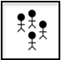
\includegraphics{img-2.png} Environment
\begin{itemize}
\item {} 
Has a certain \textbf{width} and \textbf{height}, which bound the area in which \emph{people} are able to move.

\end{itemize}


\includegraphics{img-3.png} Timer
\begin{itemize}
\item {} 
Counts the \textbf{number of days} that have elapsed in the simulation.

\end{itemize}


\includegraphics{img-4.png} Thread (pl. threads)
\begin{itemize}
\item {} 
A computational entity that controls people and performs computations.

\item {} 
Shares \textbf{memory} with other threads, a space into which threads can read and write data.

\end{itemize}


\includegraphics{img-5.png} Process (pl. processes)
\begin{itemize}
\item {} 
A computational entity that controls people and performs computations.

\item {} 
Has its own private \textbf{memory}, which is a space into which it can read and write data.

\item {} 
Has a certain \textbf{rank}, which identifies it.

\item {} 
Communicates with other processes by \textbf{passing messages}, in which it sends certain data.

\item {} 
Can spawn threads to do work for it.

\item {} 
Keeps count of how many susceptible, infected, immune, and \emph{dead} people exist.

\end{itemize}

\textbf{Introduction to Parallelism}

In parallel processing, rather than having a single program execute
tasks in a sequence, the program is split among multiple “execution
flows” executing tasks in parallel, i.e. at the same time. The term
“execution flow” refers to a discrete computational entity that performs
processes autonomously. A common synonym is “execution context”; “flow”
is chosen here because it evokes the stream of instructions that each
entity processes.

Execution flows have more specific names depending on the flavor of
parallelism being utilized. In “distributed memory” parallelism, in
which execution flows keep their own private memories (separate from the
memories of other execution flows), execution flows are known as
“processes”. In order for one process to access the memory of another
process, the data must be communicated, commonly by a technique known as
“message passing”. The standard of message passing considered in this
module is defined by the “Message Passing Interface (MPI)”, which
defines a set of primitives for packaging up data and sending them
between processes.

In another flavor of parallelism known as “shared memory”, in which
execution flows share a memory space among them, the execution flows are
known as “threads”. Threads are able to read and write to and from
memory without having to send messages. \footnote{
It should be noted that shared memory is really just a form of fast message passing. Threads must communicate, just as processes must, but threads get to communicate at bus speeds (using the front-side bus that connects the CPU to memory), whereas processes must communicate at network speeds (Ethernet, infiniband, etc.), which are much slower.
} The standard for shared
memory considered in this module is OpenMP, which uses a series of
“pragma”s, or directives for specifying parallel regions of code to be
executed by threads. \footnote{
Threads can also have their own private memories, and OpenMP has pragmas to define whether variables are public or private.
}

A third flavor of parallelism is known as “hybrid”, in which both
distributed and shared memory are utilized. In hybrid parallelism, the
problem is broken into tasks that each process executes in parallel; the
tasks are then broken further into subtasks that each of the threads
execute in parallel. After the threads have executed their sub-tasks,
the processes use the shared memory to gather the results from the
threads, use message passing to gather the results from other processes,
and then move on to the next tasks.

\textbf{Parallel Hardware}

In order to use parallelism, the underlying hardware needs to support
it. The classic model of the computer, first established by John von
Neumann in the 20:math:\emph{\{\}\textasciicircum{}\{th\}} century, has a single CPU connected to
memory. Such an architecture does not support parallelism because there
is only one CPU to run a stream of instructions. In order for
parallelism to occur, there must be multiple processing units running
multiple streams of instructions. “Multi-core” technology allows for
parallelism by splitting the CPU into multiple compute units called
cores. Parallelism can also exist between multiple “compute nodes”,
which are computers connected by a network. These computers may
themselves have multi-core CPUs, which allows for hybrid parallelism:
shared memory between the cores and message passing between the compute
nodes.


\bigskip\hrule{}\bigskip


\textbf{Motivation for Parallelism}

We now know what parallelism is, but why should we use it? The three
motivations we will discuss here are speedup, accuracy, and scaling.
These are all compelling advantages for using parallelism, but some also
exhibit certain limitations that we will also discuss.

“Speedup” is the idea that a program will run faster if it is
parallelized as opposed to executed serially. The advantage of speedup
is that it allows a problem to be modeled \footnote{
Note that we refer to ``modeling'' a problem, not ``solving'' a problem. This follows the computational science credo that algorithms running on computers are just one tool used to develop \emph{approximate} solutions (models) to a problem. Finding an actual solution may involve the use of many other models and tools.{}`
} faster. If multiple
execution flows are able to work at the same time, the work will be
finished in less time than it would take a single execution flow.

“Accuracy” is the idea of forming a better solution to a problem. If
more processes are assigned to a task, they can spend more time doing
error checks or other forms of diagnostics to ensure that the final
result is a better approximation of the problem that is being modeled.
In order to make a program more accurate, speedup may need to be
sacrificed.

“Scaling” is perhaps the most promising of the three. Scaling says that
more parallel processors can be used to model a bigger problem in the
same amount of time it would take fewer parallel processors to model a
smaller problem. A common analogy to this is that one person in one boat
in one hour can catch a lot fewer fish than ten people in ten boats in
one hour.

There are issues that limit the advantages of parallelism; we will
address two in particular. The first, communication overhead, refers to
the time that is lost waiting for communications to take place before
and after calculations. During this time, valuable data is being
communicated, but no progress is being made on executing the algorithm.
The communication overhead of a program can quickly overwhelm the total
time spent modeling the problem, sometimes even to the point of making
the program less efficient than its serial counterpart. Communication
overhead can thus mitigate the advantages of parallelism.

A second issue is described in an observation put forth by Gene Amdahl
and is commonly referred to as “Amdahl’s Law”. Amdahl’s Law says that
the speedup of a parallel program will be limited by its serial regions,
or the parts of the algorithm that cannot be executed in parallel.
Amdahl’s Law posits that as the number of processors devoted to the
problem increases, the advantages of parallelism diminish as the serial
regions become the only part of the code that take significant time to
execute. In other words, a parallel program can only execute as fast as
its serial regions. Amdahl’s Law is represented as an equation as follows:

Speedup = $\frac{1}{1-P+\frac{P}{N}}$

where
\begin{itemize}
\item {} 
P = the proportion of the program that can be made parallel

\item {} 
1 – P = the proportion of the program that cannot be made parallel

\item {} 
N = the number of processors

\end{itemize}


\bigskip\hrule{}\bigskip


Amdahl’s Law provides a strong and fundamental argument against
utilizing parallel processing to achieve speedup. However, it does not
provide a strong argument against using it to achieve accuracy or
scaling. The latter of these is particularly promising, as it allows for
bigger classes of problems to be modeled as more processors become
available to the program. The advantages of parallelism for scaling are
summarized by John Gustafson in Gustafson’s Law, which says that bigger
problems can be modeled in the same amount of time as smaller problems
if the processor count is increased. Gustafson’s Law is represented as
follows:

Speedup(N) = $N–(1–P)*(N–1)$

where
\begin{itemize}
\item {} 
N = the number of processors

\item {} 
1–P = the proportion of the program that cannot be made parallel

\end{itemize}


\bigskip\hrule{}\bigskip


Amdahl’s Law reveals the limitations of what is known as “strong
scaling”, in which the number of processes remains constant as the
problem size increases. Gustafson’s Law reveals the promise of “weak
scaling”, in which the number of processes increases along with the
problem size. These concepts will be explored further in Exercise 4.


\bigskip\hrule{}\bigskip


\textbf{Code}

The code in this module is written in the C programming language, chosen
for its ubiquity in scientific computing as well as its well-defined use
of MPI and OpenMP.

The code is attached to this module in pandemic-MPI.zip (there will be a link to download
it in the next section). After unpacking
this using an archive utility, use of the code will require the use of a
command line terminal. C is a compiled language, so it must be run
through a compiler first to check for any syntax errors in the code. To
compile the code in all its forms of parallelism, enter “make all” in
the terminal. For other compilation options, see the Makefile. To run
the program, enter “./pandemic.serial” to run the serial (non-parallel)
version, “./pandemic.openmp” to run the OpenMP version, “mpirun –np
\textless{}number of processes\textgreater{} pandemic.mpi” to run the MPI
version, or “mpirun –np \textless{}number of processes\textgreater{}
pandemic.hybrid” to run the hybrid OpenMP/MPI version. Each version of
the code can be run with different options by appending arguments to the
end of commands, as in “./pandemic.serial –n 100”. These options are
described below:
\begin{itemize}
\item {} 
-n \textless{}the number of people in the model\textgreater{}

\item {} 
-i \textless{}the number of initially infected people\textgreater{}

\item {} 
–w \textless{}the width of the environment\textgreater{}

\item {} 
–h \textless{}the height of the environment\textgreater{}

\item {} 
–t \textless{}the number of time days in the model\textgreater{}

\item {} 
–T \textless{}the duration of the disease (in days)\textgreater{}

\item {} 
–c \textless{}the contagiousness factor of the disease\textgreater{}

\item {} 
–d \textless{}the infection radius of the disease\textgreater{}

\item {} 
–D \textless{}the deadliness factor of the disease\textgreater{}

\item {} 
–m \textless{}the number of actual microseconds in between days of the model\textgreater{} – this is used to slow or speed up the animation of the model

\end{itemize}

To help better understand the code, students can consult the data
structures section below.


\chapter{Program Structure}
\label{1-ProgramStructure/programstructure:program-structure}\label{1-ProgramStructure/programstructure::doc}
\code{Download Pandemic-MPI.zip}

There are in total 7 files in this program.

\begin{tabulary}{\linewidth}{|L|L|}
\hline
\textbf{
File Name
} & \textbf{
Functions
}\\\hline

Pandemic.c
 & 
Holds All the function calls
\\\hline

Defaults.h
 & 
Data structure and default values
\\\hline

Initialize.h
 & 
Initialize the runtime environment
\\\hline

Infection.h
 & 
Find and share all infected persons
\\\hline

Display.h
 & 
Display everyone's state and location
\\\hline

Core.h
 & 
Use serial or OpenMP for core operations
\\\hline

Finalize.h
 & 
Finalize the run time environment
\\\hline
\end{tabulary}



\section{Program Structure}
\label{1-ProgramStructure/programstructure:id1}\begin{figure}[htbp]
\centering
\capstart

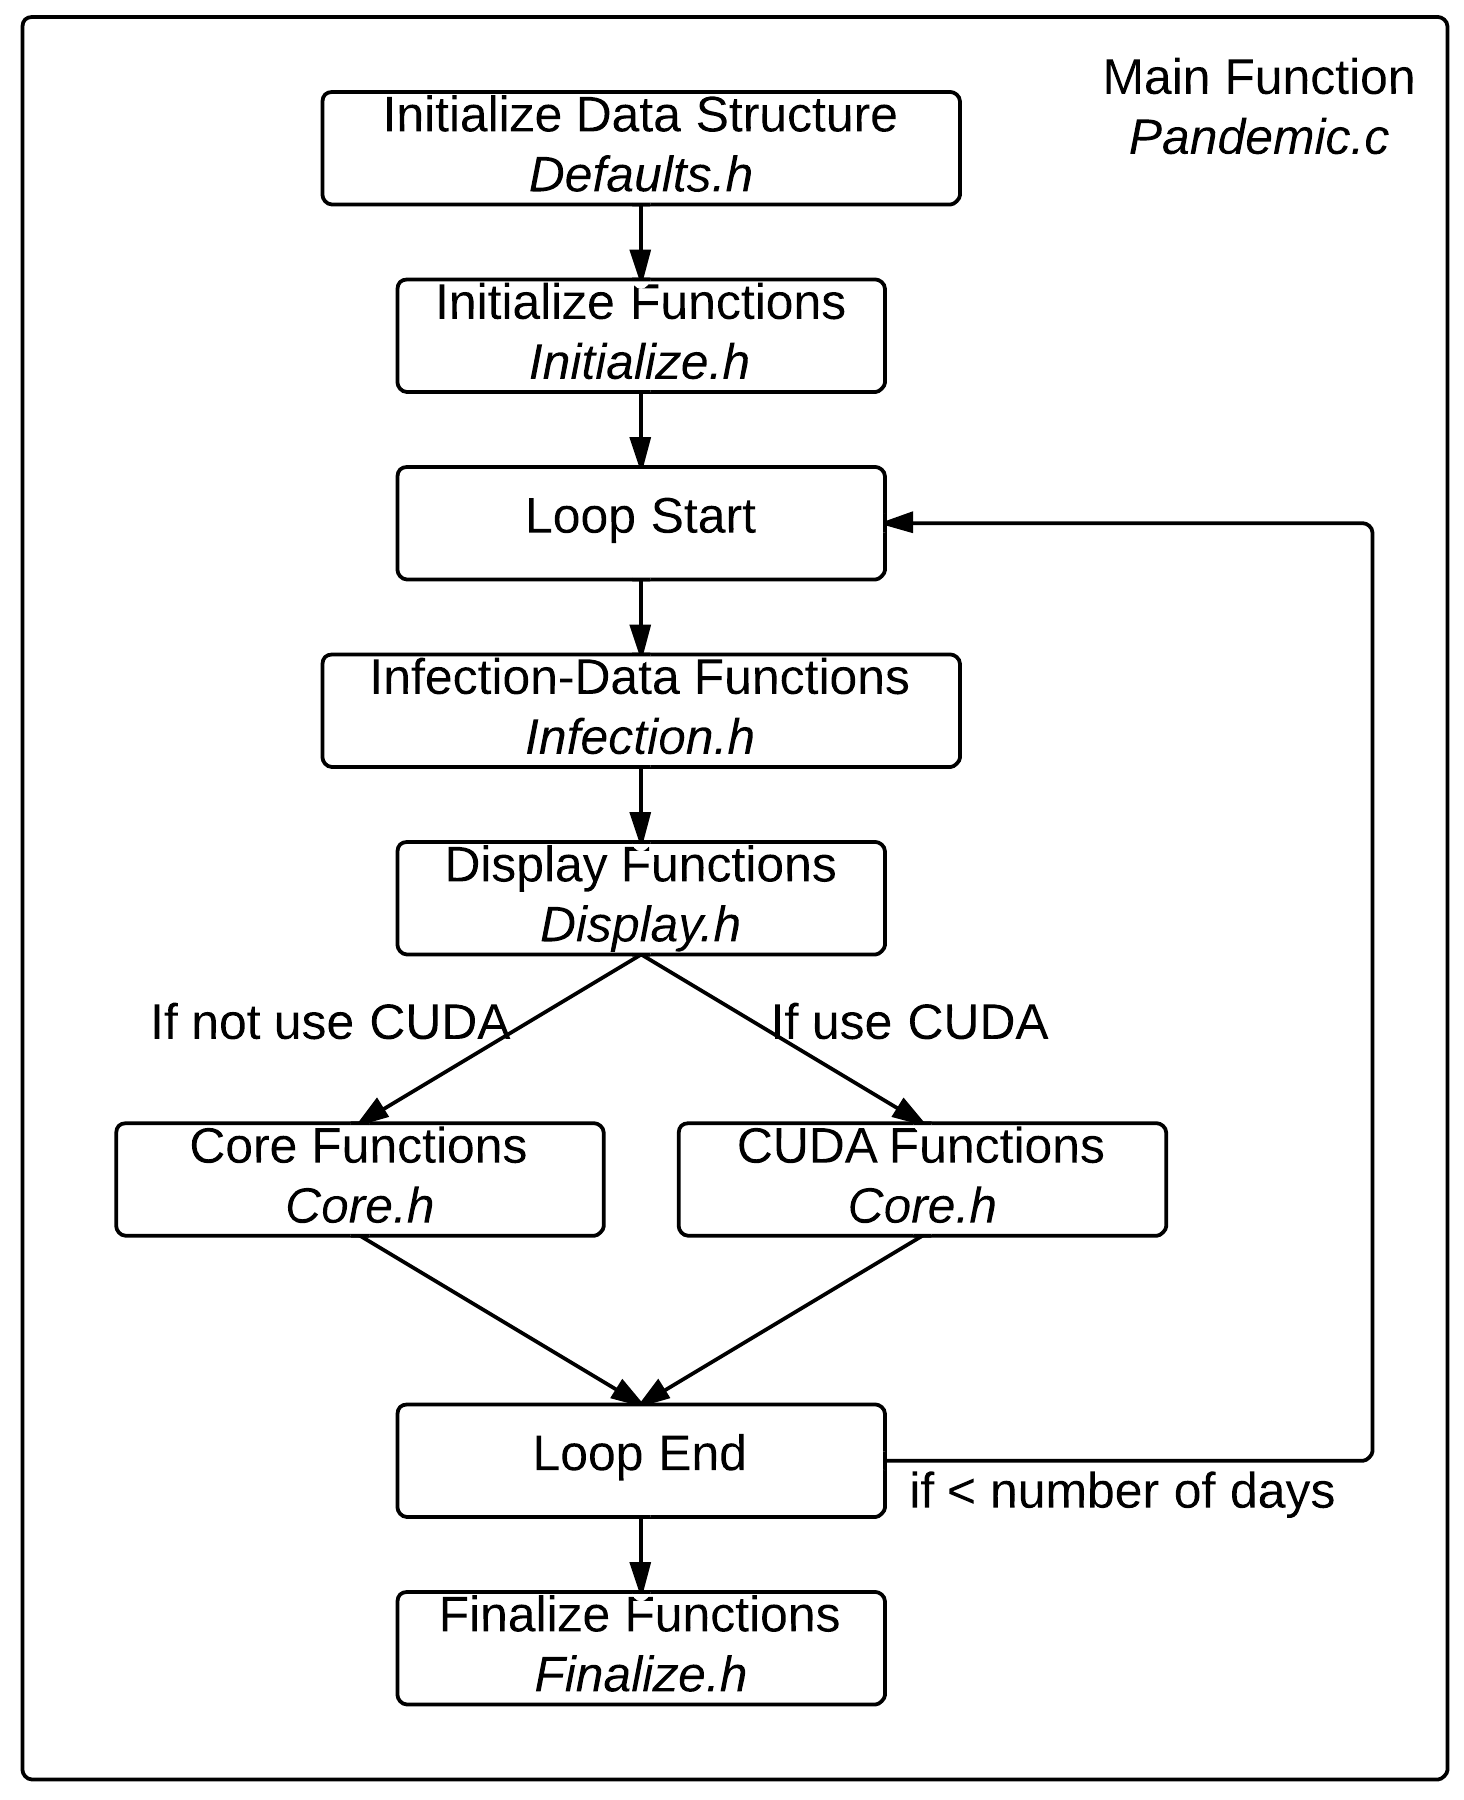
\includegraphics{Structure.png}
\caption{Overall Program Structurer}\end{figure}

The rest of the module will go through each of the code files. We can start with the \emph{Pandemic.c} file.


\section{Pandemic.c}
\label{1-ProgramStructure/programstructure:pandemic-c}
At the very beginning of the file, We first include four files that are needed for all versions.

\begin{Verbatim}[commandchars=\\\{\}]
\PYG{c+cp}{\PYGZsh{}}\PYG{c+cp}{include "Defaults.h"}
\PYG{c+cp}{\PYGZsh{}}\PYG{c+cp}{include "Initialize.h"}
\PYG{c+cp}{\PYGZsh{}}\PYG{c+cp}{include "Infection.h"}
\PYG{c+cp}{\PYGZsh{}}\PYG{c+cp}{include "Core.h"}
\PYG{c+cp}{\PYGZsh{}}\PYG{c+cp}{include "Finalize.h"}
\end{Verbatim}

Then, if we are using display, we include the display code file.

\begin{Verbatim}[commandchars=\\\{\}]
\PYG{c+cp}{\PYGZsh{}}\PYG{c+cp}{if defined(X\PYGZus{}DISPLAY) \textbar{}\textbar{} defined(TEXT\PYGZus{}DISPLAY)}
\PYG{c+cp}{\PYGZsh{}}\PYG{c+cp}{include "Display.h"}
\PYG{c+cp}{\PYGZsh{}}\PYG{c+cp}{endif}
\end{Verbatim}


\subsection{main()}
\label{1-ProgramStructure/programstructure:main}
This function is the backbone of the whole program. It first initialize all the data structures need.

\begin{Verbatim}[commandchars=\\\{\}]
    \PYG{c+cm}{/**** In Defaults.h ****/}
    \PYG{k}{struct} \PYG{n}{global\PYGZus{}t} \PYG{n}{global}\PYG{p}{;}
    \PYG{k}{struct} \PYG{n}{our\PYGZus{}t} \PYG{n}{our}\PYG{p}{;}
    \PYG{k}{struct} \PYG{n}{const\PYGZus{}t} \PYG{n}{constant}\PYG{p}{;}
    \PYG{k}{struct} \PYG{n}{stats\PYGZus{}t} \PYG{n}{stats}\PYG{p}{;}
    \PYG{k}{struct} \PYG{n}{display\PYGZus{}t} \PYG{n}{dpy}\PYG{p}{;}
    \PYG{c+cm}{/***********************/}
\end{Verbatim}

Then it will initialize the runtime environment by calling \textbf{init()} function.

\begin{Verbatim}[commandchars=\\\{\}]
    \PYG{c+cm}{/******************** In Initialize.h ********************/}
    \PYG{n}{init}\PYG{p}{(}\PYG{o}{\PYGZam{}}\PYG{n}{global}\PYG{p}{,} \PYG{o}{\PYGZam{}}\PYG{n}{our}\PYG{p}{,} \PYG{o}{\PYGZam{}}\PYG{n}{constant}\PYG{p}{,} \PYG{o}{\PYGZam{}}\PYG{n}{stats}\PYG{p}{,} \PYG{o}{\PYGZam{}}\PYG{n}{dpy}\PYG{p}{,} \PYG{o}{\PYGZam{}}\PYG{n}{argc}\PYG{p}{,} \PYG{o}{\PYGZam{}}\PYG{n}{argv}\PYG{p}{)}\PYG{p}{;}
    \PYG{c+cm}{/*********************************************************/}
\end{Verbatim}

Then we start the simulation. A for loop wraps around most of the functions, where the each iteration of the loop represents a day passing.

\begin{Verbatim}[commandchars=\\\{\}]
    \PYG{k}{for}\PYG{p}{(}\PYG{n}{our}\PYG{p}{.}\PYG{n}{current\PYGZus{}day} \PYG{o}{=} \PYG{l+m+mi}{0}\PYG{p}{;} \PYG{n}{our}\PYG{p}{.}\PYG{n}{current\PYGZus{}day} \PYG{o}{\PYGZlt{}}\PYG{o}{=} \PYG{n}{constant}\PYG{p}{.}\PYG{n}{total\PYGZus{}number\PYGZus{}of\PYGZus{}days}\PYG{p}{;} 
        \PYG{n}{our}\PYG{p}{.}\PYG{n}{current\PYGZus{}day}\PYG{o}{+}\PYG{o}{+}\PYG{p}{)}
    \PYG{p}{\PYGZob{}}
    \PYG{p}{\PYGZcb{}}
\end{Verbatim}

Inside the for loop, we first find all data related to the infection.

\begin{Verbatim}[commandchars=\\\{\}]
       \PYG{c+cm}{/****** In Infection.h ******/}
        \PYG{n}{find\PYGZus{}infected}\PYG{p}{(}\PYG{o}{\PYGZam{}}\PYG{n}{our}\PYG{p}{)}\PYG{p}{;}

        \PYG{n}{share\PYGZus{}infected}\PYG{p}{(}\PYG{o}{\PYGZam{}}\PYG{n}{global}\PYG{p}{,} \PYG{o}{\PYGZam{}}\PYG{n}{our}\PYG{p}{)}\PYG{p}{;}
        \PYG{c+cm}{/****************************/}
\end{Verbatim}

Then, if display is enabled, we display the infection status. In other words, we display everyone's location and their states of infection.

\begin{Verbatim}[commandchars=\\\{\}]
        \PYG{c+cm}{/**************** In Display.h *****************/}
        \PYG{c+cp}{\PYGZsh{}}\PYG{c+cp}{if defined(X\PYGZus{}DISPLAY) \textbar{}\textbar{} defined(TEXT\PYGZus{}DISPLAY)}

        \PYG{n}{share\PYGZus{}display\PYGZus{}info}\PYG{p}{(}\PYG{o}{\PYGZam{}}\PYG{n}{global}\PYG{p}{,} \PYG{o}{\PYGZam{}}\PYG{n}{our}\PYG{p}{)}\PYG{p}{;}

        \PYG{n}{do\PYGZus{}display}\PYG{p}{(}\PYG{o}{\PYGZam{}}\PYG{n}{global}\PYG{p}{,} \PYG{o}{\PYGZam{}}\PYG{n}{our}\PYG{p}{,} \PYG{o}{\PYGZam{}}\PYG{n}{constant}\PYG{p}{,} \PYG{o}{\PYGZam{}}\PYG{n}{dpy}\PYG{p}{)}\PYG{p}{;}

        \PYG{n}{throttle}\PYG{p}{(}\PYG{o}{\PYGZam{}}\PYG{n}{constant}\PYG{p}{)}\PYG{p}{;}
        
        \PYG{c+cp}{\PYGZsh{}}\PYG{c+cp}{endif}
        \PYG{c+cm}{/***********************************************/}
\end{Verbatim}

After display, we can call four core functions in \emph{Core.h*} code file.

\begin{Verbatim}[commandchars=\\\{\}]
        \PYG{c+cm}{/******************* In Core.h ******************/}
        \PYG{n}{move}\PYG{p}{(}\PYG{o}{\PYGZam{}}\PYG{n}{our}\PYG{p}{,} \PYG{o}{\PYGZam{}}\PYG{n}{constant}\PYG{p}{)}\PYG{p}{;}      

        \PYG{n}{susceptible}\PYG{p}{(}\PYG{o}{\PYGZam{}}\PYG{n}{global}\PYG{p}{,} \PYG{o}{\PYGZam{}}\PYG{n}{our}\PYG{p}{,} \PYG{o}{\PYGZam{}}\PYG{n}{constant}\PYG{p}{,} \PYG{o}{\PYGZam{}}\PYG{n}{stats}\PYG{p}{)}\PYG{p}{;}

        \PYG{n}{infected}\PYG{p}{(}\PYG{o}{\PYGZam{}}\PYG{n}{our}\PYG{p}{,} \PYG{o}{\PYGZam{}}\PYG{n}{constant}\PYG{p}{,} \PYG{o}{\PYGZam{}}\PYG{n}{stats}\PYG{p}{)}\PYG{p}{;}

        \PYG{n}{update\PYGZus{}days\PYGZus{}infected}\PYG{p}{(}\PYG{o}{\PYGZam{}}\PYG{n}{our}\PYG{p}{,} \PYG{o}{\PYGZam{}}\PYG{n}{constant}\PYG{p}{)}\PYG{p}{;}
        \PYG{c+cm}{/************************************************/}
\end{Verbatim}

This is the end of the loop.

Finally, after the loop, we can display the results and finalize the runtime environment.

\begin{Verbatim}[commandchars=\\\{\}]
    \PYG{c+cm}{/**************** In Finialize.h **************/}
    \PYG{n}{show\PYGZus{}results}\PYG{p}{(}\PYG{o}{\PYGZam{}}\PYG{n}{our}\PYG{p}{,} \PYG{o}{\PYGZam{}}\PYG{n}{stats}\PYG{p}{)}\PYG{p}{;}

    \PYG{n}{cleanup}\PYG{p}{(}\PYG{o}{\PYGZam{}}\PYG{n}{global}\PYG{p}{,} \PYG{o}{\PYGZam{}}\PYG{n}{our}\PYG{p}{,} \PYG{o}{\PYGZam{}}\PYG{n}{constant}\PYG{p}{,} \PYG{o}{\PYGZam{}}\PYG{n}{dpy}\PYG{p}{)}\PYG{p}{;}
    \PYG{c+cm}{/**********************************************/}
\end{Verbatim}


\chapter{Data Structures}
\label{2-DataStructure/datastructure:data-structures}\label{2-DataStructure/datastructure::doc}
Here is the list of variables and arrays used by the program. Note the
naming scheme; variables whose names begin with “my” are private to the
threads that use them. Variables whose names begin with “our” are
private to the processes that use them, but public to the threads within
that process. Variables are thus named from a thread’s perspective; “my”
variables are ones that I use, “our” variables are ones that I and the
other threads in my process use.


\section{global\_t struct}
\label{2-DataStructure/datastructure:global-t-struct}
\begin{Verbatim}[commandchars=\\\{\}]
\PYG{c+c1}{// All the data needed globally. Holds EVERYONE's location, }
\PYG{c+c1}{// states and other necessary counters.}
\PYG{k}{struct} \PYG{n}{global\PYGZus{}t} 
\PYG{p}{\PYGZob{}}
    \PYG{c+c1}{// people counters}
    \PYG{k+kt}{int} \PYG{n}{total\PYGZus{}number\PYGZus{}of\PYGZus{}people}\PYG{p}{;}
    \PYG{k+kt}{int} \PYG{n}{total\PYGZus{}num\PYGZus{}initially\PYGZus{}infected}\PYG{p}{;} 
    \PYG{k+kt}{int} \PYG{n}{total\PYGZus{}num\PYGZus{}infected}\PYG{p}{;}
    \PYG{c+c1}{// locations}
    \PYG{k+kt}{int} \PYG{o}{*}\PYG{n}{x\PYGZus{}locations}\PYG{p}{;}
    \PYG{k+kt}{int} \PYG{o}{*}\PYG{n}{y\PYGZus{}locations}\PYG{p}{;}
    \PYG{c+c1}{// infected people's locations}
    \PYG{k+kt}{int} \PYG{o}{*}\PYG{n}{their\PYGZus{}infected\PYGZus{}x\PYGZus{}locations}\PYG{p}{;}
    \PYG{k+kt}{int} \PYG{o}{*}\PYG{n}{their\PYGZus{}infected\PYGZus{}y\PYGZus{}locations}\PYG{p}{;}
    \PYG{c+c1}{// state}
    \PYG{k+kt}{char} \PYG{o}{*}\PYG{n}{states}\PYG{p}{;}
    \PYG{c+c1}{// MPI related}
    \PYG{k+kt}{int} \PYG{n}{total\PYGZus{}number\PYGZus{}of\PYGZus{}processes}\PYG{p}{;}
\PYG{p}{\PYGZcb{}}\PYG{p}{;}
\end{Verbatim}

\textbf{total\_number\_of\_people}

the total number of all people in the simulation; the sum of people assigned to each process. The value of this variable can be specified on the command line with the –n option.

\textbf{total\_num\_initially\_infected}

the total number of people who are initially infected; the sum of initially infected people assigned to each process. The value of this variable can be specified on the command line with the –i option. This is a subset of the total number of people, so the value of this variable must be smaller or equal to the value for \textbf{total\_number\_of\_people}.

\textbf{total\_num\_infected}

the total number of infected people; the sum of the number of infected people assigned to each process. This value changes throughout the course of the simulation.

\textbf{x\_locations}

array, holds the x locations of all of the people; only used if the environment needs to be displayed; otherwise, \textbf{our\_x\_locations} is used.

\textbf{y\_locations}

array, holds the y locations of all of the people; only used if the environment needs to be displayed; otherwise, \textbf{our\_y\_locations} is used.

\textbf{their\_infected\_x\_locations}

array, used in \textbf{susceptible()} function to keep track of the x locations of the infected people for which each process is responsible.

\textbf{their\_infected\_y\_locations}

array, used in step \textbf{susceptible()} function to keep track of the y locations of the infected people for which each process is responsible.

\textbf{states}

array, holds the states of all of the people; only used if the environment needs to be displayed; otherwise, \textbf{our\_states} is used.

\textbf{total\_number\_of\_processes}

used to keep track of how many processes are being used. If MPI is disabled, the value of this variable will be 1. If it is enabled, the value is set in \textbf{init()} function.


\section{our\_t struct}
\label{2-DataStructure/datastructure:our-t-struct}
\begin{Verbatim}[commandchars=\\\{\}]
\PYG{c+c1}{// All the data private to each node: Data being used by }
\PYG{c+c1}{// each process on a node in a cluster when using MPI.}
\PYG{c+c1}{// Each process holds data for location, states and }
\PYG{c+c1}{// other necessary counters for a subset of people.}
\PYG{k}{struct} \PYG{n}{our\PYGZus{}t} 
\PYG{p}{\PYGZob{}}
    \PYG{c+c1}{// current day}
    \PYG{k+kt}{int} \PYG{n}{current\PYGZus{}day}\PYG{p}{;}
    \PYG{c+c1}{// MPI related }
    \PYG{k+kt}{int} \PYG{n}{our\PYGZus{}rank}\PYG{p}{;}
    \PYG{c+c1}{// people counters}
    \PYG{k+kt}{int} \PYG{n}{our\PYGZus{}number\PYGZus{}of\PYGZus{}people}\PYG{p}{;}
    \PYG{k+kt}{int} \PYG{n}{our\PYGZus{}num\PYGZus{}initially\PYGZus{}infected}\PYG{p}{;}
    \PYG{c+c1}{// states counters}
    \PYG{k+kt}{int} \PYG{n}{our\PYGZus{}num\PYGZus{}infected}\PYG{p}{;}
    \PYG{k+kt}{int} \PYG{n}{our\PYGZus{}num\PYGZus{}susceptible}\PYG{p}{;}
    \PYG{k+kt}{int} \PYG{n}{our\PYGZus{}num\PYGZus{}immune}\PYG{p}{;}
    \PYG{k+kt}{int} \PYG{n}{our\PYGZus{}num\PYGZus{}dead}\PYG{p}{;} 
    \PYG{c+c1}{// our people's locations}
    \PYG{k+kt}{int} \PYG{o}{*}\PYG{n}{our\PYGZus{}x\PYGZus{}locations}\PYG{p}{;}
    \PYG{k+kt}{int} \PYG{o}{*}\PYG{n}{our\PYGZus{}y\PYGZus{}locations}\PYG{p}{;}
    \PYG{c+c1}{// our infected people's locations}
    \PYG{k+kt}{int} \PYG{o}{*}\PYG{n}{our\PYGZus{}infected\PYGZus{}x\PYGZus{}locations}\PYG{p}{;}
    \PYG{k+kt}{int} \PYG{o}{*}\PYG{n}{our\PYGZus{}infected\PYGZus{}y\PYGZus{}locations}\PYG{p}{;}
    \PYG{c+c1}{// our people's states}
    \PYG{k+kt}{char} \PYG{o}{*}\PYG{n}{our\PYGZus{}states}\PYG{p}{;}
    \PYG{c+c1}{// our people's infected time}
    \PYG{k+kt}{int} \PYG{o}{*}\PYG{n}{our\PYGZus{}num\PYGZus{}days\PYGZus{}infected}\PYG{p}{;}
\PYG{p}{\PYGZcb{}}\PYG{p}{;}
\end{Verbatim}

\textbf{our\_current\_day}

a loop iterator representing the ID of the current day being simulated by the current process.

\textbf{our\_rank}

used to keep track of the rank of the current process. If MPI is disabled, the value of this variable will be 0. If it is enabled, the value is set in \textbf{init()} function.

\textbf{our\_number\_of\_people}

the number of people for which the current process is responsible. This will be a number less than or equal to the total number of people. The value is determined in \textbf{find\_size()} function.

\textbf{our\_num\_initially\_infected}

the count of initially infected people for which the current process is responsible.

\textbf{our\_num\_infected}

a count of the number of infected people for which the current process is responsible.

\textbf{our\_num\_susceptible}

a count of the number of susceptible people for which the current process is responsible.

\textbf{our\_num\_immune}

a count of the number of immune people for which the current process is responsible.

\textbf{our\_num\_dead}

a count of the number of dead people for which the current process is responsible.

\textbf{our\_x\_locations}

array, holds the x locations of all the people for which the current process is responsible.

\textbf{our\_y\_locations}

array, holds the y locations of all the people for which the current process is responsible.

\textbf{our\_infected\_x\_locations}

array, holds the x locations of all the infected people for which the current process is responsible.

\textbf{our\_infected\_y\_locations}

array, holds the y locations of all the infected people for which the current process is responsible.

\textbf{our\_states}

array, holds the states of all the people for which the current process is responsible.

\textbf{our\_num\_days\_infected}

array, used to keep track of the number of days each person has been infected for which the current process is responsible.


\section{const\_t struct}
\label{2-DataStructure/datastructure:const-t-struct}
\begin{Verbatim}[commandchars=\\\{\}]
\PYG{c+c1}{// Data being used as constant}
\PYG{k}{struct} \PYG{n}{const\PYGZus{}t} 
\PYG{p}{\PYGZob{}}
    \PYG{c+c1}{// environment}
    \PYG{k+kt}{int} \PYG{n}{environment\PYGZus{}width}\PYG{p}{;}
    \PYG{k+kt}{int} \PYG{n}{environment\PYGZus{}height}\PYG{p}{;}
    \PYG{c+c1}{// disease}
    \PYG{k+kt}{int} \PYG{n}{infection\PYGZus{}radius}\PYG{p}{;}
    \PYG{k+kt}{int} \PYG{n}{duration\PYGZus{}of\PYGZus{}disease}\PYG{p}{;}
    \PYG{k+kt}{int} \PYG{n}{contagiousness\PYGZus{}factor}\PYG{p}{;}
    \PYG{k+kt}{int} \PYG{n}{deadliness\PYGZus{}factor}\PYG{p}{;}
    \PYG{c+c1}{// time}
    \PYG{k+kt}{int} \PYG{n}{total\PYGZus{}number\PYGZus{}of\PYGZus{}days}\PYG{p}{;}
    \PYG{k+kt}{int} \PYG{n}{microseconds\PYGZus{}per\PYGZus{}day}\PYG{p}{;}
\PYG{p}{\PYGZcb{}}\PYG{p}{;}
\end{Verbatim}

\textbf{environment\_width}

indicates how wide the environment is; used to draw the environment and to make sure people stay within the bounds of the environment.

\textbf{environment\_height}

indicates how high the environment is; used to draw the environment and to make sure people stay within the bounds of the environment.

\textbf{infection\_radius}

see the Introduction Chapter above. The value of this variable can be specified on the command line with the –d option.

\textbf{duration\_of\_disease}

see the Introduction Chapter above. The value of this variable can be specified on the command line with the –T option.

\textbf{contagiousness\_factor}

see the Introduction Chapter above. The value of this variable can be specified on the command line with the –c option.

\textbf{deadliness\_factor}

see the Introduction Chapter above. The value of this variable can be specified on the command line with the –D option.

\textbf{total\_number\_of\_days}

the total number of days over which to run the simulation.

\textbf{microseconds\_per\_day}

used to tell how many microseconds to freeze in between frames of animation. The value of this variable can be specified on the command line with the –m option.


\section{stats\_t struct}
\label{2-DataStructure/datastructure:stats-t-struct}
\begin{Verbatim}[commandchars=\\\{\}]
\PYG{c+c1}{// Stats data private to each node: Data being used by }
\PYG{c+c1}{// each process on a node in a cluster when using MPI. }
\PYG{c+c1}{// Each process holds stats data for a subset of people.}
\PYG{k}{struct} \PYG{n}{stats\PYGZus{}t} 
\PYG{p}{\PYGZob{}}
    \PYG{k+kt}{double} \PYG{n}{our\PYGZus{}num\PYGZus{}infections}\PYG{p}{;}
    \PYG{k+kt}{double} \PYG{n}{our\PYGZus{}num\PYGZus{}infection\PYGZus{}attempts}\PYG{p}{;}
    \PYG{k+kt}{double} \PYG{n}{our\PYGZus{}num\PYGZus{}deaths}\PYG{p}{;}
    \PYG{k+kt}{double} \PYG{n}{our\PYGZus{}num\PYGZus{}recovery\PYGZus{}attempts}\PYG{p}{;} 
\PYG{p}{\PYGZcb{}}\PYG{p}{;}
\end{Verbatim}

\textbf{our\_num\_infections}

used to count the number of actual infections that take place (in which an infected person transmits the disease to a susceptible person). Only used if the showing of results is enabled (i.e., if the program is to print out final results from the simulation). Used to determine the actual contagiousness of the disease, which can be compared to the contagiousness factor by the user.

\textbf{our\_num\_infection\_attempts}

used to count the number of times a susceptible person is within an infection radius of an infected person, even if the infection fails. Only used if the showing of results is enabled (i.e., if the program is to print out final results from the simulation). Used to determine the actual contagiousness of the disease, which can be compared to the contagiousness factor by the user.

\textbf{our\_num\_deaths}

used to count the number of times a person dies. Only used if the showing of results is enabled (i.e., if the program is to print out final results from the simulation). Used to determine the actual deadliness of the disease, which can be compared to the deadliness factor by the user.

\textbf{our\_num\_recovery\_attempts}

used to count the number of times an infected person is able to become immune. Only used if the showing of results is enabled (i.e., if the program is to print out final results from the simulation). Used to determine the actual deadliness of the disease, which can be compared to the deadliness factor by the user.


\section{display\_t struct}
\label{2-DataStructure/datastructure:display-t-struct}
\begin{Verbatim}[commandchars=\\\{\}]
\PYG{c+c1}{// Data being used for the X display}
\PYG{k}{struct} \PYG{n}{display\PYGZus{}t} 
\PYG{p}{\PYGZob{}}
    \PYG{c+cp}{\PYGZsh{}}\PYG{c+cp}{ifdef TEXT\PYGZus{}DISPLAY}
    \PYG{c+c1}{// Array of character arrays for text display }
    \PYG{k+kt}{char} \PYG{o}{*}\PYG{o}{*}\PYG{n}{environment}\PYG{p}{;}
    \PYG{c+cp}{\PYGZsh{}}\PYG{c+cp}{endif}

    \PYG{c+cp}{\PYGZsh{}}\PYG{c+cp}{ifdef X\PYGZus{}DISPLAY}
    \PYG{c+c1}{// Declare X-related variables }
    \PYG{n}{Display}         \PYG{o}{*}\PYG{n}{display}\PYG{p}{;}
    \PYG{n}{Window}          \PYG{n}{window}\PYG{p}{;}
    \PYG{k+kt}{int}             \PYG{n}{screen}\PYG{p}{;}
    \PYG{n}{Atom}            \PYG{n}{delete\PYGZus{}window}\PYG{p}{;}
    \PYG{n}{GC}              \PYG{n}{gc}\PYG{p}{;}
    \PYG{n}{XColor}          \PYG{n}{infected\PYGZus{}color}\PYG{p}{;}
    \PYG{n}{XColor}          \PYG{n}{immune\PYGZus{}color}\PYG{p}{;}
    \PYG{n}{XColor}          \PYG{n}{susceptible\PYGZus{}color}\PYG{p}{;}
    \PYG{n}{XColor}          \PYG{n}{dead\PYGZus{}color}\PYG{p}{;}
    \PYG{n}{Colormap}        \PYG{n}{colormap}\PYG{p}{;}
    \PYG{k+kt}{char}            \PYG{o}{*}\PYG{n}{red}\PYG{p}{;}
    \PYG{k+kt}{char}            \PYG{o}{*}\PYG{n}{green}\PYG{p}{;}
    \PYG{k+kt}{char}            \PYG{o}{*}\PYG{n}{black}\PYG{p}{;}
    \PYG{k+kt}{char}            \PYG{o}{*}\PYG{n}{white}\PYG{p}{;}
    \PYG{c+cp}{\PYGZsh{}}\PYG{c+cp}{endif}
\PYG{p}{\PYGZcb{}}\PYG{p}{;}
\end{Verbatim}

\textbf{environment}

2D array, holds an ASCII representation of the environment (see “state” under “Person” in the Introduction Chapter). This variable is used only when we are using Text Display.

\textbf{display}

Display, display pointer for the connection to the X server

\textbf{window}

Window, variable to holds the window id.

\textbf{screen}

Screen, variable to holds default screen

\textbf{delete\_window}

\textbf{gc}

\textbf{infected\_color}

\textbf{immune\_color}

\textbf{susceptible\_color}

\textbf{dead\_color}

\textbf{red}

array of char, holds value \#FF0000, which is the hex code for color red.

\textbf{green}

array of char, holds value \#00FF00, which is the hex code for color green.

\textbf{black}

array of char, holds value \#000000, which is the hex code for color black.

\textbf{white}

array of char, holds value \#FFFFFF, which is the hex code for color white.

\textbf{colormap}


\chapter{Initialize Functions}
\label{3-Initialize/initialize:initialize-functions}\label{3-Initialize/initialize::doc}

\section{init()}
\label{3-Initialize/initialize:init}
This function will first initialize variables in the constant structure with default values. It will also initialize \textbf{total\_number\_of\_people} variable, \textbf{total\_num\_initially\_infected} variable and \textbf{total\_num\_infected} variable. After this, it will set all the counters inside stats structure to zero, as well as state counters inside global struct.

Before executing the algorithm, the code starts by initializing MPI using

\begin{Verbatim}[commandchars=\\\{\}]
    \PYG{c+c1}{// Each process initializes the distributed memory environment}
    \PYG{n}{MPI\PYGZus{}Init}\PYG{p}{(}\PYG{o}{\PYGZam{}}\PYG{n}{argc}\PYG{p}{,} \PYG{o}{\PYGZam{}}\PYG{n}{argv}\PYG{p}{)}\PYG{p}{;}
\end{Verbatim}

We pass the addresses of the arguments to \textbf{main}, \textbf{argc} and \textbf{argv}, so that MPI can strip out anything from the command line related to MPI, such as \textbf{mpirun} or \textbf{–np}. \textbf{MPI\_Init} must be called before any other MPI functions are executed, and we also want to call it before we parse the rest of the command line arguments in \textbf{parse\_args()} function.
\begin{figure}[htbp]
\centering

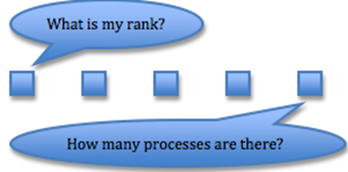
\includegraphics{img-51.png}
\end{figure}

Here we see one process figuring out its rank. It does so by calling

\begin{Verbatim}[commandchars=\\\{\}]
    \PYG{c+cp}{\PYGZsh{}}\PYG{c+cp}{ifdef \PYGZus{}MPI}
    \PYG{n}{MPI\PYGZus{}Comm\PYGZus{}rank}\PYG{p}{(}\PYG{n}{MPI\PYGZus{}COMM\PYGZus{}WORLD}\PYG{p}{,} \PYG{o}{\PYGZam{}}\PYG{n}{our}\PYG{o}{-}\PYG{o}{\PYGZgt{}}\PYG{n}{our\PYGZus{}rank}\PYG{p}{)}\PYG{p}{;}
\end{Verbatim}

function. This function checks the MPI “world” (the “communicator” of all the MPI processes, MPI\_COMM\_WORLD). You pass the address of the variable for the process’s rank to the function as the second argument using the ampersand (\&).

If we only have 1 process total (i.e., if we are not using distributed memory), then the rank of the process will be 0, which we set in the code as \textbf{our\_rank = 0}.

\begin{Verbatim}[commandchars=\\\{\}]
    \PYG{c+cp}{\PYGZsh{}}\PYG{c+cp}{else}
    \PYG{n}{our}\PYG{o}{-}\PYG{o}{\PYGZgt{}}\PYG{n}{our\PYGZus{}rank} \PYG{o}{=} \PYG{l+m+mi}{0}\PYG{p}{;}
\end{Verbatim}

We also see another process figuring out how many processes there are. It does so by calling

\begin{Verbatim}[commandchars=\\\{\}]
    \PYG{c+cp}{\PYGZsh{}}\PYG{c+cp}{ifdef \PYGZus{}MPI}
    \PYG{n}{MPI\PYGZus{}Comm\PYGZus{}size}\PYG{p}{(}\PYG{n}{MPI\PYGZus{}COMM\PYGZus{}WORLD}\PYG{p}{,} \PYG{o}{\PYGZam{}}\PYG{n}{global}\PYG{o}{-}\PYG{o}{\PYGZgt{}}\PYG{n}{total\PYGZus{}number\PYGZus{}of\PYGZus{}processes}\PYG{p}{)}\PYG{p}{;}
\end{Verbatim}

function. Just as with \textbf{MPI\_Comm\_rank}, you pass the communicator of all the processes and the address of the variable for the number of processes.

If we have only 1 process total, we set the number of processes by calling total\_number\_of\_processes = 1.

\begin{Verbatim}[commandchars=\\\{\}]
    \PYG{c+cp}{\PYGZsh{}}\PYG{c+cp}{else}
    \PYG{n}{global}\PYG{o}{-}\PYG{o}{\PYGZgt{}}\PYG{n}{total\PYGZus{}number\PYGZus{}of\PYGZus{}processes} \PYG{o}{=} \PYG{l+m+mi}{1}\PYG{p}{;}
\end{Verbatim}

After MPI initialization, \textbf{init()} function will call the following five functions.

\begin{Verbatim}[commandchars=\\\{\}]
    \PYG{n}{init\PYGZus{}check}\PYG{p}{(}\PYG{n}{global}\PYG{p}{)}\PYG{p}{;}
    \PYG{n}{parse\PYGZus{}args}\PYG{p}{(}\PYG{n}{global}\PYG{p}{,} \PYG{n}{constant}\PYG{p}{,} \PYG{n}{argc}\PYG{p}{,} \PYG{n}{argv}\PYG{p}{)}\PYG{p}{;}
    \PYG{n}{allocate\PYGZus{}array}\PYG{p}{(}\PYG{n}{global}\PYG{p}{,} \PYG{n}{our}\PYG{p}{,} \PYG{n}{constant}\PYG{p}{,} \PYG{n}{dpy}\PYG{p}{)}\PYG{p}{;}
    \PYG{n}{init\PYGZus{}array}\PYG{p}{(}\PYG{n}{our}\PYG{p}{,} \PYG{n}{constant}\PYG{p}{)}\PYG{p}{;}
    \PYG{c+c1}{// if use X\PYGZus{}DISPLAY, do init\PYGZus{}display()}
    \PYG{c+cp}{\PYGZsh{}}\PYG{c+cp}{ifdef X\PYGZus{}DISPLAY}
        \PYG{n}{init\PYGZus{}display}\PYG{p}{(}\PYG{n}{our}\PYG{p}{,} \PYG{n}{constant}\PYG{p}{,} \PYG{n}{dpy}\PYG{p}{)}\PYG{p}{;}
    \PYG{c+cp}{\PYGZsh{}}\PYG{c+cp}{endif}
\end{Verbatim}


\section{parse\_args()}
\label{3-Initialize/initialize:parse-args}\begin{figure}[htbp]
\centering

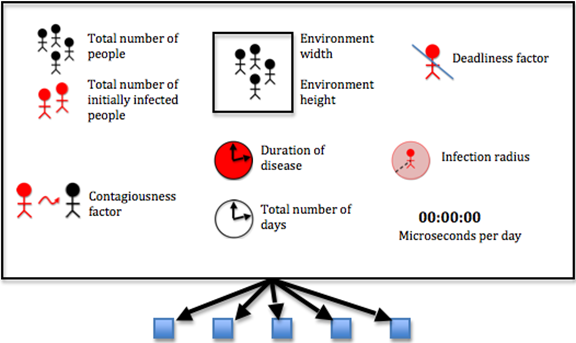
\includegraphics{img-6.png}
\end{figure}

These parameters are specified via command line arguments when the program is run. Otherwise, default values are used. The code uses \textbf{getopt} function to do this. Type \textbf{man 3 getopt} in a shell if you are interested how it works.


\section{init\_check()}
\label{3-Initialize/initialize:init-check}
This function makes sure that for each process, the total number of initially infected people is less than the total number of people
\begin{figure}[htbp]
\centering

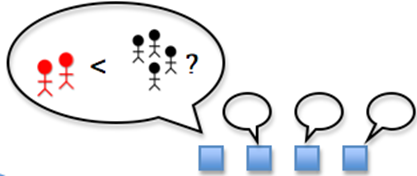
\includegraphics{img-7.png}
\end{figure}

The simulation can’t run if there are more initially infected people than there are people. If there are, the code uses the fprintf function to print an error message to standard error, and it exits the program with exit code -1.


\section{find\_size()}
\label{3-Initialize/initialize:find-size}
For each process, this function determines the number of people for which it is responsible
\begin{figure}[htbp]
\centering

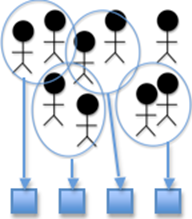
\includegraphics{img-8.png}
\end{figure}

Each process will try to take an even split of the number of people. It does so by dividing the number of people by the total number of processes and throwing away any remainder. Because the variables involved are integers in C, the throwing away of the remainder is handled automatically in the division

\begin{Verbatim}[commandchars=\\\{\}]
    \PYG{n}{our}\PYG{o}{-}\PYG{o}{\PYGZgt{}}\PYG{n}{our\PYGZus{}number\PYGZus{}of\PYGZus{}people} \PYG{o}{=} \PYG{n}{total\PYGZus{}number\PYGZus{}of\PYGZus{}people} \PYG{o}{/} \PYG{n}{total\PYGZus{}number\PYGZus{}of\PYGZus{}processes}\PYG{p}{;}
\end{Verbatim}

The last process is responsible for the remainder
\begin{figure}[htbp]
\centering

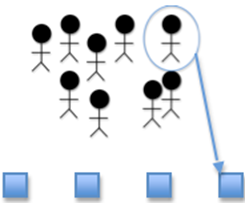
\includegraphics{img-9.png}
\end{figure}

\begin{Verbatim}[commandchars=\\\{\}]
    \PYG{c+c1}{// The last process is responsible for the remainder}
    \PYG{k}{if}\PYG{p}{(}\PYG{n}{our\PYGZus{}rank} \PYG{o}{=}\PYG{o}{=} \PYG{n}{total\PYGZus{}number\PYGZus{}of\PYGZus{}processes} \PYG{o}{-} \PYG{l+m+mi}{1}\PYG{p}{)}
    \PYG{p}{\PYGZob{}}
        \PYG{n}{our}\PYG{o}{-}\PYG{o}{\PYGZgt{}}\PYG{n}{our\PYGZus{}number\PYGZus{}of\PYGZus{}people} \PYG{o}{+}\PYG{o}{=} \PYG{n}{total\PYGZus{}number\PYGZus{}of\PYGZus{}people} \PYG{o}{\PYGZpc{}} \PYG{n}{total\PYGZus{}number\PYGZus{}of\PYGZus{}processes}\PYG{p}{;}
    \PYG{p}{\PYGZcb{}}
\end{Verbatim}

Every person has to be accounted for, so any remainder of the division is assigned to the last process. We can obtain the remainder by using the modulo operator (\%), and we add it to the existing value using the plus-equals operator (+=):

\begin{Verbatim}[commandchars=\\\{\}]
        \PYG{n}{our}\PYG{o}{-}\PYG{o}{\PYGZgt{}}\PYG{n}{our\PYGZus{}number\PYGZus{}of\PYGZus{}people} \PYG{o}{+}\PYG{o}{=} \PYG{n}{total\PYGZus{}number\PYGZus{}of\PYGZus{}people} \PYG{o}{\PYGZpc{}} \PYG{n}{total\PYGZus{}number\PYGZus{}of\PYGZus{}processes}\PYG{p}{;}
\end{Verbatim}

We only want the last process to do this, so we surround the code with

\begin{Verbatim}[commandchars=\\\{\}]
    \PYG{k}{if}\PYG{p}{(}\PYG{n}{our\PYGZus{}rank} \PYG{o}{=}\PYG{o}{=} \PYG{n}{total\PYGZus{}number\PYGZus{}of\PYGZus{}processes} \PYG{o}{-} \PYG{l+m+mi}{1}\PYG{p}{)}
\end{Verbatim}

since the last process has rank \textbf{N–1}, where N is the total number of processes.

Each process determines the number of initially infected people
for which it is responsible
\begin{figure}[htbp]
\centering

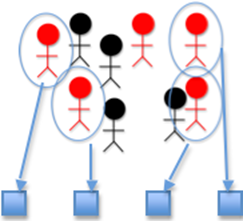
\includegraphics{img-10.png}
\end{figure}

\begin{Verbatim}[commandchars=\\\{\}]
    \PYG{n}{our}\PYG{o}{-}\PYG{o}{\PYGZgt{}}\PYG{n}{our\PYGZus{}num\PYGZus{}initially\PYGZus{}infected} \PYG{o}{=} \PYG{n}{total\PYGZus{}num\PYGZus{}initially\PYGZus{}infected} 
    \PYG{o}{/} \PYG{n}{total\PYGZus{}number\PYGZus{}of\PYGZus{}processes}\PYG{p}{;}
\end{Verbatim}

This is the same method used before, but it considers only the infected people.

The last process is responsible for the remainder
\begin{figure}[htbp]
\centering

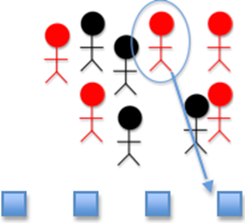
\includegraphics{img-11.png}
\end{figure}

\begin{Verbatim}[commandchars=\\\{\}]
        \PYG{n}{our}\PYG{o}{-}\PYG{o}{\PYGZgt{}}\PYG{n}{our\PYGZus{}num\PYGZus{}initially\PYGZus{}infected} \PYG{o}{+}\PYG{o}{=} \PYG{n}{total\PYGZus{}num\PYGZus{}initially\PYGZus{}infected} 
        \PYG{o}{\PYGZpc{}} \PYG{n}{total\PYGZus{}number\PYGZus{}of\PYGZus{}processes}\PYG{p}{;}
\end{Verbatim}

This is the same method used before, but it considers only the infected people.


\section{allocate\_array}
\label{3-Initialize/initialize:allocate-array}
At this point we are ready to allocate our arrays, which must be performed before we can start filling the arrays. Allocating an array means reserving enough space in memory for it; if we don’t reserve the space the program will assume that it is a zero-length array. The allocation must happen in the “heap” memory, meaning we must allocate it dynamically (i.e. as the program is running). To allocate memory on the heap, we use the \textbf{malloc} function, which takes the amount of space that is requested and returns a pointer to the newly allocated memory, which we can then use as an array. Let’s see an example with the x\_locations array:

\begin{Verbatim}[commandchars=\\\{\}]
    \PYG{n}{global}\PYG{o}{-}\PYG{o}{\PYGZgt{}}\PYG{n}{x\PYGZus{}locations} \PYG{o}{=} \PYG{p}{(}\PYG{k+kt}{int}\PYG{o}{*}\PYG{p}{)}\PYG{n}{malloc}\PYG{p}{(}\PYG{n}{total\PYGZus{}number\PYGZus{}of\PYGZus{}people} \PYG{o}{*} \PYG{k}{sizeof}\PYG{p}{(}\PYG{k+kt}{int}\PYG{p}{)}\PYG{p}{)}\PYG{p}{;}
\end{Verbatim}

Here we see that malloc has taken an argument, \textbf{total\_number\_of\_people * sizeof(int)}. This is how we specify that we want to fill the array with a certain number of integers, namely the amount stored in the \textbf{total\_number\_of\_people} variable. We also need to specify how big these integers are, for which we use the \textbf{sizeof(int)} function. We then take the return from \textbf{malloc} and tell the program to “cast” it (i.e. use it) as a pointer to integers, for which we use \textbf{(int*)}. This is then assigned to x\_locations, and we can now use \textbf{x\_locations} as an array.

For the 2D array \textbf{environment}, we must allocate not only the array itself but also each of the arrays that it contains (since a 2D array is an array whose elements are arrays). The array has horizontal strips of length \textbf{environment\_width} and vertical strips of length \textbf{environment\_height}. We perform the allocation by allocating enough space for the entire array first using

\begin{Verbatim}[commandchars=\\\{\}]
    \PYG{n}{dpy}\PYG{o}{-}\PYG{o}{\PYGZgt{}}\PYG{n}{environment} \PYG{o}{=} \PYG{p}{(}\PYG{k+kt}{char}\PYG{o}{*}\PYG{o}{*}\PYG{p}{)}\PYG{n}{malloc}\PYG{p}{(}\PYG{n}{constant}\PYG{o}{-}\PYG{o}{\PYGZgt{}}\PYG{n}{environment\PYGZus{}width} \PYG{o}{*} 
        \PYG{n}{constant}\PYG{o}{-}\PYG{o}{\PYGZgt{}}\PYG{n}{environment\PYGZus{}height} \PYG{o}{*} \PYG{k}{sizeof}\PYG{p}{(}\PYG{k+kt}{char}\PYG{o}{*}\PYG{p}{)}\PYG{p}{)}\PYG{p}{;}
\end{Verbatim}

That is, we are allocating enough \textbf{char*}’s for \textbf{environment\_width} times \textbf{environment\_height}, casting this as a \textbf{char**} and assigning it to \textbf{environment}. Then we allocate each array within \textbf{environment}, like so:

\begin{Verbatim}[commandchars=\\\{\}]
    \PYG{k}{for}\PYG{p}{(}\PYG{n}{our\PYGZus{}current\PYGZus{}location\PYGZus{}x} \PYG{o}{=} \PYG{l+m+mi}{0}\PYG{p}{;} 
        \PYG{n}{our\PYGZus{}current\PYGZus{}location\PYGZus{}x} \PYG{o}{\PYGZlt{}}\PYG{o}{=} \PYG{n}{constant}\PYG{o}{-}\PYG{o}{\PYGZgt{}}\PYG{n}{environment\PYGZus{}width} \PYG{o}{-} \PYG{l+m+mi}{1}\PYG{p}{;}
        \PYG{n}{our\PYGZus{}current\PYGZus{}location\PYGZus{}x}\PYG{o}{+}\PYG{o}{+}\PYG{p}{)}
    \PYG{p}{\PYGZob{}}
        \PYG{n}{dpy}\PYG{o}{-}\PYG{o}{\PYGZgt{}}\PYG{n}{environment}\PYG{p}{[}\PYG{n}{our\PYGZus{}current\PYGZus{}location\PYGZus{}x}\PYG{p}{]} \PYG{o}{=} \PYG{p}{(}\PYG{k+kt}{char}\PYG{o}{*}\PYG{p}{)}\PYG{n}{malloc}\PYG{p}{(}
            \PYG{n}{constant}\PYG{o}{-}\PYG{o}{\PYGZgt{}}\PYG{n}{environment\PYGZus{}height} \PYG{o}{*} \PYG{k}{sizeof}\PYG{p}{(}\PYG{k+kt}{char}\PYG{p}{)}\PYG{p}{)}\PYG{p}{;}
    \PYG{p}{\PYGZcb{}}
\end{Verbatim}

The number of arrays we need is stored in \textbf{environment\_width}, so we loop from \textbf{0} to \textbf{environment\_width – 1} and allocate enough space in each element of environment for \textbf{environment\_height} chars, each one of which has size \textbf{sizeof(char)}.

This can be a convoluted process but is necessary for allocating arrays dynamically, which allows us to specify options on the command line (so we don’t have to edit the source code and re-compile each time we want to run a simulation with different parameters).


\section{init\_array()}
\label{3-Initialize/initialize:init-array}
This function can be divided into four parts.

The function sets the states of the initially infected people and set the count of its infected people
\begin{figure}[htbp]
\centering

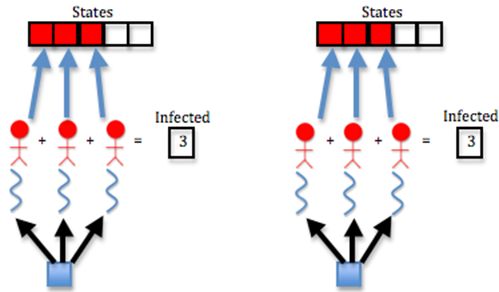
\includegraphics{img-12.png}
\end{figure}

The function also sets the states of infected people using the \textbf{our\_states} array. They fill the first \textbf{our\_num\_initially\_infected} cells of the array with the \textbf{INFECTED} constant; i.e. they fill in the \textbf{0} through \textbf{our\_num\_initially\_infected – 1} positions of the array with \textbf{INFECTED} as below:

\begin{Verbatim}[commandchars=\\\{\}]
    \PYG{c+c1}{// Each process spawns threads to set the states of the initially }
    \PYG{c+c1}{// infected people and set the count of its infected people}
    \PYG{k}{for}\PYG{p}{(}\PYG{n}{my\PYGZus{}current\PYGZus{}person\PYGZus{}id} \PYG{o}{=} \PYG{l+m+mi}{0}\PYG{p}{;} \PYG{n}{my\PYGZus{}current\PYGZus{}person\PYGZus{}id} 
        \PYG{o}{\PYGZlt{}}\PYG{o}{=} \PYG{n}{our\PYGZus{}num\PYGZus{}initially\PYGZus{}infected} \PYG{o}{-} \PYG{l+m+mi}{1}\PYG{p}{;} \PYG{n}{my\PYGZus{}current\PYGZus{}person\PYGZus{}id}\PYG{o}{+}\PYG{o}{+}\PYG{p}{)}
    \PYG{p}{\PYGZob{}}
        \PYG{n}{our}\PYG{o}{-}\PYG{o}{\PYGZgt{}}\PYG{n}{our\PYGZus{}states}\PYG{p}{[}\PYG{n}{my\PYGZus{}current\PYGZus{}person\PYGZus{}id}\PYG{p}{]} \PYG{o}{=} \PYG{n}{INFECTED}\PYG{p}{;}
        \PYG{n}{our}\PYG{o}{-}\PYG{o}{\PYGZgt{}}\PYG{n}{our\PYGZus{}num\PYGZus{}infected}\PYG{o}{+}\PYG{o}{+}\PYG{p}{;}
    \PYG{p}{\PYGZcb{}}
\end{Verbatim}

The function sets the states of the rest of its
people and set the count of its susceptible people
\begin{figure}[htbp]
\centering

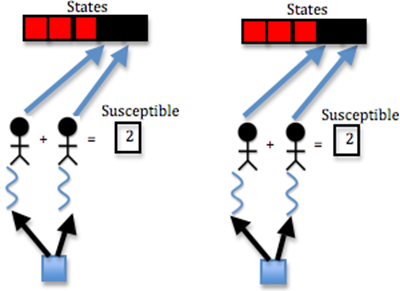
\includegraphics{img-13.png}
\end{figure}

This is similar to last step, but we want to fill the rest of the array (from \textbf{our\_num\_initially\_infected} to \textbf{our\_number\_of\_people - 1}) with the \textbf{SUSCEPTIBLE} constant, and we want to add \textbf{1} to the \textbf{our\_num\_susceptible} variable at each iteration of the loop:

\begin{Verbatim}[commandchars=\\\{\}]
    \PYG{c+c1}{// Each process spawns threads to set the states of the rest of}
    \PYG{c+c1}{// its people and set the count of its susceptible people}
    \PYG{k}{for}\PYG{p}{(}\PYG{n}{my\PYGZus{}current\PYGZus{}person\PYGZus{}id} \PYG{o}{=} \PYG{n}{our\PYGZus{}num\PYGZus{}initially\PYGZus{}infected}\PYG{p}{;} 
        \PYG{n}{my\PYGZus{}current\PYGZus{}person\PYGZus{}id} \PYG{o}{\PYGZlt{}}\PYG{o}{=} \PYG{n}{our\PYGZus{}number\PYGZus{}of\PYGZus{}people} \PYG{o}{-} \PYG{l+m+mi}{1}\PYG{p}{;} 
        \PYG{n}{my\PYGZus{}current\PYGZus{}person\PYGZus{}id}\PYG{o}{+}\PYG{o}{+}\PYG{p}{)}
    \PYG{p}{\PYGZob{}}
        \PYG{n}{our}\PYG{o}{-}\PYG{o}{\PYGZgt{}}\PYG{n}{our\PYGZus{}states}\PYG{p}{[}\PYG{n}{my\PYGZus{}current\PYGZus{}person\PYGZus{}id}\PYG{p}{]} \PYG{o}{=} \PYG{n}{SUSCEPTIBLE}\PYG{p}{;}
        \PYG{n}{our}\PYG{o}{-}\PYG{o}{\PYGZgt{}}\PYG{n}{our\PYGZus{}num\PYGZus{}susceptible}\PYG{o}{+}\PYG{o}{+}\PYG{p}{;}
    \PYG{p}{\PYGZcb{}}
\end{Verbatim}

The \textbf{our\_states} array is now full; the first \textbf{our\_num\_initially\_infected} cells have the \textbf{INFECTED} constant, and the rest have the \textbf{SUSCEPTIBLE} constant.

The third step is that the function sets random x and y locations for each of its people
\begin{figure}[htbp]
\centering

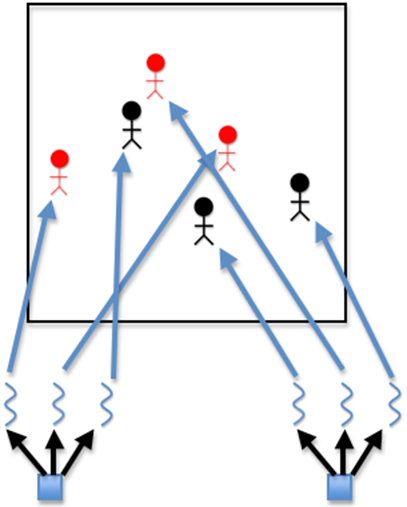
\includegraphics{img-14.png}
\end{figure}

Locations of people are stored in the \textbf{our\_x\_locations} and \textbf{our\_y\_locations} arrays. To fill these arrays with random values, we use a for loop and the random function:

\begin{Verbatim}[commandchars=\\\{\}]
    \PYG{c+c1}{// Each process spawns threads to set random x and y locations for }
    \PYG{c+c1}{// each of its people}
    \PYG{k}{for}\PYG{p}{(}\PYG{n}{my\PYGZus{}current\PYGZus{}person\PYGZus{}id} \PYG{o}{=} \PYG{l+m+mi}{0}\PYG{p}{;}
        \PYG{n}{my\PYGZus{}current\PYGZus{}person\PYGZus{}id} \PYG{o}{\PYGZlt{}}\PYG{o}{=} \PYG{n}{our\PYGZus{}number\PYGZus{}of\PYGZus{}people} \PYG{o}{-} \PYG{l+m+mi}{1}\PYG{p}{;} 
        \PYG{n}{my\PYGZus{}current\PYGZus{}person\PYGZus{}id}\PYG{o}{+}\PYG{o}{+}\PYG{p}{)}
    \PYG{p}{\PYGZob{}}
        \PYG{n}{our}\PYG{o}{-}\PYG{o}{\PYGZgt{}}\PYG{n}{our\PYGZus{}x\PYGZus{}locations}\PYG{p}{[}\PYG{n}{my\PYGZus{}current\PYGZus{}person\PYGZus{}id}\PYG{p}{]} \PYG{o}{=} \PYG{n}{random}\PYG{p}{(}\PYG{p}{)} \PYG{o}{\PYGZpc{}} \PYG{n}{constant}\PYG{o}{-}\PYG{o}{\PYGZgt{}}\PYG{n}{environment\PYGZus{}width}\PYG{p}{;}
        \PYG{n}{our}\PYG{o}{-}\PYG{o}{\PYGZgt{}}\PYG{n}{our\PYGZus{}y\PYGZus{}locations}\PYG{p}{[}\PYG{n}{my\PYGZus{}current\PYGZus{}person\PYGZus{}id}\PYG{p}{]} \PYG{o}{=} \PYG{n}{random}\PYG{p}{(}\PYG{p}{)} \PYG{o}{\PYGZpc{}} \PYG{n}{constant}\PYG{o}{-}\PYG{o}{\PYGZgt{}}\PYG{n}{environment\PYGZus{}height}\PYG{p}{;}
    \PYG{p}{\PYGZcb{}}
\end{Verbatim}

By calling random with the \textbf{modulus (\%)} operator, we can restrict the size of the random number it generates. Since we cannot have x locations larger than the width of the environment, we call \textbf{random() \% environment\_width}; to make sure the \textbf{x location} of each person is less than \textbf{environment\_width}. Similarly for the \textbf{y location} and \textbf{environment\_height}.

We are filling the x and y location arrays for all of the people for which the process is responsible, so we loop from \textbf{0} to \textbf{our\_number\_of\_people – 1}.

Finally, the function initializes the number of days infected of each of its people to 0
\begin{figure}[htbp]
\centering

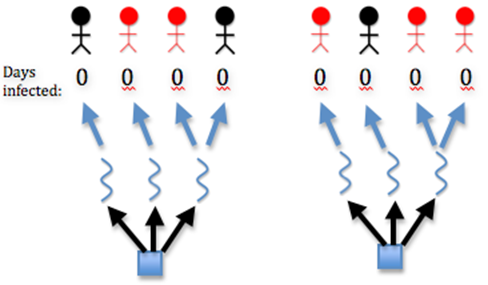
\includegraphics{img-15.png}
\end{figure}

The number of days each person is infected is stored in the \textbf{our\_num\_days\_infected} array, so we loop over all of the people and fill this array with 0, since the simulation starts at day 0, at which point no days have yet elapsed:

\begin{Verbatim}[commandchars=\\\{\}]
    \PYG{c+c1}{// Each process spawns threads to initialize the number of days }
    \PYG{c+c1}{// infected of each of its people to 0}
    \PYG{k}{for}\PYG{p}{(}\PYG{n}{my\PYGZus{}current\PYGZus{}person\PYGZus{}id} \PYG{o}{=} \PYG{l+m+mi}{0}\PYG{p}{;}
        \PYG{n}{my\PYGZus{}current\PYGZus{}person\PYGZus{}id} \PYG{o}{\PYGZlt{}}\PYG{o}{=} \PYG{n}{our\PYGZus{}number\PYGZus{}of\PYGZus{}people} \PYG{o}{-} \PYG{l+m+mi}{1}\PYG{p}{;}
        \PYG{n}{my\PYGZus{}current\PYGZus{}person\PYGZus{}id}\PYG{o}{+}\PYG{o}{+}\PYG{p}{)}
    \PYG{p}{\PYGZob{}}
        \PYG{n}{our}\PYG{o}{-}\PYG{o}{\PYGZgt{}}\PYG{n}{our\PYGZus{}num\PYGZus{}days\PYGZus{}infected}\PYG{p}{[}\PYG{n}{my\PYGZus{}current\PYGZus{}person\PYGZus{}id}\PYG{p}{]} \PYG{o}{=} \PYG{l+m+mi}{0}\PYG{p}{;}
    \PYG{p}{\PYGZcb{}}
\end{Verbatim}


\chapter{Infection Functions}
\label{4-Infection/infection:infection-functions}\label{4-Infection/infection::doc}

\section{find\_infected}
\label{4-Infection/infection:find-infected}
For each process, this function determines its infected x locations and infected y locations
\begin{figure}[htbp]
\centering

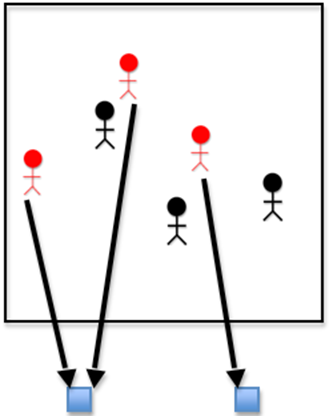
\includegraphics{img-16.png}
\end{figure}

We have already set the states of the infected people and the positions of all the people, but we need to specifically set the positions of the infected people and store them in the \textbf{our\_infected\_x\_locations} and \textbf{our\_infected\_y\_locations} arrays. We do this by marching through the \textbf{our\_states} array and checking whether the state at each cell is \textbf{INFECTED}. If it is, we add the locations of the current infected person from the \textbf{our\_x\_locations} and \textbf{our\_y\_locations} arrays to the \textbf{our\_infected\_x\_locations} and \textbf{our\_infected\_y\_locations} arrays. We determine the ID of the current infected person using the \textbf{our\_current\_infected\_person} variable:

\begin{Verbatim}[commandchars=\\\{\}]
    \PYG{k}{for}\PYG{p}{(}\PYG{n}{our\PYGZus{}person1} \PYG{o}{=} \PYG{l+m+mi}{0}\PYG{p}{;} \PYG{n}{our\PYGZus{}person1} \PYG{o}{\PYGZlt{}}\PYG{o}{=} \PYG{n}{our}\PYG{o}{-}\PYG{o}{\PYGZgt{}}\PYG{n}{our\PYGZus{}number\PYGZus{}of\PYGZus{}people} \PYG{o}{-} \PYG{l+m+mi}{1}\PYG{p}{;} \PYG{n}{our\PYGZus{}person1}\PYG{o}{+}\PYG{o}{+}\PYG{p}{)}
    \PYG{p}{\PYGZob{}}
        \PYG{k}{if}\PYG{p}{(}\PYG{n}{our}\PYG{o}{-}\PYG{o}{\PYGZgt{}}\PYG{n}{our\PYGZus{}states}\PYG{p}{[}\PYG{n}{our\PYGZus{}person1}\PYG{p}{]} \PYG{o}{=}\PYG{o}{=} \PYG{n}{INFECTED}\PYG{p}{)}
        \PYG{p}{\PYGZob{}}
            \PYG{n}{our}\PYG{o}{-}\PYG{o}{\PYGZgt{}}\PYG{n}{our\PYGZus{}infected\PYGZus{}x\PYGZus{}locations}\PYG{p}{[}\PYG{n}{our\PYGZus{}current\PYGZus{}infected\PYGZus{}person}\PYG{p}{]} \PYG{o}{=} 
            \PYG{n}{our}\PYG{o}{-}\PYG{o}{\PYGZgt{}}\PYG{n}{our\PYGZus{}x\PYGZus{}locations}\PYG{p}{[}\PYG{n}{our\PYGZus{}person1}\PYG{p}{]}\PYG{p}{;}
            \PYG{n}{our}\PYG{o}{-}\PYG{o}{\PYGZgt{}}\PYG{n}{our\PYGZus{}infected\PYGZus{}y\PYGZus{}locations}\PYG{p}{[}\PYG{n}{our\PYGZus{}current\PYGZus{}infected\PYGZus{}person}\PYG{p}{]} \PYG{o}{=}
            \PYG{n}{our}\PYG{o}{-}\PYG{o}{\PYGZgt{}}\PYG{n}{our\PYGZus{}y\PYGZus{}locations}\PYG{p}{[}\PYG{n}{our\PYGZus{}person1}\PYG{p}{]}\PYG{p}{;}
            \PYG{n}{our\PYGZus{}current\PYGZus{}infected\PYGZus{}person}\PYG{o}{+}\PYG{o}{+}\PYG{p}{;}
        \PYG{p}{\PYGZcb{}}
    \PYG{p}{\PYGZcb{}}
\end{Verbatim}


\section{share\_infected}
\label{4-Infection/infection:share-infected}
First, for each process, this function sends its count of infected people to all the other processes and receives their counts
\begin{figure}[htbp]
\centering

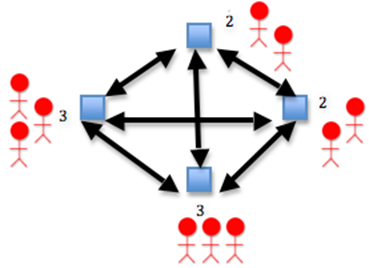
\includegraphics{img-17.png}
\end{figure}

\begin{Verbatim}[commandchars=\\\{\}]
    \PYG{c+c1}{// Each process sends its count of infected people to all the}
    \PYG{c+c1}{// other processes and receives their counts}
    \PYG{n}{MPI\PYGZus{}Allgather}\PYG{p}{(}\PYG{o}{\PYGZam{}}\PYG{n}{our}\PYG{o}{-}\PYG{o}{\PYGZgt{}}\PYG{n}{our\PYGZus{}num\PYGZus{}infected}\PYG{p}{,} \PYG{l+m+mi}{1}\PYG{p}{,} \PYG{n}{MPI\PYGZus{}INT}\PYG{p}{,} \PYG{n}{recvcounts}\PYG{p}{,} \PYG{l+m+mi}{1}\PYG{p}{,} 
        \PYG{n}{MPI\PYGZus{}INT}\PYG{p}{,} \PYG{n}{MPI\PYGZus{}COMM\PYGZus{}WORLD}\PYG{p}{)}\PYG{p}{;}
\end{Verbatim}

This step is handled by the MPI command \textbf{MPI\_Allgather} whose arguments are as follows:
\begin{itemize}
\item {} 
\textbf{\&our\_num\_infected} – the address of the sending buffer (the thing being sent).

\item {} 
\textbf{1} – the count of things being sent.

\item {} 
\textbf{MPI\_INT} – the datatype of things being sent.

\item {} 
\textbf{recvcounts} – the receive buffer (an array of things being received).

\item {} 
\textbf{1} – the count of things being received.

\item {} 
\textbf{MPI\_INT} – the datatype of things being received.

\item {} 
\textbf{MPI\_COMM\_WORLD} – the communicator of processes that send and receive data.

\end{itemize}

Once the data has been sent and received, we count the total number of infected people by adding up the values in the \textbf{recvcounts} array and storing the result in the \textbf{total\_num\_infected} variable:

\begin{Verbatim}[commandchars=\\\{\}]
    \PYG{n}{global}\PYG{o}{-}\PYG{o}{\PYGZgt{}}\PYG{n}{total\PYGZus{}num\PYGZus{}infected} \PYG{o}{=} \PYG{l+m+mi}{0}\PYG{p}{;}
    \PYG{k+kt}{int} \PYG{n}{current\PYGZus{}rank}\PYG{p}{;}
    \PYG{k}{for}\PYG{p}{(}\PYG{n}{current\PYGZus{}rank} \PYG{o}{=} \PYG{l+m+mi}{0}\PYG{p}{;} \PYG{n}{current\PYGZus{}rank} \PYG{o}{\PYGZlt{}}\PYG{o}{=} \PYG{n}{total\PYGZus{}number\PYGZus{}of\PYGZus{}processes} \PYG{o}{-} \PYG{l+m+mi}{1}\PYG{p}{;}
        \PYG{n}{current\PYGZus{}rank}\PYG{o}{+}\PYG{o}{+}\PYG{p}{)}
    \PYG{p}{\PYGZob{}}
        \PYG{n}{global}\PYG{o}{-}\PYG{o}{\PYGZgt{}}\PYG{n}{total\PYGZus{}num\PYGZus{}infected} \PYG{o}{+}\PYG{o}{=} \PYG{n}{recvcounts}\PYG{p}{[}\PYG{n}{current\PYGZus{}rank}\PYG{p}{]}\PYG{p}{;}
    \PYG{p}{\PYGZcb{}}
\end{Verbatim}

Next, for each process, the function sends the x locations of its infected people to all the other processes and receives the x locations of their infected people

For this send and receive, we need to use \textbf{MPI\_Allgatherv} instead of \textbf{MPI\_Allgather}. This is because each process has a varying number of infected people, so it needs to be able to send a variable number of x locations. To do this, we first need to set up the displacements in the receive buffer; that is, we need to indicate how many elements each process will send and at what points in the receive array they will appear. We can do this with a \textbf{displs} array, which will contain a list of the displacements in the receive buffer:

\begin{Verbatim}[commandchars=\\\{\}]
    \PYG{c+c1}{// Each process sends the x locations of its infected people to }
    \PYG{c+c1}{// all the other processes and receives the x locations of their }
    \PYG{c+c1}{// infected people}
    \PYG{n}{MPI\PYGZus{}Allgatherv}\PYG{p}{(}\PYG{n}{our}\PYG{o}{-}\PYG{o}{\PYGZgt{}}\PYG{n}{our\PYGZus{}infected\PYGZus{}x\PYGZus{}locations}\PYG{p}{,} \PYG{n}{our}\PYG{o}{-}\PYG{o}{\PYGZgt{}}\PYG{n}{our\PYGZus{}num\PYGZus{}infected}\PYG{p}{,} \PYG{n}{MPI\PYGZus{}INT}\PYG{p}{,} 
        \PYG{n}{global}\PYG{o}{-}\PYG{o}{\PYGZgt{}}\PYG{n}{their\PYGZus{}infected\PYGZus{}x\PYGZus{}locations}\PYG{p}{,} \PYG{n}{recvcounts}\PYG{p}{,} \PYG{n}{displs}\PYG{p}{,} 
        \PYG{n}{MPI\PYGZus{}INT}\PYG{p}{,} \PYG{n}{MPI\PYGZus{}COMM\PYGZus{}WORLD}\PYG{p}{)}\PYG{p}{;}
\end{Verbatim}

We are now ready to call the \textbf{MPI\_Allgatherv}. Here are its arguments:
\begin{itemize}
\item {} 
\textbf{our\_infected\_x\_locations} – the send buffer (array of things to send).

\item {} 
\textbf{our\_num\_infected} – the count of elements in the send buffer.

\item {} 
\textbf{MPI\_INT} – the datatype of the elements in the send buffer.

\item {} 
\textbf{their\_infected\_x\_locations} – the receive buffer (array of things to receive).

\item {} 
\textbf{recvcounts} – an array of counts of elements in the receive buffer

\item {} 
\textbf{displs} – the list of displacements in the receive buffer, as determined above.

\item {} 
\textbf{MPI\_INT} – the data type of the elements in the receive buffer.

\item {} 
\textbf{MPI\_COMM\_WORLD} – the communicator of processes that send and receive data.

\end{itemize}

Once the command is complete, each process will have the full array of the x locations of the infected people from each process, stored in the \textbf{their\_infected\_x\_locations} array.

Finally, each process sends the y locations of its infected people to all the other processes and receives the y locations of their infected people

\begin{Verbatim}[commandchars=\\\{\}]
    \PYG{c+c1}{// Each process sends the y locations of its infected people }
    \PYG{c+c1}{// to all the other processes and receives the y locations of their }
    \PYG{c+c1}{// infected people}
    \PYG{n}{MPI\PYGZus{}Allgatherv}\PYG{p}{(}\PYG{n}{our}\PYG{o}{-}\PYG{o}{\PYGZgt{}}\PYG{n}{our\PYGZus{}infected\PYGZus{}y\PYGZus{}locations}\PYG{p}{,} \PYG{n}{our}\PYG{o}{-}\PYG{o}{\PYGZgt{}}\PYG{n}{our\PYGZus{}num\PYGZus{}infected}\PYG{p}{,} \PYG{n}{MPI\PYGZus{}INT}\PYG{p}{,} 
        \PYG{n}{global}\PYG{o}{-}\PYG{o}{\PYGZgt{}}\PYG{n}{their\PYGZus{}infected\PYGZus{}y\PYGZus{}locations}\PYG{p}{,} \PYG{n}{recvcounts}\PYG{p}{,} \PYG{n}{displs}\PYG{p}{,} 
        \PYG{n}{MPI\PYGZus{}INT}\PYG{p}{,} \PYG{n}{MPI\PYGZus{}COMM\PYGZus{}WORLD}\PYG{p}{)}\PYG{p}{;}
\end{Verbatim}

The y locations are sent and received just as the x locations are sent and received. In fact, the function calls have exactly 2 letters difference; the x’s in the \textbf{Allgatherv} from last step. are replaced by y’s in the \textbf{Allgatherv} in this step.

Note that the code will only execute previous two steps if MPI is enabled. If it is not enabled, the code simply copies the \textbf{our\_infected\_x\_locations} and \textbf{our\_infected\_y\_locations} arrays into the \textbf{their\_infected\_x\_locations} and \textbf{their\_infected\_y\_locations} arrays and the \textbf{our\_num\_infected} variable into the \textbf{total\_num\_infected} variable.


\chapter{Display Functions}
\label{5-Display/display::doc}\label{5-Display/display:display-functions}

\section{init\_display}
\label{5-Display/display:init-display}
Rank 0 initializes the graphics display. The code uses X to handle graphics display.


\section{share\_location}
\label{5-Display/display:share-location}
If display is enabled, Rank 0 gathers the states, x locations, and y locations of the people for which each process is responsible
\begin{figure}[htbp]
\centering

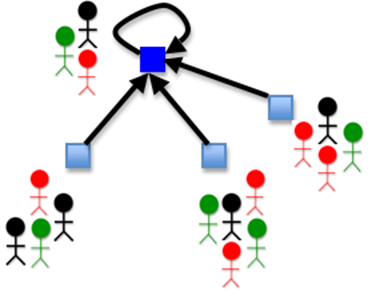
\includegraphics{img-18.png}
\end{figure}

We set up the displs here just as we did in function \textbf{share\_infected()}.

\begin{Verbatim}[commandchars=\\\{\}]
    \PYG{c+c1}{// Distributed Memory Information}
    \PYG{k+kt}{int} \PYG{o}{*}\PYG{n}{recvcounts}\PYG{p}{;}
    \PYG{k+kt}{int} \PYG{o}{*}\PYG{n}{displs}\PYG{p}{;}
    \PYG{n}{recvcounts} \PYG{o}{=} \PYG{p}{(}\PYG{k+kt}{int}\PYG{o}{*}\PYG{p}{)}\PYG{n}{malloc}\PYG{p}{(}\PYG{n}{total\PYGZus{}number\PYGZus{}of\PYGZus{}processes} \PYG{o}{*} \PYG{k}{sizeof}\PYG{p}{(}\PYG{k+kt}{int}\PYG{p}{)}\PYG{p}{)}\PYG{p}{;}  
    \PYG{n}{displs} \PYG{o}{=} \PYG{p}{(}\PYG{k+kt}{int}\PYG{o}{*}\PYG{p}{)}\PYG{n}{malloc}\PYG{p}{(}\PYG{n}{total\PYGZus{}number\PYGZus{}of\PYGZus{}processes} \PYG{o}{*} \PYG{k}{sizeof}\PYG{p}{(}\PYG{k+kt}{int}\PYG{p}{)}\PYG{p}{)}\PYG{p}{;}

    \PYG{c+c1}{// Set up the receive counts and displacements in the }
    \PYG{c+c1}{// receive buffer (see the man page for MPI\PYGZus{}Gatherv)}
    \PYG{k+kt}{int} \PYG{n}{current\PYGZus{}displ} \PYG{o}{=} \PYG{l+m+mi}{0}\PYG{p}{;}
    \PYG{k+kt}{int} \PYG{n}{current\PYGZus{}rank}\PYG{p}{;}
    \PYG{k}{for}\PYG{p}{(}\PYG{n}{current\PYGZus{}rank} \PYG{o}{=} \PYG{l+m+mi}{0}\PYG{p}{;} \PYG{n}{current\PYGZus{}rank} \PYG{o}{\PYGZlt{}}\PYG{o}{=} \PYG{n}{total\PYGZus{}number\PYGZus{}of\PYGZus{}processes} \PYG{o}{-} \PYG{l+m+mi}{1}\PYG{p}{;}
       \PYG{n}{current\PYGZus{}rank}\PYG{o}{+}\PYG{o}{+}\PYG{p}{)}
    \PYG{p}{\PYGZob{}}
        \PYG{n}{displs}\PYG{p}{[}\PYG{n}{current\PYGZus{}rank}\PYG{p}{]} \PYG{o}{=} \PYG{n}{current\PYGZus{}displ}\PYG{p}{;}
        \PYG{n}{recvcounts}\PYG{p}{[}\PYG{n}{current\PYGZus{}rank}\PYG{p}{]} \PYG{o}{=} \PYG{n}{total\PYGZus{}number\PYGZus{}of\PYGZus{}people} \PYG{o}{/} \PYG{n}{total\PYGZus{}number\PYGZus{}of\PYGZus{}processes}\PYG{p}{;}
        \PYG{k}{if}\PYG{p}{(}\PYG{n}{current\PYGZus{}rank} \PYG{o}{=}\PYG{o}{=} \PYG{n}{global}\PYG{o}{-}\PYG{o}{\PYGZgt{}}\PYG{n}{total\PYGZus{}number\PYGZus{}of\PYGZus{}processes} \PYG{o}{-} \PYG{l+m+mi}{1}\PYG{p}{)}
        \PYG{p}{\PYGZob{}}
            \PYG{n}{recvcounts}\PYG{p}{[}\PYG{n}{current\PYGZus{}rank}\PYG{p}{]} \PYG{o}{+}\PYG{o}{=} \PYG{n}{total\PYGZus{}number\PYGZus{}of\PYGZus{}people}
            \PYG{o}{\PYGZpc{}} \PYG{n}{total\PYGZus{}number\PYGZus{}of\PYGZus{}processes}\PYG{p}{;}
        \PYG{p}{\PYGZcb{}}
        \PYG{n}{current\PYGZus{}displ} \PYG{o}{+}\PYG{o}{=} \PYG{n}{recvcounts}\PYG{p}{[}\PYG{n}{current\PYGZus{}rank}\PYG{p}{]}\PYG{p}{;}
    \PYG{p}{\PYGZcb{}}
\end{Verbatim}

Three calls to Gatherv take place for each process to send each of their \textbf{our\_states}, \textbf{our\_x\_locations}, and \textbf{our\_y\_locations arrays}. Rank 0 copies these into its \textbf{states}, \textbf{x\_locations}, and \textbf{y\_locations} arrays, respectively.

\begin{Verbatim}[commandchars=\\\{\}]
    \PYG{n}{MPI\PYGZus{}Gatherv}\PYG{p}{(}\PYG{n}{our}\PYG{o}{-}\PYG{o}{\PYGZgt{}}\PYG{n}{our\PYGZus{}states}\PYG{p}{,} \PYG{n}{our}\PYG{o}{-}\PYG{o}{\PYGZgt{}}\PYG{n}{our\PYGZus{}number\PYGZus{}of\PYGZus{}people}\PYG{p}{,} \PYG{n}{MPI\PYGZus{}CHAR}\PYG{p}{,} 
        \PYG{n}{global}\PYG{o}{-}\PYG{o}{\PYGZgt{}}\PYG{n}{states}\PYG{p}{,} \PYG{n}{recvcounts}\PYG{p}{,} \PYG{n}{displs}\PYG{p}{,} \PYG{n}{MPI\PYGZus{}CHAR}\PYG{p}{,} \PYG{l+m+mi}{0}\PYG{p}{,} \PYG{n}{MPI\PYGZus{}COMM\PYGZus{}WORLD}\PYG{p}{)}\PYG{p}{;}
    \PYG{n}{MPI\PYGZus{}Gatherv}\PYG{p}{(}\PYG{n}{our}\PYG{o}{-}\PYG{o}{\PYGZgt{}}\PYG{n}{our\PYGZus{}x\PYGZus{}locations}\PYG{p}{,} \PYG{n}{our}\PYG{o}{-}\PYG{o}{\PYGZgt{}}\PYG{n}{our\PYGZus{}number\PYGZus{}of\PYGZus{}people}\PYG{p}{,} \PYG{n}{MPI\PYGZus{}INT}\PYG{p}{,} 
        \PYG{n}{global}\PYG{o}{-}\PYG{o}{\PYGZgt{}}\PYG{n}{x\PYGZus{}locations}\PYG{p}{,} \PYG{n}{recvcounts}\PYG{p}{,} \PYG{n}{displs}\PYG{p}{,} \PYG{n}{MPI\PYGZus{}INT}\PYG{p}{,} \PYG{l+m+mi}{0}\PYG{p}{,} \PYG{n}{MPI\PYGZus{}COMM\PYGZus{}WORLD}\PYG{p}{)}\PYG{p}{;}
    \PYG{n}{MPI\PYGZus{}Gatherv}\PYG{p}{(}\PYG{n}{our}\PYG{o}{-}\PYG{o}{\PYGZgt{}}\PYG{n}{our\PYGZus{}y\PYGZus{}locations}\PYG{p}{,} \PYG{n}{our}\PYG{o}{-}\PYG{o}{\PYGZgt{}}\PYG{n}{our\PYGZus{}number\PYGZus{}of\PYGZus{}people}\PYG{p}{,} \PYG{n}{MPI\PYGZus{}INT}\PYG{p}{,} 
        \PYG{n}{global}\PYG{o}{-}\PYG{o}{\PYGZgt{}}\PYG{n}{y\PYGZus{}locations}\PYG{p}{,} \PYG{n}{recvcounts}\PYG{p}{,} \PYG{n}{displs}\PYG{p}{,} \PYG{n}{MPI\PYGZus{}INT}\PYG{p}{,} \PYG{l+m+mi}{0}\PYG{p}{,} \PYG{n}{MPI\PYGZus{}COMM\PYGZus{}WORLD}\PYG{p}{)}\PYG{p}{;}
\end{Verbatim}

Note that if MPI is not enabled, Rank 0 just does a direct copy of the arrays without using Gatherv.

\begin{Verbatim}[commandchars=\\\{\}]
    \PYG{k+kt}{int} \PYG{n}{my\PYGZus{}current\PYGZus{}person\PYGZus{}id}\PYG{p}{;}
    \PYG{k}{for}\PYG{p}{(}\PYG{n}{my\PYGZus{}current\PYGZus{}person\PYGZus{}id} \PYG{o}{=} \PYG{l+m+mi}{0}\PYG{p}{;} \PYG{n}{my\PYGZus{}current\PYGZus{}person\PYGZus{}id} 
       \PYG{o}{\PYGZlt{}}\PYG{o}{=} \PYG{n}{global}\PYG{o}{-}\PYG{o}{\PYGZgt{}}\PYG{n}{total\PYGZus{}number\PYGZus{}of\PYGZus{}people} \PYG{o}{-} \PYG{l+m+mi}{1}\PYG{p}{;} \PYG{n}{my\PYGZus{}current\PYGZus{}person\PYGZus{}id}\PYG{o}{+}\PYG{o}{+}\PYG{p}{)}
    \PYG{p}{\PYGZob{}}
       \PYG{n}{global}\PYG{o}{-}\PYG{o}{\PYGZgt{}}\PYG{n}{states}\PYG{p}{[}\PYG{n}{my\PYGZus{}current\PYGZus{}person\PYGZus{}id}\PYG{p}{]} 
       \PYG{o}{=} \PYG{n}{our}\PYG{o}{-}\PYG{o}{\PYGZgt{}}\PYG{n}{our\PYGZus{}states}\PYG{p}{[}\PYG{n}{my\PYGZus{}current\PYGZus{}person\PYGZus{}id}\PYG{p}{]}\PYG{p}{;}
       \PYG{n}{global}\PYG{o}{-}\PYG{o}{\PYGZgt{}}\PYG{n}{x\PYGZus{}locations}\PYG{p}{[}\PYG{n}{my\PYGZus{}current\PYGZus{}person\PYGZus{}id}\PYG{p}{]} 
       \PYG{o}{=} \PYG{n}{our}\PYG{o}{-}\PYG{o}{\PYGZgt{}}\PYG{n}{our\PYGZus{}x\PYGZus{}locations}\PYG{p}{[}\PYG{n}{my\PYGZus{}current\PYGZus{}person\PYGZus{}id}\PYG{p}{]}\PYG{p}{;}
       \PYG{n}{global}\PYG{o}{-}\PYG{o}{\PYGZgt{}}\PYG{n}{y\PYGZus{}locations}\PYG{p}{[}\PYG{n}{my\PYGZus{}current\PYGZus{}person\PYGZus{}id}\PYG{p}{]} 
       \PYG{o}{=} \PYG{n}{our}\PYG{o}{-}\PYG{o}{\PYGZgt{}}\PYG{n}{our\PYGZus{}y\PYGZus{}locations}\PYG{p}{[}\PYG{n}{my\PYGZus{}current\PYGZus{}person\PYGZus{}id}\PYG{p}{]}\PYG{p}{;}
    \PYG{p}{\PYGZcb{}}
    \PYG{c+cp}{\PYGZsh{}}\PYG{c+cp}{endif}
\PYG{p}{\PYGZcb{}}
\end{Verbatim}


\section{do\_display}
\label{5-Display/display:do-display}
If display is enabled, Rank 0 displays a graphic of the current day
\begin{figure}[htbp]
\centering

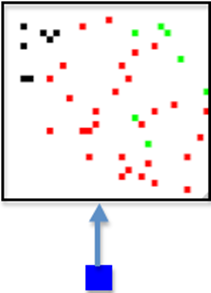
\includegraphics{img-19.png}
\end{figure}


\section{close\_display}
\label{5-Display/display:close-display}
If X display is enabled, then Rank 0 destroys the X Window and closes the display


\section{throttle}
\label{5-Display/display:throttle}
In order for better display, we wait between frames of animation.


\chapter{Core Functions}
\label{6-Core/core::doc}\label{6-Core/core:core-functions}

\section{move()}
\label{6-Core/core:move}
For of the each process's people, this function moves them around randomly.

For everyone handled by this process,

\begin{Verbatim}[commandchars=\\\{\}]
    \PYG{k}{for}\PYG{p}{(}\PYG{n}{my\PYGZus{}current\PYGZus{}person\PYGZus{}id} \PYG{o}{=} \PYG{l+m+mi}{0}\PYG{p}{;} \PYG{n}{my\PYGZus{}current\PYGZus{}person\PYGZus{}id} 
        \PYG{o}{\PYGZlt{}}\PYG{o}{=} \PYG{n}{our}\PYG{o}{-}\PYG{o}{\PYGZgt{}}\PYG{n}{our\PYGZus{}number\PYGZus{}of\PYGZus{}people} \PYG{o}{-} \PYG{l+m+mi}{1}\PYG{p}{;} \PYG{n}{my\PYGZus{}current\PYGZus{}person\PYGZus{}id}\PYG{o}{+}\PYG{o}{+}\PYG{p}{)}
\end{Verbatim}

If the person is not dead, then

\begin{Verbatim}[commandchars=\\\{\}]
        \PYG{k}{if}\PYG{p}{(}\PYG{n}{our\PYGZus{}states}\PYG{p}{[}\PYG{n}{my\PYGZus{}current\PYGZus{}person\PYGZus{}id}\PYG{p}{]} \PYG{o}{!}\PYG{o}{=} \PYG{n}{DEAD}\PYG{p}{)}
\end{Verbatim}

First, The thread randomly picks whether the person moves left or right or does not move in the x dimension.

The code uses (random() \% 3) - 1; to achieve this. (random() \% 3) returns either 0, 1, or 2. Subtracting 1 from this produces -1, 0, or 1. This means the person can move to the right, stay in place (0), or move to the left (-1).

\begin{Verbatim}[commandchars=\\\{\}]
            \PYG{c+c1}{// The thread randomly picks whether the person moves left }
            \PYG{c+c1}{// or right or does not move in the x dimension}
            \PYG{n}{my\PYGZus{}x\PYGZus{}move\PYGZus{}direction} \PYG{o}{=} \PYG{p}{(}\PYG{n}{random}\PYG{p}{(}\PYG{p}{)} \PYG{o}{\PYGZpc{}} \PYG{l+m+mi}{3}\PYG{p}{)} \PYG{o}{-} \PYG{l+m+mi}{1}\PYG{p}{;}
\end{Verbatim}

The thread then randomly picks whether the person moves up or down or does not move in the y dimension. This is similar to movement in x dimension.

\begin{Verbatim}[commandchars=\\\{\}]
            \PYG{c+c1}{// The thread randomly picks whether the person moves up}
            \PYG{c+c1}{// or down or does not move in the y dimension}
            \PYG{n}{my\PYGZus{}y\PYGZus{}move\PYGZus{}direction} \PYG{o}{=} \PYG{p}{(}\PYG{n}{random}\PYG{p}{(}\PYG{p}{)} \PYG{o}{\PYGZpc{}} \PYG{l+m+mi}{3}\PYG{p}{)} \PYG{o}{-} \PYG{l+m+mi}{1}\PYG{p}{;}
\end{Verbatim}

Next, we need to make sure that the person will remain in the bounds of the environment after moving. We check this by making sure the person’s x location is greater than or equal to 0 and less than the width of the environment and that the person’s y location is greater than or equal to 0 and less than the height of the environment. In the code, it looks like this:

\begin{Verbatim}[commandchars=\\\{\}]
            \PYG{k}{if}\PYG{p}{(} \PYG{p}{(}\PYG{n}{our\PYGZus{}x\PYGZus{}locations}\PYG{p}{[}\PYG{n}{my\PYGZus{}current\PYGZus{}person\PYGZus{}id}\PYG{p}{]} 
                    \PYG{o}{+} \PYG{n}{my\PYGZus{}x\PYGZus{}move\PYGZus{}direction} \PYG{o}{\PYGZgt{}}\PYG{o}{=} \PYG{l+m+mi}{0}\PYG{p}{)} \PYG{o}{\PYGZam{}}\PYG{o}{\PYGZam{}}
                \PYG{p}{(}\PYG{n}{our\PYGZus{}x\PYGZus{}locations}\PYG{p}{[}\PYG{n}{my\PYGZus{}current\PYGZus{}person\PYGZus{}id}\PYG{p}{]} 
                    \PYG{o}{+} \PYG{n}{my\PYGZus{}x\PYGZus{}move\PYGZus{}direction} \PYG{o}{\PYGZlt{}} \PYG{n}{environment\PYGZus{}width}\PYG{p}{)} \PYG{o}{\PYGZam{}}\PYG{o}{\PYGZam{}}
                \PYG{p}{(}\PYG{n}{our\PYGZus{}y\PYGZus{}locations}\PYG{p}{[}\PYG{n}{my\PYGZus{}current\PYGZus{}person\PYGZus{}id}\PYG{p}{]} 
                    \PYG{o}{+} \PYG{n}{my\PYGZus{}y\PYGZus{}move\PYGZus{}direction} \PYG{o}{\PYGZgt{}}\PYG{o}{=} \PYG{l+m+mi}{0}\PYG{p}{)} \PYG{o}{\PYGZam{}}\PYG{o}{\PYGZam{}}
                \PYG{p}{(}\PYG{n}{our\PYGZus{}y\PYGZus{}locations}\PYG{p}{[}\PYG{n}{my\PYGZus{}current\PYGZus{}person\PYGZus{}id}\PYG{p}{]} 
                    \PYG{o}{+} \PYG{n}{my\PYGZus{}y\PYGZus{}move\PYGZus{}direction} \PYG{o}{\PYGZlt{}} \PYG{n}{environment\PYGZus{}height}\PYG{p}{)} \PYG{p}{)}
\end{Verbatim}

Finally, The thread moves the person
\begin{figure}[htbp]
\centering

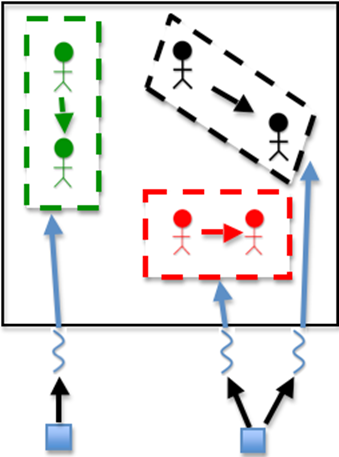
\includegraphics{img-20.png}
\end{figure}

The thread is able to achieve this by simply changing values in the
\textbf{our\_x\_locations} and \textbf{our\_y\_locations} arrays.

\begin{Verbatim}[commandchars=\\\{\}]
                \PYG{c+c1}{// The thread moves the person}
                \PYG{n}{our\PYGZus{}x\PYGZus{}locations}\PYG{p}{[}\PYG{n}{my\PYGZus{}current\PYGZus{}person\PYGZus{}id}\PYG{p}{]} \PYG{o}{+}\PYG{o}{=} \PYG{n}{my\PYGZus{}x\PYGZus{}move\PYGZus{}direction}\PYG{p}{;}
                \PYG{n}{our\PYGZus{}y\PYGZus{}locations}\PYG{p}{[}\PYG{n}{my\PYGZus{}current\PYGZus{}person\PYGZus{}id}\PYG{p}{]} \PYG{o}{+}\PYG{o}{=} \PYG{n}{my\PYGZus{}y\PYGZus{}move\PYGZus{}direction}\PYG{p}{;}
\end{Verbatim}


\section{susceptible()}
\label{6-Core/core:susceptible}
For of the each process's people, this function handles those that are ssusceptible by deciding whether or not they should be marked infected.

For everyone handled by this process,

\begin{Verbatim}[commandchars=\\\{\}]
    \PYG{k}{for}\PYG{p}{(}\PYG{n}{my\PYGZus{}current\PYGZus{}person\PYGZus{}id} \PYG{o}{=} \PYG{l+m+mi}{0}\PYG{p}{;} \PYG{n}{my\PYGZus{}current\PYGZus{}person\PYGZus{}id} 
          \PYG{o}{\PYGZlt{}}\PYG{o}{=} \PYG{n}{our}\PYG{o}{-}\PYG{o}{\PYGZgt{}}\PYG{n}{our\PYGZus{}number\PYGZus{}of\PYGZus{}people} \PYG{o}{-} \PYG{l+m+mi}{1}\PYG{p}{;} \PYG{n}{my\PYGZus{}current\PYGZus{}person\PYGZus{}id}\PYG{o}{+}\PYG{o}{+}\PYG{p}{)}
\end{Verbatim}

If the person is susceptible,

\begin{Verbatim}[commandchars=\\\{\}]
       \PYG{k}{if}\PYG{p}{(}\PYG{n}{our\PYGZus{}states}\PYG{p}{[}\PYG{n}{my\PYGZus{}current\PYGZus{}person\PYGZus{}id}\PYG{p}{]} \PYG{o}{=}\PYG{o}{=} \PYG{n}{SUSCEPTIBLE}\PYG{p}{)}
\end{Verbatim}

For each of the infected people (received earlier from all processes) or until the number of infected people nearby is 1, the thread does the following

\begin{Verbatim}[commandchars=\\\{\}]
            \PYG{k}{for}\PYG{p}{(}\PYG{n}{my\PYGZus{}person2} \PYG{o}{=} \PYG{l+m+mi}{0}\PYG{p}{;} \PYG{n}{my\PYGZus{}person2} \PYG{o}{\PYGZlt{}}\PYG{o}{=} \PYG{n}{total\PYGZus{}num\PYGZus{}infected} \PYG{o}{-} \PYG{l+m+mi}{1}
                \PYG{o}{\PYGZam{}}\PYG{o}{\PYGZam{}} \PYG{n}{my\PYGZus{}num\PYGZus{}infected\PYGZus{}nearby} \PYG{o}{\PYGZlt{}} \PYG{l+m+mi}{1}\PYG{p}{;} \PYG{n}{my\PYGZus{}person2}\PYG{o}{+}\PYG{o}{+}\PYG{p}{)}
\end{Verbatim}

If this person is within the infection radius,

\begin{Verbatim}[commandchars=\\\{\}]
                \PYG{k}{if}\PYG{p}{(}\PYG{p}{(}\PYG{n}{our\PYGZus{}x\PYGZus{}locations}\PYG{p}{[}\PYG{n}{my\PYGZus{}current\PYGZus{}person\PYGZus{}id}\PYG{p}{]} 
                    \PYG{o}{\PYGZgt{}} \PYG{n}{their\PYGZus{}infected\PYGZus{}x\PYGZus{}locations}\PYG{p}{[}\PYG{n}{my\PYGZus{}person2}\PYG{p}{]} \PYG{o}{-} \PYG{n}{infection\PYGZus{}radius}\PYG{p}{)} \PYG{o}{\PYGZam{}}\PYG{o}{\PYGZam{}}
                   \PYG{p}{(}\PYG{n}{our\PYGZus{}x\PYGZus{}locations}\PYG{p}{[}\PYG{n}{my\PYGZus{}current\PYGZus{}person\PYGZus{}id}\PYG{p}{]} 
                    \PYG{o}{\PYGZlt{}} \PYG{n}{their\PYGZus{}infected\PYGZus{}x\PYGZus{}locations}\PYG{p}{[}\PYG{n}{my\PYGZus{}person2}\PYG{p}{]} \PYG{o}{+} \PYG{n}{infection\PYGZus{}radius}\PYG{p}{)} \PYG{o}{\PYGZam{}}\PYG{o}{\PYGZam{}}
                   \PYG{p}{(}\PYG{n}{our\PYGZus{}y\PYGZus{}locations}\PYG{p}{[}\PYG{n}{my\PYGZus{}current\PYGZus{}person\PYGZus{}id}\PYG{p}{]}
                    \PYG{o}{\PYGZgt{}} \PYG{n}{their\PYGZus{}infected\PYGZus{}y\PYGZus{}locations}\PYG{p}{[}\PYG{n}{my\PYGZus{}person2}\PYG{p}{]} \PYG{o}{-} \PYG{n}{infection\PYGZus{}radius}\PYG{p}{)} \PYG{o}{\PYGZam{}}\PYG{o}{\PYGZam{}}
                   \PYG{p}{(}\PYG{n}{our\PYGZus{}y\PYGZus{}locations}\PYG{p}{[}\PYG{n}{my\PYGZus{}current\PYGZus{}person\PYGZus{}id}\PYG{p}{]}
                    \PYG{o}{\PYGZlt{}} \PYG{n}{their\PYGZus{}infected\PYGZus{}y\PYGZus{}locations}\PYG{p}{[}\PYG{n}{my\PYGZus{}person2}\PYG{p}{]} \PYG{o}{+} \PYG{n}{infection\PYGZus{}radius}\PYG{p}{)}\PYG{p}{)}
\end{Verbatim}

then, the function increments the number of infected people nearby

\begin{Verbatim}[commandchars=\\\{\}]
                    \PYG{n}{my\PYGZus{}num\PYGZus{}infected\PYGZus{}nearby}\PYG{o}{+}\PYG{o}{+}\PYG{p}{;}
\end{Verbatim}
\begin{figure}[htbp]
\centering

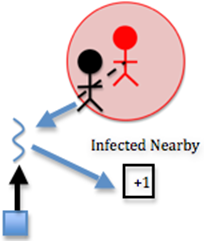
\includegraphics{img-21.png}
\end{figure}

This is where a large chunk of the algorithm’s computation occurs. Each susceptible person must be computed with each infected person to determine how many infected people are nearby each person. Two nested loops means many computations. In this step, the computation is fairly simple, however. The thread simply increments the \textbf{my\_num\_infected\_nearby} variable.

Note in the code that if the number of infected nearby is greater than or equal to 1 and we have \textbf{SHOW\_RESULTS} enabled, we increment the \textbf{our\_num\_infection\_attempts} variable. This helps us keep track of the number of attempted infections, which will help us calculate the actual contagiousness of the disease at the end of the simulation.

\begin{Verbatim}[commandchars=\\\{\}]
            \PYG{c+c1}{// The thread updates stats counter}
            \PYG{c+cp}{\PYGZsh{}}\PYG{c+cp}{ifdef SHOW\PYGZus{}RESULTS}
            \PYG{k}{if}\PYG{p}{(}\PYG{n}{my\PYGZus{}num\PYGZus{}infected\PYGZus{}nearby} \PYG{o}{\PYGZgt{}}\PYG{o}{=} \PYG{l+m+mi}{1}\PYG{p}{)}
                \PYG{n}{stats}\PYG{o}{-}\PYG{o}{\PYGZgt{}}\PYG{n}{our\PYGZus{}num\PYGZus{}infection\PYGZus{}attempts}\PYG{o}{+}\PYG{o}{+}\PYG{p}{;}
            \PYG{c+cp}{\PYGZsh{}}\PYG{c+cp}{endif}
\end{Verbatim}

If there is at least one infected person nearby, and a random number less than 100 is less than or equal to the contagiousness factor, then

\begin{Verbatim}[commandchars=\\\{\}]
            \PYG{k}{if}\PYG{p}{(}\PYG{n}{my\PYGZus{}num\PYGZus{}infected\PYGZus{}nearby} \PYG{o}{\PYGZgt{}}\PYG{o}{=} \PYG{l+m+mi}{1} \PYG{o}{\PYGZam{}}\PYG{o}{\PYGZam{}} \PYG{p}{(}\PYG{n}{random}\PYG{p}{(}\PYG{p}{)} \PYG{o}{\PYGZpc{}} \PYG{l+m+mi}{100}\PYG{p}{)} 
                \PYG{o}{\PYGZlt{}}\PYG{o}{=} \PYG{n}{contagiousness\PYGZus{}factor}\PYG{p}{)}
\end{Verbatim}

Recall that the contagiousness factor is the likelihood that the disease will be spread. We measure this as a number less than 100. For example, if there is a 30\% chance of contagiousness, we use 30 as the value of the contagiousness factor. To figure out if the disease is spread for any given interaction of people, we find a random number less than 100 and check if it is less than or equal to the contagiousness factor, because this will be equivalent to calculating the odds of actually spreading the disease (e.g. there is a 30\% chance of spreading the disease and also a 30\% chance that a random number less than 100 will be less than or equal to 30).

The thread changes this person state to infected

\begin{Verbatim}[commandchars=\\\{\}]
                \PYG{c+c1}{// The thread changes person1’s state to infected}
                \PYG{n}{our\PYGZus{}states}\PYG{p}{[}\PYG{n}{my\PYGZus{}current\PYGZus{}person\PYGZus{}id}\PYG{p}{]} \PYG{o}{=} \PYG{n}{INFECTED}\PYG{p}{;}
\end{Verbatim}

The thread updates the counters

\begin{Verbatim}[commandchars=\\\{\}]
                \PYG{c+c1}{// The thread updates the counters}
                \PYG{n}{our}\PYG{o}{-}\PYG{o}{\PYGZgt{}}\PYG{n}{our\PYGZus{}num\PYGZus{}infected}\PYG{o}{+}\PYG{o}{+}\PYG{p}{;}
                \PYG{n}{our}\PYG{o}{-}\PYG{o}{\PYGZgt{}}\PYG{n}{our\PYGZus{}num\PYGZus{}susceptible}\PYG{o}{-}\PYG{o}{-}\PYG{p}{;}
\end{Verbatim}
\begin{figure}[htbp]
\centering

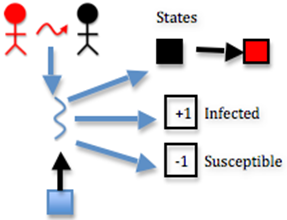
\includegraphics{img-22.png}
\end{figure}

Note in the code that if the infection succeeds and we have \textbf{SHOW\_RESULTS} enabled, we increment the \textbf{our\_num\_infections variable}. This helps us keep track of the actual number of infections, which will help us calculate the actual contagiousness of the disease at the end of the simulation.

\begin{Verbatim}[commandchars=\\\{\}]
                \PYG{c+c1}{// The thread updates stats counter}
                \PYG{c+cp}{\PYGZsh{}}\PYG{c+cp}{ifdef SHOW\PYGZus{}RESULTS}
                \PYG{n}{stats}\PYG{o}{-}\PYG{o}{\PYGZgt{}}\PYG{n}{our\PYGZus{}num\PYGZus{}infections}\PYG{o}{+}\PYG{o}{+}\PYG{p}{;}
                \PYG{c+cp}{\PYGZsh{}}\PYG{c+cp}{endif}
\end{Verbatim}


\section{infected()}
\label{6-Core/core:infected}
For of the each process's people, this function to handles those that are infected by deciding whether they should be marked immune or dead.

For everyone handled by this process,

\begin{Verbatim}[commandchars=\\\{\}]
    \PYG{k}{for}\PYG{p}{(}\PYG{n}{my\PYGZus{}current\PYGZus{}person\PYGZus{}id} \PYG{o}{=} \PYG{l+m+mi}{0}\PYG{p}{;} \PYG{n}{my\PYGZus{}current\PYGZus{}person\PYGZus{}id} 
        \PYG{o}{\PYGZlt{}}\PYG{o}{=} \PYG{n}{our}\PYG{o}{-}\PYG{o}{\PYGZgt{}}\PYG{n}{our\PYGZus{}number\PYGZus{}of\PYGZus{}people} \PYG{o}{-} \PYG{l+m+mi}{1}\PYG{p}{;} \PYG{n}{my\PYGZus{}current\PYGZus{}person\PYGZus{}id}\PYG{o}{+}\PYG{o}{+}\PYG{p}{)}
\end{Verbatim}

If the person is infected and has been for the full duration of the disease, then

\begin{Verbatim}[commandchars=\\\{\}]
        \PYG{k}{if}\PYG{p}{(}\PYG{n}{our\PYGZus{}states}\PYG{p}{[}\PYG{n}{my\PYGZus{}current\PYGZus{}person\PYGZus{}id}\PYG{p}{]} \PYG{o}{=}\PYG{o}{=} \PYG{n}{INFECTED}
            \PYG{o}{\PYGZam{}}\PYG{o}{\PYGZam{}} \PYG{n}{our\PYGZus{}num\PYGZus{}days\PYGZus{}infected}\PYG{p}{[}\PYG{n}{my\PYGZus{}current\PYGZus{}person\PYGZus{}id}\PYG{p}{]} \PYG{o}{=}\PYG{o}{=} \PYG{n}{duration\PYGZus{}of\PYGZus{}disease}\PYG{p}{)}
\end{Verbatim}

Note in the code that if we have \textbf{SHOW\_RESULTS} enabled, we increment the \textbf{our\_num\_recovery\_attempts} variable. This helps us keep track of the number of attempted recoveries, which will help us calculate the actual deadliness of the disease at the end of the simulation.

\begin{Verbatim}[commandchars=\\\{\}]
            \PYG{c+c1}{// The thread updates stats counter}
            \PYG{c+cp}{\PYGZsh{}}\PYG{c+cp}{ifdef SHOW\PYGZus{}RESULTS}
                \PYG{n}{stats}\PYG{o}{-}\PYG{o}{\PYGZgt{}}\PYG{n}{our\PYGZus{}num\PYGZus{}recovery\PYGZus{}attempts}\PYG{o}{+}\PYG{o}{+}\PYG{p}{;}
            \PYG{c+cp}{\PYGZsh{}}\PYG{c+cp}{endif}
\end{Verbatim}

If a random number less than 100 is less than the deadliness factor,

\begin{Verbatim}[commandchars=\\\{\}]
            \PYG{k}{if}\PYG{p}{(}\PYG{p}{(}\PYG{n}{random}\PYG{p}{(}\PYG{p}{)} \PYG{o}{\PYGZpc{}} \PYG{l+m+mi}{100}\PYG{p}{)} \PYG{o}{\PYGZlt{}} \PYG{n}{deadliness\PYGZus{}factor}\PYG{p}{)}
\end{Verbatim}

then, the thread changes the person’s state to dead

\begin{Verbatim}[commandchars=\\\{\}]
                \PYG{n}{our\PYGZus{}states}\PYG{p}{[}\PYG{n}{my\PYGZus{}current\PYGZus{}person\PYGZus{}id}\PYG{p}{]} \PYG{o}{=} \PYG{n}{DEAD}\PYG{p}{;}
\end{Verbatim}

and then the thread updates the counters

\begin{Verbatim}[commandchars=\\\{\}]
                \PYG{c+c1}{// The thread updates the counters}
                \PYG{n}{our}\PYG{o}{-}\PYG{o}{\PYGZgt{}}\PYG{n}{our\PYGZus{}num\PYGZus{}dead}\PYG{o}{+}\PYG{o}{+}\PYG{p}{;}
                \PYG{n}{our}\PYG{o}{-}\PYG{o}{\PYGZgt{}}\PYG{n}{our\PYGZus{}num\PYGZus{}infected}\PYG{o}{-}\PYG{o}{-}\PYG{p}{;}
\end{Verbatim}
\begin{figure}[htbp]
\centering

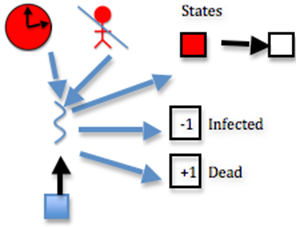
\includegraphics{img-23.png}
\end{figure}

This step is effectively the same as function susceptible, considering deadliness instead of contagiousness. The difference here is the following step:

if a random number less than 100 is less than the deadliness factor, the thread changes the person’s state to immune

\begin{Verbatim}[commandchars=\\\{\}]
                \PYG{c+c1}{// The thread changes the person’s state to immune}
                \PYG{n}{our\PYGZus{}states}\PYG{p}{[}\PYG{n}{my\PYGZus{}current\PYGZus{}person\PYGZus{}id}\PYG{p}{]} \PYG{o}{=} \PYG{n}{IMMUNE}\PYG{p}{;}
\end{Verbatim}

The thread updates the counters

\begin{Verbatim}[commandchars=\\\{\}]
                \PYG{c+c1}{// The thread updates the counters}
                \PYG{n}{our}\PYG{o}{-}\PYG{o}{\PYGZgt{}}\PYG{n}{our\PYGZus{}num\PYGZus{}immune}\PYG{o}{+}\PYG{o}{+}\PYG{p}{;}
                \PYG{n}{our}\PYG{o}{-}\PYG{o}{\PYGZgt{}}\PYG{n}{our\PYGZus{}num\PYGZus{}infected}\PYG{o}{-}\PYG{o}{-}\PYG{p}{;}
\end{Verbatim}
\begin{figure}[htbp]
\centering

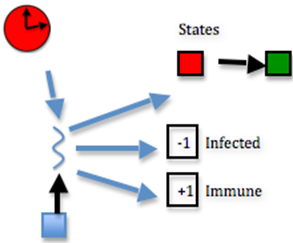
\includegraphics{img-24.png}
\end{figure}

If deadliness fails, then immunity succeeds.

Note in the code that if the person dies and we have \textbf{SHOW\_RESULTS} enabled, we increment the \textbf{our\_num\_deaths} variable. This helps us keep track of the actual number of deaths, which will help us calculate the actual deadliness of the disease at the end of the simulation.

\begin{Verbatim}[commandchars=\\\{\}]
                \PYG{c+c1}{// The thread updates stats counter}
                \PYG{c+cp}{\PYGZsh{}}\PYG{c+cp}{ifdef SHOW\PYGZus{}RESULTS}
                    \PYG{n}{stats}\PYG{o}{-}\PYG{o}{\PYGZgt{}}\PYG{n}{our\PYGZus{}num\PYGZus{}deaths}\PYG{o}{+}\PYG{o}{+}\PYG{p}{;}
                \PYG{c+cp}{\PYGZsh{}}\PYG{c+cp}{endif}
\end{Verbatim}


\section{update\_days\_infected()}
\label{6-Core/core:update-days-infected}
For of the each process's people, this function to handles those that are infected by increasing the number of days infected.

For everyone handled by this process,

\begin{Verbatim}[commandchars=\\\{\}]
    \PYG{k}{for}\PYG{p}{(}\PYG{n}{my\PYGZus{}current\PYGZus{}person\PYGZus{}id} \PYG{o}{=} \PYG{l+m+mi}{0}\PYG{p}{;} \PYG{n}{my\PYGZus{}current\PYGZus{}person\PYGZus{}id} 
        \PYG{o}{\PYGZlt{}}\PYG{o}{=} \PYG{n}{our}\PYG{o}{-}\PYG{o}{\PYGZgt{}}\PYG{n}{our\PYGZus{}number\PYGZus{}of\PYGZus{}people} \PYG{o}{-} \PYG{l+m+mi}{1}\PYG{p}{;} \PYG{n}{my\PYGZus{}current\PYGZus{}person\PYGZus{}id}\PYG{o}{+}\PYG{o}{+}\PYG{p}{)}
\end{Verbatim}

If the person is infected,

\begin{Verbatim}[commandchars=\\\{\}]
        \PYG{k}{if}\PYG{p}{(}\PYG{n}{our\PYGZus{}states}\PYG{p}{[}\PYG{n}{my\PYGZus{}current\PYGZus{}person\PYGZus{}id}\PYG{p}{]} \PYG{o}{=}\PYG{o}{=} \PYG{n}{INFECTED}\PYG{p}{)}
\end{Verbatim}

then, the function increment the number of days the person has been infected

\begin{Verbatim}[commandchars=\\\{\}]
            \PYG{n}{our\PYGZus{}num\PYGZus{}days\PYGZus{}infected}\PYG{p}{[}\PYG{n}{my\PYGZus{}current\PYGZus{}person\PYGZus{}id}\PYG{p}{]}\PYG{o}{+}\PYG{o}{+}\PYG{p}{;}
\end{Verbatim}
\begin{figure}[htbp]
\centering

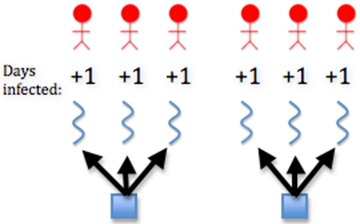
\includegraphics{img-25.png}
\end{figure}


\chapter{Finish Functions}
\label{7-Finalize/finalize:finish-functions}\label{7-Finalize/finalize::doc}

\section{show\_results()}
\label{7-Finalize/finalize:show-results}
At the end of the code, if we are choosing to show results, we print out
the final counts of susceptible, infected, immune, and dead people. We
also print the actual contagiousness and actual deadliness of the
disease. To perform these two calculations, we use the following code
(using the contagiousness as the example):

\begin{Verbatim}[commandchars=\\\{\}]
    \PYG{c+cp}{\PYGZsh{}}\PYG{c+cp}{ifdef SHOW\PYGZus{}RESULTS}
    \PYG{n}{printf}\PYG{p}{(}\PYG{l+s}{"}\PYG{l+s}{Rank \PYGZpc{}d final counts: \PYGZpc{}d susceptible, \PYGZpc{}d infected, \PYGZpc{}d immune, \PYGZpc{}d dead }\PYG{l+s+se}{\PYGZbs{}n}\PYG{l+s}{Rank \PYGZpc{}d actual contagiousness: \PYGZpc{}f }\PYG{l+s+se}{\PYGZbs{}n}\PYG{l+s}{Rank \PYGZpc{}d actual deadliness: \PYGZpc{}f }\PYG{l+s+se}{\PYGZbs{}n}\PYG{l+s}{"}\PYG{p}{,} 
        \PYG{n}{our}\PYG{o}{-}\PYG{o}{\PYGZgt{}}\PYG{n}{our\PYGZus{}rank}\PYG{p}{,} \PYG{n}{our}\PYG{o}{-}\PYG{o}{\PYGZgt{}}\PYG{n}{our\PYGZus{}num\PYGZus{}susceptible}\PYG{p}{,} \PYG{n}{our}\PYG{o}{-}\PYG{o}{\PYGZgt{}}\PYG{n}{our\PYGZus{}num\PYGZus{}infected}\PYG{p}{,} 
        \PYG{n}{our}\PYG{o}{-}\PYG{o}{\PYGZgt{}}\PYG{n}{our\PYGZus{}num\PYGZus{}immune}\PYG{p}{,} \PYG{n}{our}\PYG{o}{-}\PYG{o}{\PYGZgt{}}\PYG{n}{our\PYGZus{}num\PYGZus{}dead}\PYG{p}{,} \PYG{n}{our}\PYG{o}{-}\PYG{o}{\PYGZgt{}}\PYG{n}{our\PYGZus{}rank}\PYG{p}{,} 
        \PYG{l+m+mf}{100.0} \PYG{o}{*} \PYG{p}{(}\PYG{n}{stats}\PYG{o}{-}\PYG{o}{\PYGZgt{}}\PYG{n}{our\PYGZus{}num\PYGZus{}infections} \PYG{o}{/} \PYG{p}{(}\PYG{n}{stats}\PYG{o}{-}\PYG{o}{\PYGZgt{}}\PYG{n}{our\PYGZus{}num\PYGZus{}infection\PYGZus{}attempts} 
            \PYG{o}{=}\PYG{o}{=} \PYG{l+m+mi}{0} \PYG{o}{?} \PYG{l+m+mi}{1} \PYG{o}{:} \PYG{n}{stats}\PYG{o}{-}\PYG{o}{\PYGZgt{}}\PYG{n}{our\PYGZus{}num\PYGZus{}infection\PYGZus{}attempts}\PYG{p}{)}\PYG{p}{)}\PYG{p}{,}\PYG{n}{our}\PYG{o}{-}\PYG{o}{\PYGZgt{}}\PYG{n}{our\PYGZus{}rank}\PYG{p}{,} 
        \PYG{l+m+mf}{100.0} \PYG{o}{*} \PYG{p}{(}\PYG{n}{stats}\PYG{o}{-}\PYG{o}{\PYGZgt{}}\PYG{n}{our\PYGZus{}num\PYGZus{}deaths} \PYG{o}{/} \PYG{p}{(}\PYG{n}{stats}\PYG{o}{-}\PYG{o}{\PYGZgt{}}\PYG{n}{our\PYGZus{}num\PYGZus{}recovery\PYGZus{}attempts} 
            \PYG{o}{=}\PYG{o}{=} \PYG{l+m+mi}{0} \PYG{o}{?} \PYG{l+m+mi}{1} \PYG{o}{:} \PYG{n}{stats}\PYG{o}{-}\PYG{o}{\PYGZgt{}}\PYG{n}{our\PYGZus{}num\PYGZus{}recovery\PYGZus{}attempts}\PYG{p}{)}\PYG{p}{)}\PYG{p}{)}\PYG{p}{;}
    \PYG{c+cp}{\PYGZsh{}}\PYG{c+cp}{endif}
\end{Verbatim}

In this code, the ternary operators (? and :) are used to return one
value if something is true and another value if it isn’t. The thing we
are checking for truth is \textbf{our\_num\_infection\_attempts == 0}. If this is
true, i.e. if we didn’t attempt any infection attempts at all, then we
say there was actually 1 infection attempt (this is to avoid a divide by
zero error). Otherwise, we return the actual number of infection
attempts. This value becomes the dividend for \textbf{our\_num\_infections}; in
other words, we divide the number of actual infections by the number of
total infections. This will give us a value less than 1, so we multiply
it by 100 to obtain the actual contagiousness factor of the disease. A
similar procedure is performed to calculate the actual deadliness
factor.


\section{cleanup}
\label{7-Finalize/finalize:cleanup}
If X display is enabled, then Rank 0 destroys the X Window and closes the display

\begin{Verbatim}[commandchars=\\\{\}]
    \PYG{c+c1}{// if use X\PYGZus{}DISPLAY, do close\PYGZus{}display()}
    \PYG{c+cp}{\PYGZsh{}}\PYG{c+cp}{ifdef X\PYGZus{}DISPLAY}
    \PYG{n}{close\PYGZus{}display}\PYG{p}{(}\PYG{n}{our}\PYG{p}{,} \PYG{n}{dpy}\PYG{p}{)}\PYG{p}{;}
    \PYG{c+cp}{\PYGZsh{}}\PYG{c+cp}{endif}
\end{Verbatim}

Since we allocated our arrays dynamically, we need to release them back
to the heap using the \textbf{free} function. We do this in the reverse order
than we used \textbf{malloc}, so \textbf{environment} will come first and \textbf{x\_locations}
will come last.

\begin{Verbatim}[commandchars=\\\{\}]
    \PYG{c+c1}{// free text display environment}
    \PYG{c+cp}{\PYGZsh{}}\PYG{c+cp}{ifdef TEXT\PYGZus{}DISPLAY }
    \PYG{k+kt}{int} \PYG{n}{our\PYGZus{}current\PYGZus{}location\PYGZus{}x}\PYG{p}{;}
    \PYG{k}{for}\PYG{p}{(}\PYG{n}{our\PYGZus{}current\PYGZus{}location\PYGZus{}x} \PYG{o}{=} \PYG{n}{constant}\PYG{o}{-}\PYG{o}{\PYGZgt{}}\PYG{n}{environment\PYGZus{}width} \PYG{o}{-} \PYG{l+m+mi}{1}\PYG{p}{;} 
        \PYG{n}{our\PYGZus{}current\PYGZus{}location\PYGZus{}x} \PYG{o}{\PYGZgt{}}\PYG{o}{=} \PYG{l+m+mi}{0}\PYG{p}{;} \PYG{n}{our\PYGZus{}current\PYGZus{}location\PYGZus{}x}\PYG{o}{-}\PYG{o}{-}\PYG{p}{)}
    \PYG{p}{\PYGZob{}}
        \PYG{n}{free}\PYG{p}{(}\PYG{n}{dpy}\PYG{o}{-}\PYG{o}{\PYGZgt{}}\PYG{n}{environment}\PYG{p}{[}\PYG{n}{our\PYGZus{}current\PYGZus{}location\PYGZus{}x}\PYG{p}{]}\PYG{p}{)}\PYG{p}{;}
    \PYG{p}{\PYGZcb{}}
    \PYG{n}{free}\PYG{p}{(}\PYG{n}{dpy}\PYG{o}{-}\PYG{o}{\PYGZgt{}}\PYG{n}{environment}\PYG{p}{)}\PYG{p}{;}
    \PYG{c+cp}{\PYGZsh{}}\PYG{c+cp}{endif}

    \PYG{c+c1}{// free arrays allocated in our struct}
    \PYG{n}{free}\PYG{p}{(}\PYG{n}{our}\PYG{o}{-}\PYG{o}{\PYGZgt{}}\PYG{n}{our\PYGZus{}num\PYGZus{}days\PYGZus{}infected}\PYG{p}{)}\PYG{p}{;}
    \PYG{n}{free}\PYG{p}{(}\PYG{n}{our}\PYG{o}{-}\PYG{o}{\PYGZgt{}}\PYG{n}{our\PYGZus{}states}\PYG{p}{)}\PYG{p}{;}
    \PYG{n}{free}\PYG{p}{(}\PYG{n}{our}\PYG{o}{-}\PYG{o}{\PYGZgt{}}\PYG{n}{our\PYGZus{}infected\PYGZus{}y\PYGZus{}locations}\PYG{p}{)}\PYG{p}{;}
    \PYG{n}{free}\PYG{p}{(}\PYG{n}{our}\PYG{o}{-}\PYG{o}{\PYGZgt{}}\PYG{n}{our\PYGZus{}infected\PYGZus{}x\PYGZus{}locations}\PYG{p}{)}\PYG{p}{;}
    \PYG{n}{free}\PYG{p}{(}\PYG{n}{our}\PYG{o}{-}\PYG{o}{\PYGZgt{}}\PYG{n}{our\PYGZus{}y\PYGZus{}locations}\PYG{p}{)}\PYG{p}{;}
    \PYG{n}{free}\PYG{p}{(}\PYG{n}{our}\PYG{o}{-}\PYG{o}{\PYGZgt{}}\PYG{n}{our\PYGZus{}x\PYGZus{}locations}\PYG{p}{)}\PYG{p}{;}

    \PYG{c+c1}{// free arrays allocated in global struct}
    \PYG{n}{free}\PYG{p}{(}\PYG{n}{global}\PYG{o}{-}\PYG{o}{\PYGZgt{}}\PYG{n}{states}\PYG{p}{)}\PYG{p}{;}
    \PYG{n}{free}\PYG{p}{(}\PYG{n}{global}\PYG{o}{-}\PYG{o}{\PYGZgt{}}\PYG{n}{their\PYGZus{}infected\PYGZus{}x\PYGZus{}locations}\PYG{p}{)}\PYG{p}{;}
    \PYG{n}{free}\PYG{p}{(}\PYG{n}{global}\PYG{o}{-}\PYG{o}{\PYGZgt{}}\PYG{n}{their\PYGZus{}infected\PYGZus{}y\PYGZus{}locations}\PYG{p}{)}\PYG{p}{;}
    \PYG{n}{free}\PYG{p}{(}\PYG{n}{global}\PYG{o}{-}\PYG{o}{\PYGZgt{}}\PYG{n}{y\PYGZus{}locations}\PYG{p}{)}\PYG{p}{;}
    \PYG{n}{free}\PYG{p}{(}\PYG{n}{global}\PYG{o}{-}\PYG{o}{\PYGZgt{}}\PYG{n}{x\PYGZus{}locations}\PYG{p}{)}\PYG{p}{;}
\end{Verbatim}

Just as we initialized the MPI environment with \textbf{MPI\_Init}, we must
finalize it with \textbf{MPI\_Finalize()}. No MPI functions are allowed to occur
after \textbf{MPI\_Finalize}.

\begin{Verbatim}[commandchars=\\\{\}]
    \PYG{c+cp}{\PYGZsh{}}\PYG{c+cp}{ifdef \PYGZus{}MPI}
        \PYG{c+c1}{// MPI execution is finished; no MPI calls are allowed after this}
        \PYG{n}{MPI\PYGZus{}Finalize}\PYG{p}{(}\PYG{p}{)}\PYG{p}{;}
    \PYG{c+cp}{\PYGZsh{}}\PYG{c+cp}{endif}
\end{Verbatim}


\chapter{Build and Run the Parallel Version}
\label{7.1-BuildAndRun/mpi_build::doc}\label{7.1-BuildAndRun/mpi_build:build-and-run-the-parallel-version}
When you create the executable for this program, you will need to set some flags that are particular for your machine, particularly if you want to run it with the graphical display, which uses the X11 library.  This should work on linux machines and Mac OS X machines that have X11 installed.

Lines 13-15 in the Makefile, shown below and included with the code, are where you set paths to the X11 library and include directories.  On some linux machines you may not need to set either of these, which is why they are commented out.

In this case, lines 13 and 15 are commented because rather than seeing the display, we want to start looking at how the parallel code runs (real code wouldn't use the display for simulation modeling).  When rigging the code to test for performance, you really want to eliminate most of the output, so we have just left line 15 uncommented to see the final statistics after the whole simulation is completed.

\begin{Verbatim}[commandchars=\\\{\},numbers=left,firstnumber=1,stepnumber=1]
\PYG{c}{\PYGZsh{} DESCRIPTION:  Makefile for serial codes in C}
\PYG{c}{\PYGZsh{} AUTHOR:       Yu Zhao, Macalester College}
\PYG{c}{\PYGZsh{} DATE:         Original for Area Under A Curve module, September, 2011.}
\PYG{c}{\PYGZsh{}				Modified for Infectious Disease module, November, 2011. by Aaron Weedon}
\PYG{c}{\PYGZsh{}				Modified for Infectious Disease module, July, 2013, by Yu Zhao}

\PYG{c}{\PYGZsh{} Code prefix}
\PYG{n+nv}{PROGRAM\PYGZus{}PREFIX}\PYG{o}{=}Pandemic

\PYG{c}{\PYGZsh{} Compilers and flags}
\PYG{n+nv}{MPICC}\PYG{o}{=}mpicc

\PYG{c}{\PYGZsh{}CFLAGS+=-DTEXT\PYGZus{}DISPLAY \PYGZsh{} Uncomment to show text display}
\PYG{c}{\PYGZsh{}CFLAGS+=-DX\PYGZus{}DISPLAY -L/usr/X11R6/lib -lX11 \PYGZsh{} Uncomment to show X display}
CFLAGS+\PYG{o}{=}-DSHOW\PYGZus{}RESULTS \PYG{c}{\PYGZsh{} Uncomment to make the program print its results}

\PYG{c}{\PYGZsh{} Source files}
\PYG{n+nv}{SRCS}\PYG{o}{=}\PYG{k}{\PYGZdl{}(}PROGRAM\PYGZus{}PREFIX\PYG{k}{)}.c

\PYG{c}{\PYGZsh{} Make targets}
all: \PYG{k}{\PYGZdl{}(}PROGRAM\PYGZus{}PREFIX\PYG{k}{)}-mpi

clean: 
	rm -f \PYG{k}{\PYGZdl{}(}PROGRAM\PYGZus{}PREFIX\PYG{k}{)}-mpi

run:
	mpirun -machinefile machines -np 6 ./\PYG{k}{\PYGZdl{}(}PROGRAM\PYGZus{}PREFIX\PYG{k}{)}-mpi

\PYG{c}{\PYGZsh{} Make rules}
\PYG{k}{\PYGZdl{}(}PROGRAM\PYGZus{}PREFIX\PYG{k}{)}-mpi: \PYG{k}{\PYGZdl{}(}SRCS\PYG{k}{)}
	\PYG{k}{\PYGZdl{}(}MPICC\PYG{k}{)} -o \PYG{k}{\PYGZdl{}(}PROGRAM\PYGZus{}PREFIX\PYG{k}{)}-mpi \PYG{k}{\PYGZdl{}(}SRCS\PYG{k}{)} \PYG{k}{\PYGZdl{}(}CFLAGS\PYG{k}{)}
\end{Verbatim}


\section{Build}
\label{7.1-BuildAndRun/mpi_build:build}
\begin{Verbatim}[commandchars=\\\{\}]
\PYG{n}{make}
\end{Verbatim}


\section{Run}
\label{7.1-BuildAndRun/mpi_build:run}
\begin{Verbatim}[commandchars=\\\{\}]
mpirun -machinefile machines -np 6 ./Pandemic-mpi
\end{Verbatim}

Your instructor will provide a machines file for your cluster. You can eliminate the use of the
-machinefile machines option if you are running multiple processes on the same machine.

The default values start with a simulation of approximately 50 people.

To see what elements of the computation you can change, try this:

\begin{Verbatim}[commandchars=\\\{\}]
./Pandemic-mpi -?
\end{Verbatim}

It should give you something like this:

\begin{Verbatim}[commandchars=\\\{\}]
/Pandemic-mpi -?

Usage: ./Pandemic-mpi [-n total\_number\_of\_people][-i total\_num\_initially\_infected][-w environment\_width][-h environment\_height][-t total\_number\_of\_days][-T duration\_of\_disease][-c contagiousness\_factor][-d infection\_radius][-D deadliness\_factor][-m microseconds\_per\_day]
\end{Verbatim}

Note that these are defined and set in the \emph{parse\_args()} function in Initialize.h.

Now you can experiment running different problem sizes with different numbers of threads, like this:

\begin{Verbatim}[commandchars=\\\{\}]
mpirun -machinefile machines -np 6 ./Pandemic-mpi -n 70000 -m 0
mpirun -machinefile machines -np 8 ./Pandemic-mpi -n 70000 -m 0
\end{Verbatim}


\section{To think about}
\label{7.1-BuildAndRun/mpi_build:to-think-about}
There are preferable ways to instrument your code to time it, using the MPI function \emph{MPI\_Wtime()}.  Investigate how to use it and update this code to print running times of various sections of the code.  What loop takes the most time?

Can you calculate the speedup you get by using varying numbers of processes for a fairly large problem size?


\chapter{Including OpenMP}
\label{8-OpenMP/openmp:including-openmp}\label{8-OpenMP/openmp::doc}
\code{Download Pandemic-MPI-OMP.zip}

It is really easy to include OpenMP features into existing code we have. All we need to do is to identify all the functions that could use OpenMP. There are in total 5 functions that could use OpenMP to increase performance. The first function is the \textbf{init\_array()} function in \emph{Initialize.h} file. The next four functions are all the core functions inside \emph{Core.h} file.


\section{In Initialize.h}
\label{8-OpenMP/openmp:in-initialize-h}

\subsection{init\_array()}
\label{8-OpenMP/openmp:init-array}
This function can be divided into four parts: the first part sets the states of the initially infected people and sets the count of infected people. The second part sets states of the rest of the people and sets the of susceptible people. The third part sets random x and y locations for each people. The last part initilize the number of days infected of each people to 0.

Normally, to include OpenMP, all we need is to put \textbf{\#pragma omp parallel} in front of each of the for loops. However, our case is a little tricky. The problem is that we are reducing the counter \textbf{our\_num\_infected}. Different from most parallel structure, reduction in OpenMP is pretty easy to implement. We just need to add a reduction literal,

\begin{Verbatim}[commandchars=\\\{\}]
        \PYG{n}{reduction}\PYG{p}{(}\PYG{o}{+}\PYG{o}{:}\PYG{n}{our\PYGZus{}num\PYGZus{}infected\PYGZus{}local}\PYG{p}{)}
\end{Verbatim}

The problem lies on that the counter we are reducing is inside a structure, namely, the our structure. OpenMP does not support reduction to structures. Therefore, we solve this problem by first create local instance such as \textbf{our\_num\_infected\_local} that equals to counter \textbf{our\_num\_infected} in our struct.

\begin{Verbatim}[commandchars=\\\{\}]
    \PYG{k+kt}{int} \PYG{n}{our\PYGZus{}num\PYGZus{}infected\PYGZus{}local} \PYG{o}{=} \PYG{n}{our}\PYG{o}{-}\PYG{o}{\PYGZgt{}}\PYG{n}{our\PYGZus{}num\PYGZus{}infected}\PYG{p}{;}
\end{Verbatim}

we can then, reduce to local instance,

\begin{Verbatim}[commandchars=\\\{\}]
        \PYG{n}{our\PYGZus{}num\PYGZus{}infected\PYGZus{}local}\PYG{o}{+}\PYG{o}{+}\PYG{p}{;}
\end{Verbatim}

Finally, we put local instance back to struct.

\begin{Verbatim}[commandchars=\\\{\}]
    \PYG{n}{our}\PYG{o}{-}\PYG{o}{\PYGZgt{}}\PYG{n}{our\PYGZus{}num\PYGZus{}infected} \PYG{o}{=} \PYG{n}{our\PYGZus{}num\PYGZus{}infected\PYGZus{}local}\PYG{p}{;}
\end{Verbatim}

We then use the same reduction method for the second part of the function. The third and Fourth part of the function does not reduce any counters, which means we don't need worry about reduction at all.


\section{In Core.h}
\label{8-OpenMP/openmp:in-core-h}
There are four core functions inside \emph{Core.h} file, and all of them can be parallelized using OpenMP.


\subsection{move()}
\label{8-OpenMP/openmp:move}
This function is easy to parallelize because it does not perform any reduction. However, we need to specify the variables that is private to each OpenMP threads. \textbf{current\_person\_id} is iterator that is clearly private. \textbf{x\_move\_direction} and \textbf{y\_move\_direction} are different for every thread, which means they are private as well.

\begin{Verbatim}[commandchars=\\\{\}]
    \PYG{c+cp}{\PYGZsh{}}\PYG{c+cp}{ifdef \PYGZus{}OPENMP}
    \PYG{c+cp}{\PYGZsh{}}\PYG{c+cp}{pragma omp parallel for private(current\PYGZus{}person\PYGZus{}id, x\PYGZus{}move\PYGZus{}direction, \PYGZbs{}}
\PYG{c+cp}{        y\PYGZus{}move\PYGZus{}direction)}
    \PYG{c+cp}{\PYGZsh{}}\PYG{c+cp}{endif }
\end{Verbatim}


\subsection{susceptible()}
\label{8-OpenMP/openmp:susceptible}
This function is relatively hard to parallelize because it has four counters to reduce. Luckily, we already developed our way of reducing counters in \textbf{init\_array()} function, which means we can use same method in here.

Creating local instances

\begin{Verbatim}[commandchars=\\\{\}]
    \PYG{c+c1}{// OMP does not support reduction to struct, create local instance}
    \PYG{c+c1}{// and then put local instance back to struct}
    \PYG{k+kt}{int} \PYG{n}{num\PYGZus{}infection\PYGZus{}attempts\PYGZus{}local} \PYG{o}{=} \PYG{n}{stats}\PYG{o}{-}\PYG{o}{\PYGZgt{}}\PYG{n}{num\PYGZus{}infection\PYGZus{}attempts}\PYG{p}{;}
    \PYG{k+kt}{int} \PYG{n}{num\PYGZus{}infections\PYGZus{}local} \PYG{o}{=} \PYG{n}{stats}\PYG{o}{-}\PYG{o}{\PYGZgt{}}\PYG{n}{num\PYGZus{}infections}\PYG{p}{;}
    \PYG{k+kt}{int} \PYG{n}{num\PYGZus{}infected\PYGZus{}local} \PYG{o}{=} \PYG{n}{global}\PYG{o}{-}\PYG{o}{\PYGZgt{}}\PYG{n}{num\PYGZus{}infected}\PYG{p}{;}
    \PYG{k+kt}{int} \PYG{n}{num\PYGZus{}susceptible\PYGZus{}local} \PYG{o}{=} \PYG{n}{global}\PYG{o}{-}\PYG{o}{\PYGZgt{}}\PYG{n}{num\PYGZus{}susceptible}\PYG{p}{;}
\end{Verbatim}

OpenMP initialization

\begin{Verbatim}[commandchars=\\\{\}]
    \PYG{c+cp}{\PYGZsh{}}\PYG{c+cp}{ifdef \PYGZus{}OPENMP}
    \PYG{c+cp}{\PYGZsh{}}\PYG{c+cp}{pragma omp parallel for private(current\PYGZus{}person\PYGZus{}id, num\PYGZus{}infected\PYGZus{}nearby, \PYGZbs{}}
\PYG{c+cp}{        my\PYGZus{}person) reduction(+:num\PYGZus{}infection\PYGZus{}attempts\PYGZus{}local) \PYGZbs{}}
\PYG{c+cp}{        reduction(+:num\PYGZus{}infected\PYGZus{}local) reduction(+:num\PYGZus{}susceptible\PYGZus{}local) \PYGZbs{}}
\PYG{c+cp}{        reduction(+:num\PYGZus{}infections\PYGZus{}local)}
    \PYG{c+cp}{\PYGZsh{}}\PYG{c+cp}{endif }
\end{Verbatim}

Put local instances back to global struct

\begin{Verbatim}[commandchars=\\\{\}]
    \PYG{c+c1}{// update struct data with local instances}
    \PYG{n}{stats}\PYG{o}{-}\PYG{o}{\PYGZgt{}}\PYG{n}{num\PYGZus{}infection\PYGZus{}attempts} \PYG{o}{=} \PYG{n}{num\PYGZus{}infection\PYGZus{}attempts\PYGZus{}local}\PYG{p}{;}
    \PYG{n}{stats}\PYG{o}{-}\PYG{o}{\PYGZgt{}}\PYG{n}{num\PYGZus{}infections} \PYG{o}{=} \PYG{n}{num\PYGZus{}infections\PYGZus{}local}\PYG{p}{;}
    \PYG{n}{global}\PYG{o}{-}\PYG{o}{\PYGZgt{}}\PYG{n}{num\PYGZus{}infected} \PYG{o}{=} \PYG{n}{num\PYGZus{}infected\PYGZus{}local}\PYG{p}{;}
    \PYG{n}{global}\PYG{o}{-}\PYG{o}{\PYGZgt{}}\PYG{n}{num\PYGZus{}susceptible} \PYG{o}{=} \PYG{n}{num\PYGZus{}susceptible\PYGZus{}local}\PYG{p}{;}
\end{Verbatim}


\subsection{infected()}
\label{8-OpenMP/openmp:infected}
Similar to \textbf{susceptible()} function, we have five counters to reduce in this function.

Creating local instances

\begin{Verbatim}[commandchars=\\\{\}]
    \PYG{c+c1}{// OMP does not support reduction to struct, create local instance}
    \PYG{c+c1}{// and then put local instance back to struct}
    \PYG{k+kt}{int} \PYG{n}{num\PYGZus{}recovery\PYGZus{}attempts\PYGZus{}local} \PYG{o}{=} \PYG{n}{stats}\PYG{o}{-}\PYG{o}{\PYGZgt{}}\PYG{n}{num\PYGZus{}recovery\PYGZus{}attempts}\PYG{p}{;}
    \PYG{k+kt}{int} \PYG{n}{num\PYGZus{}deaths\PYGZus{}local} \PYG{o}{=} \PYG{n}{stats}\PYG{o}{-}\PYG{o}{\PYGZgt{}}\PYG{n}{num\PYGZus{}deaths}\PYG{p}{;}
    \PYG{k+kt}{int} \PYG{n}{num\PYGZus{}dead\PYGZus{}local} \PYG{o}{=} \PYG{n}{global}\PYG{o}{-}\PYG{o}{\PYGZgt{}}\PYG{n}{num\PYGZus{}dead}\PYG{p}{;}
    \PYG{k+kt}{int} \PYG{n}{num\PYGZus{}infected\PYGZus{}local} \PYG{o}{=} \PYG{n}{global}\PYG{o}{-}\PYG{o}{\PYGZgt{}}\PYG{n}{num\PYGZus{}infected}\PYG{p}{;}
    \PYG{k+kt}{int} \PYG{n}{num\PYGZus{}immune\PYGZus{}local} \PYG{o}{=} \PYG{n}{global}\PYG{o}{-}\PYG{o}{\PYGZgt{}}\PYG{n}{num\PYGZus{}immune}\PYG{p}{;}
\end{Verbatim}

OpenMP initialization

\begin{Verbatim}[commandchars=\\\{\}]
    \PYG{c+cp}{\PYGZsh{}}\PYG{c+cp}{ifdef \PYGZus{}OPENMP}
    \PYG{c+cp}{\PYGZsh{}}\PYG{c+cp}{pragma omp parallel for private(current\PYGZus{}person\PYGZus{}id) \PYGZbs{}}
\PYG{c+cp}{        reduction(+:num\PYGZus{}recovery\PYGZus{}attempts\PYGZus{}local) reduction(+:num\PYGZus{}dead\PYGZus{}local) \PYGZbs{}}
\PYG{c+cp}{        reduction(+:num\PYGZus{}infected\PYGZus{}local) reduction(+:num\PYGZus{}deaths\PYGZus{}local) \PYGZbs{}}
\PYG{c+cp}{        reduction(+:num\PYGZus{}immune\PYGZus{}local)}
    \PYG{c+cp}{\PYGZsh{}}\PYG{c+cp}{endif }
\end{Verbatim}

Put local instances back to global struct

\begin{Verbatim}[commandchars=\\\{\}]
    \PYG{c+c1}{// update struct data with local instances}
    \PYG{n}{stats}\PYG{o}{-}\PYG{o}{\PYGZgt{}}\PYG{n}{num\PYGZus{}recovery\PYGZus{}attempts} \PYG{o}{=} \PYG{n}{num\PYGZus{}recovery\PYGZus{}attempts\PYGZus{}local}\PYG{p}{;}
    \PYG{n}{stats}\PYG{o}{-}\PYG{o}{\PYGZgt{}}\PYG{n}{num\PYGZus{}deaths} \PYG{o}{=} \PYG{n}{num\PYGZus{}deaths\PYGZus{}local}\PYG{p}{;}
    \PYG{n}{global}\PYG{o}{-}\PYG{o}{\PYGZgt{}}\PYG{n}{num\PYGZus{}dead} \PYG{o}{=} \PYG{n}{num\PYGZus{}dead\PYGZus{}local}\PYG{p}{;}
    \PYG{n}{global}\PYG{o}{-}\PYG{o}{\PYGZgt{}}\PYG{n}{num\PYGZus{}infected} \PYG{o}{=} \PYG{n}{num\PYGZus{}infected\PYGZus{}local}\PYG{p}{;}
    \PYG{n}{global}\PYG{o}{-}\PYG{o}{\PYGZgt{}}\PYG{n}{num\PYGZus{}immune} \PYG{o}{=} \PYG{n}{num\PYGZus{}immune\PYGZus{}local}\PYG{p}{;}
\end{Verbatim}


\subsection{update\_days\_infected()}
\label{8-OpenMP/openmp:update-days-infected}
We don't have any reduction in this function, which means that the parallelization is relatively easy.

\begin{Verbatim}[commandchars=\\\{\}]
    \PYG{c+cp}{\PYGZsh{}}\PYG{c+cp}{ifdef \PYGZus{}OPENMP }
        \PYG{c+cp}{\PYGZsh{}}\PYG{c+cp}{pragma omp parallel for private(current\PYGZus{}person\PYGZus{}id)}
    \PYG{c+cp}{\PYGZsh{}}\PYG{c+cp}{endif}
\end{Verbatim}


\chapter{Including CUDA}
\label{9-Cuda/cuda:including-cuda}\label{9-Cuda/cuda::doc}
\code{Download Pandemic-MPI-CUDA.zip}

In this chapter, we will include CUDA functions into the pandemic program we developed. Since CUDA only takes over the program when we execute the core functions, most of the program remain unchanged. However, following changes are needed for CUDA set up and initialization.


\section{In Defaults.h}
\label{9-Cuda/cuda:in-defaults-h}
We need to include one extra structure in the Defualts.h file. This structure will include all the pointers used for GPU device memory and other necessary data, such as CUDA block size and CUDA grid size.


\subsection{cuda\_t struct}
\label{9-Cuda/cuda:cuda-t-struct}
\begin{Verbatim}[commandchars=\\\{\}]
\PYG{c+c1}{// All the data needed for CUDA operation: CUDA needs memory }
\PYG{c+c1}{// pointers and other information on CPU side. As more than}
\PYG{c+c1}{// one function (mainly used by CUDA.cu) need to use these }
\PYG{c+c1}{// data, we decided to use a struct to hold all these data.}
\PYG{k}{struct} \PYG{n}{cuda\PYGZus{}t} 
\PYG{p}{\PYGZob{}}
    \PYG{c+c1}{// correspond with their\PYGZus{}infected\PYGZus{}locations in global struct}
    \PYG{k+kt}{int} \PYG{o}{*}\PYG{n}{their\PYGZus{}infected\PYGZus{}x\PYGZus{}locations\PYGZus{}dev}\PYG{p}{;} 
    \PYG{k+kt}{int} \PYG{o}{*}\PYG{n}{their\PYGZus{}infected\PYGZus{}y\PYGZus{}locations\PYGZus{}dev}\PYG{p}{;} 
    \PYG{c+c1}{// correspond with our\PYGZus{}infected\PYGZus{}locations in our struct}
    \PYG{k+kt}{int} \PYG{o}{*}\PYG{n}{our\PYGZus{}x\PYGZus{}locations\PYGZus{}dev}\PYG{p}{;}
    \PYG{k+kt}{int} \PYG{o}{*}\PYG{n}{our\PYGZus{}y\PYGZus{}locations\PYGZus{}dev}\PYG{p}{;}
    \PYG{c+c1}{// correspond with our\PYGZus{}states and our\PYGZus{}num\PYGZus{}days\PYGZus{}infected in our struct }
    \PYG{k+kt}{int} \PYG{o}{*}\PYG{n}{our\PYGZus{}num\PYGZus{}days\PYGZus{}infected\PYGZus{}dev}\PYG{p}{;}
    \PYG{k+kt}{char} \PYG{o}{*}\PYG{n}{our\PYGZus{}states\PYGZus{}dev}\PYG{p}{;}

    \PYG{c+c1}{// some counter variables require atomic operations }
    \PYG{c+c1}{// correspond with states counters in our struct}
    \PYG{k+kt}{int} \PYG{o}{*}\PYG{n}{our\PYGZus{}num\PYGZus{}susceptible\PYGZus{}dev}\PYG{p}{;}
    \PYG{k+kt}{int} \PYG{o}{*}\PYG{n}{our\PYGZus{}num\PYGZus{}immune\PYGZus{}dev}\PYG{p}{;}
    \PYG{k+kt}{int} \PYG{o}{*}\PYG{n}{our\PYGZus{}num\PYGZus{}dead\PYGZus{}dev}\PYG{p}{;}
    \PYG{k+kt}{int} \PYG{o}{*}\PYG{n}{our\PYGZus{}num\PYGZus{}infected\PYGZus{}dev}\PYG{p}{;}

    \PYG{c+c1}{// correspond with variables in stats struct}
    \PYG{k+kt}{int} \PYG{o}{*}\PYG{n}{our\PYGZus{}num\PYGZus{}infections\PYGZus{}dev}\PYG{p}{;}
    \PYG{k+kt}{int} \PYG{o}{*}\PYG{n}{our\PYGZus{}num\PYGZus{}infection\PYGZus{}attempts\PYGZus{}dev}\PYG{p}{;}
    \PYG{k+kt}{int} \PYG{o}{*}\PYG{n}{our\PYGZus{}num\PYGZus{}deaths\PYGZus{}dev}\PYG{p}{;}
    \PYG{k+kt}{int} \PYG{o}{*}\PYG{n}{our\PYGZus{}num\PYGZus{}recovery\PYGZus{}attempts\PYGZus{}dev}\PYG{p}{;}

    \PYG{c+c1}{// the following four variables serve as the intermediate }
    \PYG{c+c1}{// variables. we initialized variables in stats struct as }
    \PYG{c+c1}{// doubles, but cuda atomic operations works better for }
    \PYG{c+c1}{// int. So we cast doubles to int and then cast them back }
    \PYG{k+kt}{int} \PYG{n}{our\PYGZus{}num\PYGZus{}infections\PYGZus{}int}\PYG{p}{;}
    \PYG{k+kt}{int} \PYG{n}{our\PYGZus{}num\PYGZus{}infection\PYGZus{}attempts\PYGZus{}int}\PYG{p}{;}
    \PYG{k+kt}{int} \PYG{n}{our\PYGZus{}num\PYGZus{}deaths\PYGZus{}int}\PYG{p}{;}
    \PYG{k+kt}{int} \PYG{n}{our\PYGZus{}num\PYGZus{}recovery\PYGZus{}attempts\PYGZus{}int}\PYG{p}{;}

    \PYG{c+c1}{// size used by cudaMalloc}
    \PYG{k+kt}{int} \PYG{n}{our\PYGZus{}size}\PYG{p}{;}
    \PYG{k+kt}{int} \PYG{n}{their\PYGZus{}size}\PYG{p}{;}
    \PYG{k+kt}{int} \PYG{n}{our\PYGZus{}states\PYGZus{}size}\PYG{p}{;}

    \PYG{c+c1}{// size used by cuda kernel calls}
    \PYG{k+kt}{int} \PYG{n}{numThread}\PYG{p}{;}
    \PYG{k+kt}{int} \PYG{n}{numBlock}\PYG{p}{;}
\PYG{p}{\PYGZcb{}}\PYG{p}{;}
\end{Verbatim}

\textbf{their\_infected\_x\_locations\_dev}

pointer, pointed to the memory location on device of array \textbf{their\_infected\_x\_locations\_dev}, a copy of \textbf{their\_infected\_x\_locations} on host memory.

\textbf{their\_infected\_y\_locations\_dev}

pointer, pointed to the memory location on device of array \textbf{their\_infected\_y\_locations\_dev}, a copy of \textbf{their\_infected\_y\_locations} on host memory.

\textbf{our\_x\_locations\_dev}

pointer, pointed to the memory location on device of array \textbf{our\_x\_locations\_dev}, a copy of \textbf{our\_x\_locations} on host memory.

\textbf{our\_y\_locations\_dev}

pointer, pointed to the memory location on device of array \textbf{our\_y\_locations\_dev}, a copy of \textbf{our\_y\_locations} on host memory.

\textbf{our\_num\_days\_infected\_dev}

pointer, pointed to the memory location on device of array \textbf{our\_num\_days\_infected\_dev}, a copy of \textbf{our\_num\_days\_infected} on host memory.

\textbf{our\_states\_dev}

pointer, pointed to the memory location on device of array \textbf{our\_states\_dev}, a copy of \textbf{our\_states} on host memory.

\textbf{our\_num\_susceptible\_dev}

pointer, pointed to the memory location on device of counter \textbf{our\_num\_susceptible\_dev}, a copy of \textbf{our\_num\_susceptible} on host memory.

\textbf{our\_num\_immune\_dev}

pointer, pointed to the memory location on device of counter \textbf{our\_num\_immune\_dev}, a copy of \textbf{our\_num\_immune} on host memory.

\textbf{our\_num\_dead\_dev}

pointer, pointed to the memory location on device of counter \textbf{our\_num\_dead\_dev}, a copy of \textbf{our\_num\_dead} on host memory.

\textbf{our\_num\_infected\_dev}

pointer, pointed to the memory location on device of counter \textbf{our\_num\_infected\_dev}, a copy of \textbf{our\_num\_infeced} on host memory.

\textbf{our\_num\_infections\_dev}

pointer, pointed to the memory location on device of counter \textbf{our\_num\_infections\_dev}, a copy of \textbf{our\_num\_infections} on host memory.

\textbf{our\_num\_infection\_attempts\_dev}

pointer, pointed to the memory location on device of counter \textbf{our\_num\_infection\_attempts\_dev}, a copy of \textbf{our\_num\_infection\_attempts} on host memory.

\textbf{our\_num\_deaths\_dev}

pointer, pointed to the memory location on device of counter \textbf{our\_num\_deaths\_dev}, a copy of \textbf{our\_num\_deaths} on host memory.

\textbf{our\_num\_recovery\_attempts\_dev}

pointer, pointed to the memory location on device of counter \textbf{our\_num\_recovery\_attempts\_dev}, a copy of \textbf{our\_num\_recovery\_attempts} on host memory.

\textbf{our\_num\_infections\_int}

int, holds temporary instance of \textbf{our\_num\_infections} when we cast it into a int.

\textbf{our\_num\_infection\_attempts\_int}

int, holds temporary instance of \textbf{our\_num\_infection\_attempts} when we cast it into a int.

\textbf{our\_num\_deaths\_int}

int, holds temporary instance of \textbf{our\_num\_deaths} when we cast it into a int.

\textbf{our\_num\_recovery\_attempts\_int}

int, holds temporary instance of \textbf{our\_num\_recovery\_attempts} when we cast it into a int.

\textbf{our\_size}

int, holds the size of any \textbf{integer} arrays inside \textbf{our\_t} struct.

\textbf{their\_size}

int, holds the size of any \textbf{integer} arrays inside \textbf{global\_t} struct.

\textbf{our\_states\_size}

int, holds the size of any \textbf{char} arrays inside \textbf{our\_t} struct.

\textbf{numThread}

int, holds the number of threads per block, or block size.

\textbf{numBlock}

int, holds the number of blocks per grid, or grid size.


\section{In Initialize.h}
\label{9-Cuda/cuda:in-initialize-h}
Since we are using CUDA, we need to initialize the CUDA runtime environment. To do this, we add another function in the \textbf{init()} function called \textbf{cuda\_init()}. Don't forget to include the \emph{cuda} structure in the function parameters.

\begin{Verbatim}[commandchars=\\\{\}]
\PYG{k+kt}{int} \PYG{n}{init} \PYG{p}{(}\PYG{k}{struct} \PYG{n}{global\PYGZus{}t} \PYG{o}{*}\PYG{n}{global}\PYG{p}{,} \PYG{k}{struct} \PYG{n}{const\PYGZus{}t} \PYG{o}{*}\PYG{n}{constant}\PYG{p}{,} \PYG{k}{struct} \PYG{n}{stats\PYGZus{}t} \PYG{o}{*}\PYG{n}{stats}\PYG{p}{,} 
    \PYG{k}{struct} \PYG{n}{display\PYGZus{}t} \PYG{o}{*}\PYG{n}{dpy}\PYG{p}{,} \PYG{k}{struct} \PYG{n}{cuda\PYGZus{}t} \PYG{o}{*}\PYG{n}{cuda}\PYG{p}{,} \PYG{k+kt}{int} \PYG{o}{*}\PYG{n}{c}\PYG{p}{,} \PYG{k+kt}{char} \PYG{o}{*}\PYG{o}{*}\PYG{o}{*}\PYG{n}{v}\PYG{p}{)} 
    \PYG{n}{cuda\PYGZus{}init}\PYG{p}{(}\PYG{n}{global}\PYG{p}{,} \PYG{n}{cuda}\PYG{p}{)}\PYG{p}{;}
\end{Verbatim}

Further, as we want to keep all the CUDA functions in one file, we put \textbf{cuda\_init()} inside CUDA.cu file. Therefore, we need to include this file before we can use any functions inside it.

\begin{Verbatim}[commandchars=\\\{\}]
\PYG{c+cp}{\PYGZsh{}}\PYG{c+cp}{include "CUDA.cu"      }\PYG{c+c1}{// for cuda\PYGZus{}init()}
\end{Verbatim}


\subsection{cuda\_init()}
\label{9-Cuda/cuda:cuda-init}
This function will setup the CUDA runtime environment.

Since we are allocating lots of arrays on the CUDA device memory, we first need to find out the size of each array. In total we need six arrays, of which \textbf{their\_infected\_x\_locations\_dev} and \textbf{their\_infected\_y\_locations\_dev} should be as long as the \textbf{total\_number\_of\_people}, and the rest four arrays should have length as \textbf{our\_number\_of\_people}. Note that of the four arrays above, \textbf{our\_states\_dev} is different from the rest because it holds char instead of int, which means we have to assign different size to it. The following line sets sizes we want.

\begin{Verbatim}[commandchars=\\\{\}]
    \PYG{c+c1}{// initialize size needed for cudamalloc operations}
    \PYG{n}{cuda}\PYG{o}{-}\PYG{o}{\PYGZgt{}}\PYG{n}{our\PYGZus{}size} \PYG{o}{=} \PYG{k}{sizeof}\PYG{p}{(}\PYG{k+kt}{int}\PYG{p}{)} \PYG{o}{*} \PYG{n}{our}\PYG{o}{-}\PYG{o}{\PYGZgt{}}\PYG{n}{our\PYGZus{}number\PYGZus{}of\PYGZus{}people}\PYG{p}{;}
    \PYG{n}{cuda}\PYG{o}{-}\PYG{o}{\PYGZgt{}}\PYG{n}{their\PYGZus{}size} \PYG{o}{=} \PYG{k}{sizeof}\PYG{p}{(}\PYG{k+kt}{int}\PYG{p}{)} \PYG{o}{*} \PYG{n}{global}\PYG{o}{-}\PYG{o}{\PYGZgt{}}\PYG{n}{total\PYGZus{}number\PYGZus{}of\PYGZus{}people}\PYG{p}{;}
    \PYG{n}{cuda}\PYG{o}{-}\PYG{o}{\PYGZgt{}}\PYG{n}{our\PYGZus{}states\PYGZus{}size} \PYG{o}{=} \PYG{k}{sizeof}\PYG{p}{(}\PYG{k+kt}{char}\PYG{p}{)} \PYG{o}{*} \PYG{n}{our}\PYG{o}{-}\PYG{o}{\PYGZgt{}}\PYG{n}{our\PYGZus{}number\PYGZus{}of\PYGZus{}people}\PYG{p}{;}
\end{Verbatim}

After setting up the sizes, we can allocate arrays on the device. Note that all the pointers are already initialized in the cuda structure.

\begin{Verbatim}[commandchars=\\\{\}]
    \PYG{c+c1}{// arrays in global and our struct}
    \PYG{n}{cudaMalloc}\PYG{p}{(}\PYG{p}{(}\PYG{k+kt}{void}\PYG{o}{*}\PYG{o}{*}\PYG{p}{)}\PYG{o}{\PYGZam{}}\PYG{n}{cuda}\PYG{o}{-}\PYG{o}{\PYGZgt{}}\PYG{n}{their\PYGZus{}infected\PYGZus{}x\PYGZus{}locations\PYGZus{}dev}\PYG{p}{,} \PYG{n}{cuda}\PYG{o}{-}\PYG{o}{\PYGZgt{}}\PYG{n}{their\PYGZus{}size}\PYG{p}{)}\PYG{p}{;}
    \PYG{n}{cudaMalloc}\PYG{p}{(}\PYG{p}{(}\PYG{k+kt}{void}\PYG{o}{*}\PYG{o}{*}\PYG{p}{)}\PYG{o}{\PYGZam{}}\PYG{n}{cuda}\PYG{o}{-}\PYG{o}{\PYGZgt{}}\PYG{n}{their\PYGZus{}infected\PYGZus{}y\PYGZus{}locations\PYGZus{}dev}\PYG{p}{,} \PYG{n}{cuda}\PYG{o}{-}\PYG{o}{\PYGZgt{}}\PYG{n}{their\PYGZus{}size}\PYG{p}{)}\PYG{p}{;}
    \PYG{n}{cudaMalloc}\PYG{p}{(}\PYG{p}{(}\PYG{k+kt}{void}\PYG{o}{*}\PYG{o}{*}\PYG{p}{)}\PYG{o}{\PYGZam{}}\PYG{n}{cuda}\PYG{o}{-}\PYG{o}{\PYGZgt{}}\PYG{n}{our\PYGZus{}x\PYGZus{}locations\PYGZus{}dev}\PYG{p}{,} \PYG{n}{cuda}\PYG{o}{-}\PYG{o}{\PYGZgt{}}\PYG{n}{our\PYGZus{}size}\PYG{p}{)}\PYG{p}{;}
    \PYG{n}{cudaMalloc}\PYG{p}{(}\PYG{p}{(}\PYG{k+kt}{void}\PYG{o}{*}\PYG{o}{*}\PYG{p}{)}\PYG{o}{\PYGZam{}}\PYG{n}{cuda}\PYG{o}{-}\PYG{o}{\PYGZgt{}}\PYG{n}{our\PYGZus{}y\PYGZus{}locations\PYGZus{}dev}\PYG{p}{,} \PYG{n}{cuda}\PYG{o}{-}\PYG{o}{\PYGZgt{}}\PYG{n}{our\PYGZus{}size}\PYG{p}{)}\PYG{p}{;}
    \PYG{n}{cudaMalloc}\PYG{p}{(}\PYG{p}{(}\PYG{k+kt}{void}\PYG{o}{*}\PYG{o}{*}\PYG{p}{)}\PYG{o}{\PYGZam{}}\PYG{n}{cuda}\PYG{o}{-}\PYG{o}{\PYGZgt{}}\PYG{n}{our\PYGZus{}states\PYGZus{}dev}\PYG{p}{,} \PYG{n}{cuda}\PYG{o}{-}\PYG{o}{\PYGZgt{}}\PYG{n}{our\PYGZus{}states\PYGZus{}size}\PYG{p}{)}\PYG{p}{;}
    \PYG{n}{cudaMalloc}\PYG{p}{(}\PYG{p}{(}\PYG{k+kt}{void}\PYG{o}{*}\PYG{o}{*}\PYG{p}{)}\PYG{o}{\PYGZam{}}\PYG{n}{cuda}\PYG{o}{-}\PYG{o}{\PYGZgt{}}\PYG{n}{our\PYGZus{}num\PYGZus{}days\PYGZus{}infected\PYGZus{}dev}\PYG{p}{,} \PYG{n}{cuda}\PYG{o}{-}\PYG{o}{\PYGZgt{}}\PYG{n}{our\PYGZus{}size}\PYG{p}{)}\PYG{p}{;}
\end{Verbatim}

Besides arrays, we also need in allocate spaces for the eight counters in our structure and stats structure.

\begin{Verbatim}[commandchars=\\\{\}]
    \PYG{c+c1}{// states counters in our struct}
    \PYG{n}{cudaMalloc}\PYG{p}{(}\PYG{p}{(}\PYG{k+kt}{void}\PYG{o}{*}\PYG{o}{*}\PYG{p}{)}\PYG{o}{\PYGZam{}}\PYG{n}{cuda}\PYG{o}{-}\PYG{o}{\PYGZgt{}}\PYG{n}{our\PYGZus{}num\PYGZus{}susceptible\PYGZus{}dev}\PYG{p}{,} \PYG{k}{sizeof}\PYG{p}{(}\PYG{k+kt}{int}\PYG{p}{)}\PYG{p}{)}\PYG{p}{;}
    \PYG{n}{cudaMalloc}\PYG{p}{(}\PYG{p}{(}\PYG{k+kt}{void}\PYG{o}{*}\PYG{o}{*}\PYG{p}{)}\PYG{o}{\PYGZam{}}\PYG{n}{cuda}\PYG{o}{-}\PYG{o}{\PYGZgt{}}\PYG{n}{our\PYGZus{}num\PYGZus{}immune\PYGZus{}dev}\PYG{p}{,} \PYG{k}{sizeof}\PYG{p}{(}\PYG{k+kt}{int}\PYG{p}{)}\PYG{p}{)}\PYG{p}{;}
    \PYG{n}{cudaMalloc}\PYG{p}{(}\PYG{p}{(}\PYG{k+kt}{void}\PYG{o}{*}\PYG{o}{*}\PYG{p}{)}\PYG{o}{\PYGZam{}}\PYG{n}{cuda}\PYG{o}{-}\PYG{o}{\PYGZgt{}}\PYG{n}{our\PYGZus{}num\PYGZus{}dead\PYGZus{}dev}\PYG{p}{,} \PYG{k}{sizeof}\PYG{p}{(}\PYG{k+kt}{int}\PYG{p}{)}\PYG{p}{)}\PYG{p}{;}
    \PYG{n}{cudaMalloc}\PYG{p}{(}\PYG{p}{(}\PYG{k+kt}{void}\PYG{o}{*}\PYG{o}{*}\PYG{p}{)}\PYG{o}{\PYGZam{}}\PYG{n}{cuda}\PYG{o}{-}\PYG{o}{\PYGZgt{}}\PYG{n}{our\PYGZus{}num\PYGZus{}infected\PYGZus{}dev}\PYG{p}{,} \PYG{k}{sizeof}\PYG{p}{(}\PYG{k+kt}{int}\PYG{p}{)}\PYG{p}{)}\PYG{p}{;}
    \PYG{c+cp}{\PYGZsh{}}\PYG{c+cp}{ifdef SHOW\PYGZus{}RESULTS}
    \PYG{c+c1}{// stats variables in stats struct}
    \PYG{n}{cudaMalloc}\PYG{p}{(}\PYG{p}{(}\PYG{k+kt}{void}\PYG{o}{*}\PYG{o}{*}\PYG{p}{)}\PYG{o}{\PYGZam{}}\PYG{n}{cuda}\PYG{o}{-}\PYG{o}{\PYGZgt{}}\PYG{n}{our\PYGZus{}num\PYGZus{}infections\PYGZus{}dev}\PYG{p}{,} \PYG{k}{sizeof}\PYG{p}{(}\PYG{k+kt}{int}\PYG{p}{)}\PYG{p}{)}\PYG{p}{;}
    \PYG{n}{cudaMalloc}\PYG{p}{(}\PYG{p}{(}\PYG{k+kt}{void}\PYG{o}{*}\PYG{o}{*}\PYG{p}{)}\PYG{o}{\PYGZam{}}\PYG{n}{cuda}\PYG{o}{-}\PYG{o}{\PYGZgt{}}\PYG{n}{our\PYGZus{}num\PYGZus{}infection\PYGZus{}attempts\PYGZus{}dev}\PYG{p}{,} \PYG{k}{sizeof}\PYG{p}{(}\PYG{k+kt}{int}\PYG{p}{)}\PYG{p}{)}\PYG{p}{;}
    \PYG{n}{cudaMalloc}\PYG{p}{(}\PYG{p}{(}\PYG{k+kt}{void}\PYG{o}{*}\PYG{o}{*}\PYG{p}{)}\PYG{o}{\PYGZam{}}\PYG{n}{cuda}\PYG{o}{-}\PYG{o}{\PYGZgt{}}\PYG{n}{our\PYGZus{}num\PYGZus{}deaths\PYGZus{}dev}\PYG{p}{,} \PYG{k}{sizeof}\PYG{p}{(}\PYG{k+kt}{int}\PYG{p}{)}\PYG{p}{)}\PYG{p}{;}
    \PYG{n}{cudaMalloc}\PYG{p}{(}\PYG{p}{(}\PYG{k+kt}{void}\PYG{o}{*}\PYG{o}{*}\PYG{p}{)}\PYG{o}{\PYGZam{}}\PYG{n}{cuda}\PYG{o}{-}\PYG{o}{\PYGZgt{}}\PYG{n}{our\PYGZus{}num\PYGZus{}recovery\PYGZus{}attempts\PYGZus{}dev}\PYG{p}{,} \PYG{k}{sizeof}\PYG{p}{(}\PYG{k+kt}{int}\PYG{p}{)}\PYG{p}{)}\PYG{p}{;}
    \PYG{c+cp}{\PYGZsh{}}\PYG{c+cp}{endif}
\end{Verbatim}

After allocating structure, we need to set up the random number generator. Since all the device code are executed on GPU device instead of on CPU, functions like \textbf{random()} will not work. Therefore, we need to use \href{http://docs.nvidia.com/cuda/curand/index.html}{NVIDIA cuRAND} library to generate all the random numbers. According to the documentation of cuRAND library, the normal sequence of operations to generate random number for CUDA device can be divided into seven steps. \textbf{cuda\_init()} function will cover three steps, \textbf{cuda\_run()} function will cover three steps, and \textbf{cuda\_finish()} function will cover the last step.
\begin{enumerate}
\item {} 
Create a new generator of the desired type with curandCreateGenerator().

\end{enumerate}

\begin{Verbatim}[commandchars=\\\{\}]
    \PYG{c+c1}{// create cuda random number generator}
    \PYG{n}{curandCreateGenerator}\PYG{p}{(}\PYG{o}{\PYGZam{}}\PYG{n}{gen}\PYG{p}{,} \PYG{n}{CURAND\PYGZus{}RNG\PYGZus{}PSEUDO\PYGZus{}DEFAULT}\PYG{p}{)}\PYG{p}{;}
\end{Verbatim}
\begin{enumerate}
\setcounter{enumi}{1}
\item {} 
Set the generator options; for example, use curandSetPseudoRandomGeneratorSeed() to set the seed.

\end{enumerate}

\begin{Verbatim}[commandchars=\\\{\}]
    \PYG{c+c1}{// get time }
    \PYG{n}{time}\PYG{p}{(}\PYG{o}{\PYGZam{}}\PYG{n}{current\PYGZus{}time}\PYG{p}{)}\PYG{p}{;}
    \PYG{c+c1}{// generate seed for the rand number generator}
    \PYG{n}{curandSetPseudoRandomGeneratorSeed}\PYG{p}{(}\PYG{n}{gen}\PYG{p}{,} \PYG{p}{(}\PYG{k+kt}{unsigned} \PYG{k+kt}{long}\PYG{p}{)}\PYG{n}{current\PYGZus{}time}\PYG{p}{)}\PYG{p}{;}
\end{Verbatim}
\begin{enumerate}
\setcounter{enumi}{2}
\item {} 
Allocate memory on the device with cudaMalloc().

\end{enumerate}

\begin{Verbatim}[commandchars=\\\{\}]
    \PYG{c+c1}{// array to hold random number}
    \PYG{n}{cudaMalloc}\PYG{p}{(}\PYG{p}{(}\PYG{k+kt}{void}\PYG{o}{*}\PYG{o}{*}\PYG{p}{)}\PYG{o}{\PYGZam{}}\PYG{n}{rand\PYGZus{}nums}\PYG{p}{,} \PYG{l+m+mi}{2} \PYG{o}{*} \PYG{n}{our}\PYG{o}{-}\PYG{o}{\PYGZgt{}}\PYG{n}{our\PYGZus{}number\PYGZus{}of\PYGZus{}people} \PYG{o}{*} \PYG{k}{sizeof}\PYG{p}{(}\PYG{k+kt}{float}\PYG{p}{)}\PYG{p}{)}\PYG{p}{;}
\end{Verbatim}

After generating random numbers, we need to set up block size and grid size for CUDA operations. Since the primary data type of our program is array, we can initialize only 1-D array for CUDA device functions.

Since the primary test machine for this module is \href{https://littlefe.net/parts-v4}{LittleFe}, which features NVIDIA ION Graphics (ION2), we set the block size to be 256 threads per block as the maximum active threads per multiprocessor on ION Graphics (Compute Capability 1.3) is 512. However, if you have GPU cards that are more advanced (Compute Capability 2.0+), you can set the block size to 512, 1024 or even 2048.

\begin{Verbatim}[commandchars=\\\{\}]
    \PYG{n}{cuda}\PYG{o}{-}\PYG{o}{\PYGZgt{}}\PYG{n}{numThread} \PYG{o}{=} \PYG{p}{(}\PYG{n}{our}\PYG{o}{-}\PYG{o}{\PYGZgt{}}\PYG{n}{our\PYGZus{}number\PYGZus{}of\PYGZus{}people} \PYG{o}{\PYGZlt{}} \PYG{l+m+mi}{256} \PYG{o}{?} \PYG{n}{our}\PYG{o}{-}\PYG{o}{\PYGZgt{}}\PYG{n}{our\PYGZus{}number\PYGZus{}of\PYGZus{}people} \PYG{o}{:} \PYG{l+m+mi}{256}\PYG{p}{)}\PYG{p}{;}
\end{Verbatim}

Further, if we have less than 256 people in our simulation, we initialize exactly number of people many of threads.

As for grid size, we decide grid size according to our simulation size. For example, if you have 1000 people in your simulation, program will initialize 4 blocks.

\begin{Verbatim}[commandchars=\\\{\}]
    \PYG{n}{cuda}\PYG{o}{-}\PYG{o}{\PYGZgt{}}\PYG{n}{numBlock} \PYG{o}{=} \PYG{p}{(}\PYG{n}{our}\PYG{o}{-}\PYG{o}{\PYGZgt{}}\PYG{n}{our\PYGZus{}number\PYGZus{}of\PYGZus{}people}\PYG{o}{+}\PYG{n}{cuda}\PYG{o}{-}\PYG{o}{\PYGZgt{}}\PYG{n}{numThread}\PYG{o}{-}\PYG{l+m+mi}{1}\PYG{p}{)}\PYG{o}{/}\PYG{n}{cuda}\PYG{o}{-}\PYG{o}{\PYGZgt{}}\PYG{n}{numThread}\PYG{p}{;}
\end{Verbatim}


\section{Replace file Core.h with file CUDA.cu}
\label{9-Cuda/cuda:replace-file-core-h-with-file-cuda-cu}

\subsection{CUDA Global Variable}
\label{9-Cuda/cuda:cuda-global-variable}
At any time, use of global variables outside of \textbf{main()} function is discouraged in C programming, mainly because it is really difficult to handle the scope of the program. However, as we are building a CUDA and MPI hybrid, \textbf{all} CUDA code need to be compiled with \textbf{nvcc} compiler, which means we need to separate CUDA code from other code. Normally, we should declare these variables inside cuda\_t structure we initialized in \textbf{main()} function, but the problem is that MPI compiler \textbf{mpicc} or C compiler \textbf{gcc} or \textbf{icc} does not recognize the type curandGenerator\_t, which forces us to declare global variable inside this file, which will eventually compiled by \textbf{nvcc}.

\textbf{gen}

curandGenerator\_t, which is effectively a random generator on CUDA device. A generator in CURAND encapsulates all the internal state necessary to produce a sequence of pseudorandom or quasirandom numbers.

\textbf{current\_time}

time\_t, variable we use to hold the current time. We will use this as seed.

\textbf{rand\_nums}

array, this is a pointer pointed to an array of random float numbers.


\subsection{CUDA Device Functions}
\label{9-Cuda/cuda:cuda-device-functions}
Inside Core.h file, we have four core functions for our pandemic simulation. \textbf{move()}, \textbf{susceptible()}, \textbf{infected()} and \textbf{update\_days\_infected}. Inside CUDA.cu file, we implemented those four functions with CUDA architecture.


\subsection{cuda\_move()}
\label{9-Cuda/cuda:cuda-move}
This is a CUDA implementation of the \textbf{move()} function in core functions chapter.

First, each thread randomly picks whether the person moves left or right or does not move in the x dimension.

\begin{Verbatim}[commandchars=\\\{\}]
        \PYG{c+c1}{// The thread randomly picks whether the person moves left}
        \PYG{c+c1}{// or right or does not move in the x dimension}
        \PYG{k+kt}{int} \PYG{n}{x\PYGZus{}move\PYGZus{}direction} \PYG{o}{=} \PYG{p}{(}\PYG{k+kt}{int}\PYG{p}{)}\PYG{p}{(}\PYG{n}{rand\PYGZus{}nums}\PYG{p}{[}\PYG{n}{id}\PYG{p}{]}\PYG{o}{*}\PYG{l+m+mi}{3}\PYG{p}{)} \PYG{o}{-} \PYG{l+m+mi}{1}\PYG{p}{;}
\end{Verbatim}

The code uses (int)(rand\_nums{[}id{]}*3) - 1; to achieve this. rand\_num is a array of random numbers generated before. All the random numbers in this array are floats between 0 and 1. Then, rand\_nums{[}id{]}*3 will turn all the floats to numbers between 0 and 3. After this, we can cast all the floats to int, which eventually will make all the numbers as either 0, 1 or 2. Finally, we subtract 1 from this to produce -1, 0, or 1. This means the person can move to the right(1), stay in place (0), or move to the left (-1).

The thread randomly picks whether the person moves up or down or does not move in the y dimension. This is similar to movement in x dimension.

\begin{Verbatim}[commandchars=\\\{\}]
        \PYG{c+c1}{// The thread randomly picks whether the person moves up }
        \PYG{c+c1}{// or down or does not move in the y dimension}
        \PYG{k+kt}{int} \PYG{n}{y\PYGZus{}move\PYGZus{}direction} \PYG{o}{=} \PYG{p}{(}\PYG{k+kt}{int}\PYG{p}{)}\PYG{p}{(}\PYG{n}{rand\PYGZus{}nums}\PYG{p}{[}\PYG{n}{id}\PYG{o}{+}\PYG{n}{SIZE}\PYG{p}{]}\PYG{o}{*}\PYG{l+m+mi}{3}\PYG{p}{)} \PYG{o}{-} \PYG{l+m+mi}{1}\PYG{p}{;}
\end{Verbatim}

Next, we need to make sure the person remain in the bounds of the environment after moving. We check this by making sure the person’s x location is greater than or equal to 0 and less than the width of the environment and that the person’s y location is greater than or equal to 0 and less than the height of the environment. In the code, it looks like this:

\begin{Verbatim}[commandchars=\\\{\}]
        \PYG{k}{if}\PYG{p}{(} \PYG{p}{(}\PYG{n}{x\PYGZus{}locations\PYGZus{}dev}\PYG{p}{[}\PYG{n}{id}\PYG{p}{]} \PYG{o}{+} \PYG{n}{x\PYGZus{}move\PYGZus{}direction} \PYG{o}{\PYGZgt{}}\PYG{o}{=} \PYG{l+m+mi}{0}\PYG{p}{)} \PYG{o}{\PYGZam{}}\PYG{o}{\PYGZam{}} 
            \PYG{p}{(}\PYG{n}{x\PYGZus{}locations\PYGZus{}dev}\PYG{p}{[}\PYG{n}{id}\PYG{p}{]} \PYG{o}{+} \PYG{n}{x\PYGZus{}move\PYGZus{}direction} \PYG{o}{\PYGZlt{}} \PYG{n}{environment\PYGZus{}width}\PYG{p}{)} \PYG{o}{\PYGZam{}}\PYG{o}{\PYGZam{}} 
            \PYG{p}{(}\PYG{n}{y\PYGZus{}locations\PYGZus{}dev}\PYG{p}{[}\PYG{n}{id}\PYG{p}{]} \PYG{o}{+} \PYG{n}{y\PYGZus{}move\PYGZus{}direction} \PYG{o}{\PYGZgt{}}\PYG{o}{=} \PYG{l+m+mi}{0}\PYG{p}{)} \PYG{o}{\PYGZam{}}\PYG{o}{\PYGZam{}}
            \PYG{p}{(}\PYG{n}{y\PYGZus{}locations\PYGZus{}dev}\PYG{p}{[}\PYG{n}{id}\PYG{p}{]} \PYG{o}{+} \PYG{n}{y\PYGZus{}move\PYGZus{}direction} \PYG{o}{\PYGZlt{}} \PYG{n}{environment\PYGZus{}height}\PYG{p}{)} \PYG{p}{)}
\end{Verbatim}

Finally, The thread moves the person
\begin{figure}[htbp]
\centering

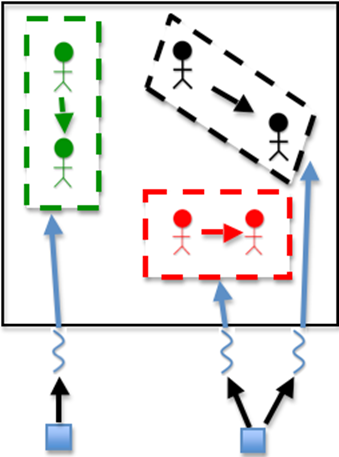
\includegraphics{img-201.png}
\end{figure}

\begin{Verbatim}[commandchars=\\\{\}]
            \PYG{c+c1}{// The thread moves the person}
            \PYG{n}{x\PYGZus{}locations\PYGZus{}dev}\PYG{p}{[}\PYG{n}{id}\PYG{p}{]} \PYG{o}{=} \PYG{n}{x\PYGZus{}locations\PYGZus{}dev}\PYG{p}{[}\PYG{n}{id}\PYG{p}{]} \PYG{o}{+} \PYG{n}{x\PYGZus{}move\PYGZus{}direction}\PYG{p}{;}
            \PYG{n}{y\PYGZus{}locations\PYGZus{}dev}\PYG{p}{[}\PYG{n}{id}\PYG{p}{]} \PYG{o}{=} \PYG{n}{y\PYGZus{}locations\PYGZus{}dev}\PYG{p}{[}\PYG{n}{id}\PYG{p}{]} \PYG{o}{+} \PYG{n}{y\PYGZus{}move\PYGZus{}direction}\PYG{p}{;}
\end{Verbatim}


\subsection{cuda\_susceptible()}
\label{9-Cuda/cuda:cuda-susceptible}
This is a CUDA implementation of the \textbf{susceptible()} function in core functions chapter.

If the person is susceptible,

\begin{Verbatim}[commandchars=\\\{\}]
    \PYG{k}{if}\PYG{p}{(}\PYG{n}{states\PYGZus{}dev}\PYG{p}{[}\PYG{n}{id}\PYG{p}{]} \PYG{o}{=}\PYG{o}{=} \PYG{n}{SUSCEPTIBLE}\PYG{p}{)}
\end{Verbatim}

For each of the infected people (received earlier from all processes) or until the number of infected people nearby is 1,

\begin{Verbatim}[commandchars=\\\{\}]
        \PYG{k}{for}\PYG{p}{(}\PYG{n}{i}\PYG{o}{=}\PYG{l+m+mi}{0}\PYG{p}{;} \PYG{n}{i}\PYG{o}{\PYGZlt{}}\PYG{o}{=}\PYG{n}{global\PYGZus{}num\PYGZus{}infected}\PYG{o}{-}\PYG{l+m+mi}{1} \PYG{o}{\PYGZam{}}\PYG{o}{\PYGZam{}} \PYG{n}{num\PYGZus{}infected\PYGZus{}nearby}\PYG{o}{\PYGZlt{}}\PYG{l+m+mi}{1}\PYG{p}{;} \PYG{n}{i}\PYG{o}{+}\PYG{o}{+}\PYG{p}{)}
\end{Verbatim}

If this person is within the infection radius,

\begin{Verbatim}[commandchars=\\\{\}]
            \PYG{k}{if}\PYG{p}{(} \PYG{p}{(}\PYG{n}{x\PYGZus{}locations\PYGZus{}dev}\PYG{p}{[}\PYG{n}{id}\PYG{p}{]} \PYG{o}{\PYGZgt{}} \PYG{n}{infected\PYGZus{}x\PYGZus{}locations\PYGZus{}dev}\PYG{p}{[}\PYG{n}{i}\PYG{p}{]} \PYG{o}{-} \PYG{n}{infection\PYGZus{}radius}\PYG{p}{)} \PYG{o}{\PYGZam{}}\PYG{o}{\PYGZam{}} 
                \PYG{p}{(}\PYG{n}{x\PYGZus{}locations\PYGZus{}dev}\PYG{p}{[}\PYG{n}{id}\PYG{p}{]} \PYG{o}{\PYGZlt{}} \PYG{n}{infected\PYGZus{}x\PYGZus{}locations\PYGZus{}dev}\PYG{p}{[}\PYG{n}{i}\PYG{p}{]} \PYG{o}{+} \PYG{n}{infection\PYGZus{}radius}\PYG{p}{)} \PYG{o}{\PYGZam{}}\PYG{o}{\PYGZam{}} 
                \PYG{p}{(}\PYG{n}{y\PYGZus{}locations\PYGZus{}dev}\PYG{p}{[}\PYG{n}{id}\PYG{p}{]} \PYG{o}{\PYGZgt{}} \PYG{n}{infected\PYGZus{}y\PYGZus{}locations\PYGZus{}dev}\PYG{p}{[}\PYG{n}{i}\PYG{p}{]} \PYG{o}{-} \PYG{n}{infection\PYGZus{}radius}\PYG{p}{)} \PYG{o}{\PYGZam{}}\PYG{o}{\PYGZam{}}
                \PYG{p}{(}\PYG{n}{y\PYGZus{}locations\PYGZus{}dev}\PYG{p}{[}\PYG{n}{id}\PYG{p}{]} \PYG{o}{\PYGZlt{}} \PYG{n}{infected\PYGZus{}y\PYGZus{}locations\PYGZus{}dev}\PYG{p}{[}\PYG{n}{i}\PYG{p}{]} \PYG{o}{+} \PYG{n}{infection\PYGZus{}radius}\PYG{p}{)} \PYG{p}{)}
\end{Verbatim}

then, the thread increments the number of infected people nearby

\begin{Verbatim}[commandchars=\\\{\}]
                \PYG{n}{num\PYGZus{}infected\PYGZus{}nearby}\PYG{o}{+}\PYG{o}{+}\PYG{p}{;}
\end{Verbatim}
\begin{figure}[htbp]
\centering

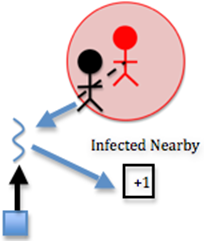
\includegraphics{img-211.png}
\end{figure}

This is where a large chunk of the algorithm’s computation occurs. Each susceptible person must be computed with each infected person to determine how many infected people are nearby each person. Two nested loops means many computations. In this step, the computation is fairly simple, however. The thread simply increments the \textbf{num\_infected\_nearby} variable.

Note in the code that if the number of infected nearby is greater than or equal to 1 and we have \textbf{SHOW\_RESULTS} enabled, we increment the \textbf{num\_infection\_attempts} variable. This helps us keep track of the number of attempted infections, which will help us calculate the actual contagiousness of the disease at the end of the simulation.

Similar to \textbf{cuda\_move()}, we also need random numbers in this function. The difference is that we need integers between -1 and 1 in \textbf{cuda\_move()} function but we need integers between 0 and 100 in this function. We obtain this random number using

\begin{Verbatim}[commandchars=\\\{\}]
        \PYG{c+c1}{// generate a random number between 0 and 100}
        \PYG{k+kt}{int} \PYG{n}{rand\PYGZus{}num} \PYG{o}{=} \PYG{p}{(}\PYG{k+kt}{int}\PYG{p}{)}\PYG{p}{(}\PYG{n}{rand\PYGZus{}nums}\PYG{p}{[}\PYG{n}{id}\PYG{p}{]}\PYG{o}{*}\PYG{l+m+mi}{100}\PYG{p}{)}\PYG{p}{;}
\end{Verbatim}

where rand\_nums is still an array of random floats between 0 and 1 and we can multiply it with 100 and cast it into a int.

If there is at least one infected person nearby, and a random number less than 100 is less than or equal to the contagiousness factor, then

\begin{Verbatim}[commandchars=\\\{\}]
        \PYG{k}{if}\PYG{p}{(}\PYG{n}{num\PYGZus{}infected\PYGZus{}nearby} \PYG{o}{\PYGZgt{}}\PYG{o}{=} \PYG{l+m+mi}{1} \PYG{o}{\PYGZam{}}\PYG{o}{\PYGZam{}} \PYG{n}{rand\PYGZus{}num} \PYG{o}{\PYGZlt{}}\PYG{o}{=} \PYG{n}{contagiousness\PYGZus{}factor}\PYG{p}{)}
\end{Verbatim}

The thread changes person’s state to infected

\begin{Verbatim}[commandchars=\\\{\}]
            \PYG{n}{states\PYGZus{}dev}\PYG{p}{[}\PYG{n}{id}\PYG{p}{]} \PYG{o}{=} \PYG{n}{INFECTED}\PYG{p}{;}
\end{Verbatim}

So far the code is similar to the \textbf{susceptible()} function executed on the CPU end. However, things get trickier from here. Since every threads need to update counters like \textbf{num\_infected} or \textbf{num\_susceptible} if someone is infected, we have racing conditions. In order to handle racing conditions and to maximize performance at the same time, we use both cuda shared memory and cuda atomic operations to update counters.

We use shared memory as temporary arrays to holds counters changed by each thread, then we would reduce this array to a single number. Finally, we use CUDA atomic operations to add the number back to actual counter.

CUDA shared memory is cache assigned to each multiprocessor. In case some of you are not familiar with the concept of multiprocessor, you can think of multiprocessor is the physical phase of blocks in CUDA coding. A typical NVIDIA GPU card with Fermi architecture (perfectly fine if you don't know what this is) supports maximum 1024 active threads per multiprocessor. This means that you can run 1024 threads concurrently on each multiprocessor. The reason we usually chose 128, 256 or 512 threads per block is that we want each multiprocessor can host exactly 8, 4 or 2 blocks on it.

However, even if we use 128 threads per block when we launch the device functions, we don't necessarily get 8 blocks per multiprocessor. Why? Because each multiprocessor has limited shared memory and registers available. GPU with Fermi architecture usually have 48KB of shared memory per multiprocessor, which means that if each block uses 8KB of shared memory, you can only initialize 6 blocks on each multiprocessor. For us, this is less of a concern because we only allocate four or five (later you will see why is four or five) arrays per block. Even we are using 1024 threads per block, we need maximum 5 * 1024 * sizeof(int) = 20KB, which is less than half of the shared memory available.

We first need to find out how many counters need atomic operations, in this function, there are four of them: \textbf{num\_infected\_dev}, \textbf{num\_susceptible\_dev}, \textbf{num\_infection\_attempts\_dev} and \textbf{num\_infections\_dev}. This is important because we need to allocate enough memory when we invoke the device function calls. Since we have four counters need atomic operations, we need to allocate four arrays, each having the length of the numbers of threads per block. The following line declares the shared memory:

\begin{Verbatim}[commandchars=\\\{\}]
\PYG{c+cm}{/* CUDA shared memory allocation */}
\PYG{k}{extern} \PYG{n}{\PYGZus{}\PYGZus{}shared\PYGZus{}\PYGZus{}} \PYG{k+kt}{int} \PYG{n}{array}\PYG{p}{[}\PYG{p}{]}\PYG{p}{;}
\end{Verbatim}

This line suggests that we allocated an array of the data type int. However, it does not specify how long the array should be. Then, inside cuda\_susceptible function, the following lines set up the four arrays we use for reduction.

\begin{Verbatim}[commandchars=\\\{\}]
    \PYG{c+c1}{// set up shared memory}
    \PYG{k+kt}{int} \PYG{o}{*}\PYG{n}{num\PYGZus{}infected} \PYG{o}{=} \PYG{p}{(}\PYG{k+kt}{int}\PYG{o}{*}\PYG{p}{)}\PYG{n}{array}\PYG{p}{;} 
    \PYG{k+kt}{int} \PYG{o}{*}\PYG{n}{num\PYGZus{}susceptible} \PYG{o}{=} \PYG{p}{(}\PYG{k+kt}{int}\PYG{o}{*}\PYG{p}{)}\PYG{o}{\PYGZam{}}\PYG{n}{num\PYGZus{}infected}\PYG{p}{[}\PYG{n}{numThread}\PYG{p}{]}\PYG{p}{;}
    \PYG{c+cp}{\PYGZsh{}}\PYG{c+cp}{ifdef SHOW\PYGZus{}RESULTS}
    \PYG{k+kt}{int} \PYG{o}{*}\PYG{n}{num\PYGZus{}infection\PYGZus{}attempts} \PYG{o}{=} \PYG{p}{(}\PYG{k+kt}{int}\PYG{o}{*}\PYG{p}{)}\PYG{o}{\PYGZam{}}\PYG{n}{num\PYGZus{}susceptible}\PYG{p}{[}\PYG{n}{numThread}\PYG{p}{]}\PYG{p}{;}
    \PYG{k+kt}{int} \PYG{o}{*}\PYG{n}{num\PYGZus{}infections} \PYG{o}{=} \PYG{p}{(}\PYG{k+kt}{int}\PYG{o}{*}\PYG{p}{)}\PYG{o}{\PYGZam{}}\PYG{n}{num\PYGZus{}infection\PYGZus{}attempts}\PYG{p}{[}\PYG{n}{numThread}\PYG{p}{]}\PYG{p}{;}
    \PYG{c+cp}{\PYGZsh{}}\PYG{c+cp}{endif}
\end{Verbatim}

we set the pointer of the first array as the pointer of the shared memory array. Then, we set the pointer of the second array as the pointer exactly \textbf{numThread} away from the pointer of the first array. We are essentially dividing the initial shared memory array into four equal sized arrays.

After shared memory setup, we need to reset the shared memory. So each thread set its corresponding shared memory elements to zero at the very beginning of the function.

\begin{Verbatim}[commandchars=\\\{\}]
    \PYG{c+c1}{// reset the shared memory}
    \PYG{n}{num\PYGZus{}infected}\PYG{p}{[}\PYG{n}{blockId}\PYG{p}{]} \PYG{o}{=} \PYG{l+m+mi}{0}\PYG{p}{;}
    \PYG{n}{num\PYGZus{}susceptible}\PYG{p}{[}\PYG{n}{blockId}\PYG{p}{]} \PYG{o}{=} \PYG{l+m+mi}{0}\PYG{p}{;}
    \PYG{c+cp}{\PYGZsh{}}\PYG{c+cp}{ifdef SHOW\PYGZus{}RESULTS}
    \PYG{n}{num\PYGZus{}infection\PYGZus{}attempts}\PYG{p}{[}\PYG{n}{blockId}\PYG{p}{]} \PYG{o}{=} \PYG{l+m+mi}{0}\PYG{p}{;}
    \PYG{n}{num\PYGZus{}infections}\PYG{p}{[}\PYG{n}{blockId}\PYG{p}{]} \PYG{o}{=} \PYG{l+m+mi}{0}\PYG{p}{;}
    \PYG{c+cp}{\PYGZsh{}}\PYG{c+cp}{endif}
\end{Verbatim}

Again this is very important. Shared memory will not clear itself after usage, and failing to clear shared memory before usage usually meaning you are starting from what ever values the shared memory is left with from last CUDA operations.

When we are updating counters, instead of adding one to or subtracting one from the actual counter located on GPU device, in this case the \textbf{num\_infected\_dev} or \textbf{num\_susceptible\_dev}counter, we add one to or subtract one from the thread's corresponding array elements.

\begin{Verbatim}[commandchars=\\\{\}]
            \PYG{c+cp}{\PYGZsh{}}\PYG{c+cp}{ifdef SHOW\PYGZus{}RESULTS}
            \PYG{n}{num\PYGZus{}infection\PYGZus{}attempts}\PYG{p}{[}\PYG{n}{blockId}\PYG{p}{]}\PYG{o}{+}\PYG{o}{+}\PYG{p}{;}
            \PYG{c+cp}{\PYGZsh{}}\PYG{c+cp}{endif}
            \PYG{n}{num\PYGZus{}infected}\PYG{p}{[}\PYG{n}{blockId}\PYG{p}{]}\PYG{o}{+}\PYG{o}{+}\PYG{p}{;}
            \PYG{n}{num\PYGZus{}susceptible}\PYG{p}{[}\PYG{n}{blockId}\PYG{p}{]}\PYG{o}{-}\PYG{o}{-}\PYG{p}{;}
            \PYG{c+cp}{\PYGZsh{}}\PYG{c+cp}{ifdef SHOW\PYGZus{}RESULTS}
            \PYG{n}{num\PYGZus{}infections}\PYG{p}{[}\PYG{n}{blockId}\PYG{p}{]}\PYG{o}{+}\PYG{o}{+}\PYG{p}{;}
            \PYG{c+cp}{\PYGZsh{}}\PYG{c+cp}{endif}
\end{Verbatim}

Finally, we need to add up the values in each array to obtain the final result. We do this using CUDA binary tree reduction. This is the official way to perform reduction operations in CUDA. The basic idea is that you create a half point on the array, use the first half thread to add the values of second half thread. This means that the array shrinks to one half of its original size. Then you can do another reduction, which will shrinks the array to one fourth of its original size. When the operation is done, the correct sum is stored at the first element of the array.The following is the implementation:

\begin{Verbatim}[commandchars=\\\{\}]
        \PYG{n}{i} \PYG{o}{=} \PYG{n}{numThread}\PYG{o}{/}\PYG{l+m+mi}{2}\PYG{p}{;}
        \PYG{k}{while} \PYG{p}{(}\PYG{n}{i} \PYG{o}{!}\PYG{o}{=} \PYG{l+m+mi}{0}\PYG{p}{)} \PYG{p}{\PYGZob{}}
            \PYG{k}{if} \PYG{p}{(}\PYG{n}{blockId} \PYG{o}{\PYGZlt{}} \PYG{n}{i}\PYG{p}{)}\PYG{p}{\PYGZob{}}
                \PYG{n}{num\PYGZus{}infected}\PYG{p}{[}\PYG{n}{blockId}\PYG{p}{]} \PYG{o}{+}\PYG{o}{=} \PYG{n}{num\PYGZus{}infected}\PYG{p}{[}\PYG{n}{blockId} \PYG{o}{+} \PYG{n}{i}\PYG{p}{]}\PYG{p}{;}
                \PYG{n}{num\PYGZus{}susceptible}\PYG{p}{[}\PYG{n}{blockId}\PYG{p}{]} \PYG{o}{+}\PYG{o}{=} \PYG{n}{num\PYGZus{}susceptible}\PYG{p}{[}\PYG{n}{blockId} \PYG{o}{+} \PYG{n}{i}\PYG{p}{]}\PYG{p}{;}
                \PYG{c+cp}{\PYGZsh{}}\PYG{c+cp}{ifdef SHOW\PYGZus{}RESULTS}
                \PYG{n}{num\PYGZus{}infection\PYGZus{}attempts}\PYG{p}{[}\PYG{n}{blockId}\PYG{p}{]} \PYG{o}{+}\PYG{o}{=} \PYG{n}{num\PYGZus{}infection\PYGZus{}attempts}\PYG{p}{[}\PYG{n}{blockId} \PYG{o}{+} \PYG{n}{i}\PYG{p}{]}\PYG{p}{;}
                \PYG{n}{num\PYGZus{}infections}\PYG{p}{[}\PYG{n}{blockId}\PYG{p}{]} \PYG{o}{+}\PYG{o}{=} \PYG{n}{num\PYGZus{}infections}\PYG{p}{[}\PYG{n}{blockId} \PYG{o}{+} \PYG{n}{i}\PYG{p}{]}\PYG{p}{;}
                \PYG{c+cp}{\PYGZsh{}}\PYG{c+cp}{endif}
            \PYG{p}{\PYGZcb{}}
            \PYG{n}{\PYGZus{}\PYGZus{}syncthreads}\PYG{p}{(}\PYG{p}{)}\PYG{p}{;}
            \PYG{n}{i} \PYG{o}{/}\PYG{o}{=} \PYG{l+m+mi}{2}\PYG{p}{;} 
        \PYG{p}{\PYGZcb{}}
\end{Verbatim}

As you probably already see, one limitation of this operation is that the array size has to be the power of 2, which essentially meaning that the block size should be power of 2 as well. If we are dealing with problem size as large as tens of thousands even millions, this won't hurt us because we are always initializing 128, 256, 512 or even 1024 threads per block. However, if we are dealing with problem size as small as 50, things gets a little bit tricker.

Therefore, we put a if statement that checks whether the size of the block is power of 2 before we do any reduction operations. Such as:

\begin{Verbatim}[commandchars=\\\{\}]
    \PYG{k}{if}\PYG{p}{(}\PYG{p}{(}\PYG{p}{(}\PYG{n}{numThread}\PYG{o}{!}\PYG{o}{=}\PYG{l+m+mi}{0}\PYG{p}{)} \PYG{o}{\PYGZam{}}\PYG{o}{\PYGZam{}} \PYG{o}{!}\PYG{p}{(}\PYG{n}{numThread} \PYG{o}{\PYGZam{}} \PYG{p}{(}\PYG{n}{numThread}\PYG{o}{-}\PYG{l+m+mi}{1}\PYG{p}{)}\PYG{p}{)}\PYG{p}{)}\PYG{p}{)}\PYG{p}{\PYGZob{}}
\end{Verbatim}

if we indeed do not have some power of 2 many of threads in a block, we can use the \textbf{first thread} of the block to add all other entries in the array to the first element.

\begin{Verbatim}[commandchars=\\\{\}]
        \PYG{k}{if}\PYG{p}{(}\PYG{n}{blockId} \PYG{o}{=}\PYG{o}{=} \PYG{l+m+mi}{0}\PYG{p}{)} \PYG{p}{\PYGZob{}}
            \PYG{k}{for}\PYG{p}{(}\PYG{n}{i}\PYG{o}{=}\PYG{l+m+mi}{1}\PYG{p}{;} \PYG{n}{i}\PYG{o}{\PYGZlt{}}\PYG{n}{numThread}\PYG{p}{;} \PYG{n}{i}\PYG{o}{+}\PYG{o}{+}\PYG{p}{)}\PYG{p}{\PYGZob{}}
                \PYG{n}{num\PYGZus{}infected}\PYG{p}{[}\PYG{l+m+mi}{0}\PYG{p}{]} \PYG{o}{+}\PYG{o}{=} \PYG{n}{num\PYGZus{}infected}\PYG{p}{[}\PYG{n}{i}\PYG{p}{]}\PYG{p}{;}
                \PYG{n}{num\PYGZus{}susceptible}\PYG{p}{[}\PYG{l+m+mi}{0}\PYG{p}{]} \PYG{o}{+}\PYG{o}{=} \PYG{n}{num\PYGZus{}susceptible}\PYG{p}{[}\PYG{n}{i}\PYG{p}{]}\PYG{p}{;}
                \PYG{c+cp}{\PYGZsh{}}\PYG{c+cp}{ifdef SHOW\PYGZus{}RESULTS}
                \PYG{n}{num\PYGZus{}infection\PYGZus{}attempts}\PYG{p}{[}\PYG{l+m+mi}{0}\PYG{p}{]} \PYG{o}{+}\PYG{o}{=} \PYG{n}{num\PYGZus{}infection\PYGZus{}attempts}\PYG{p}{[}\PYG{n}{i}\PYG{p}{]}\PYG{p}{;}
                \PYG{n}{num\PYGZus{}infections}\PYG{p}{[}\PYG{l+m+mi}{0}\PYG{p}{]} \PYG{o}{+}\PYG{o}{=} \PYG{n}{num\PYGZus{}infections}\PYG{p}{[}\PYG{n}{i}\PYG{p}{]}\PYG{p}{;}
                \PYG{c+cp}{\PYGZsh{}}\PYG{c+cp}{endif}
            \PYG{p}{\PYGZcb{}}
        \PYG{p}{\PYGZcb{}}
\end{Verbatim}

The good news is that when we run into this problem, normally means that we are dealing with a very small problem size, which should not affect the performance significantly. Notice that we could use the first thread to add up the values even if we have 128 or 256 threads per block, but the reduction takes 127 or 255 steps. However, the binary tree reduction takes 7 or 8 steps to do the same. This will make our program run much faster.

Finally, the \textbf{first thread} update the acutal counter with the first value of the array. However, we still face racing condition because more than one block could be updating the actual counter at the same time. CUDA designs functions like \textbf{atomicAdd} to handle situations like this, it can slow down your program significantly if you use \textbf{atomicAdd} too much, but since we are doing this once per block per counter, we do not suffer too much from performance loss.

\begin{Verbatim}[commandchars=\\\{\}]
    \PYG{k}{if}\PYG{p}{(}\PYG{n}{blockId} \PYG{o}{=}\PYG{o}{=} \PYG{l+m+mi}{0}\PYG{p}{)} \PYG{p}{\PYGZob{}}
        \PYG{n}{atomicAdd}\PYG{p}{(}\PYG{n}{num\PYGZus{}infected\PYGZus{}dev}\PYG{p}{,} \PYG{n}{num\PYGZus{}infected}\PYG{p}{[}\PYG{l+m+mi}{0}\PYG{p}{]}\PYG{p}{)}\PYG{p}{;}
        \PYG{n}{atomicAdd}\PYG{p}{(}\PYG{n}{num\PYGZus{}susceptible\PYGZus{}dev}\PYG{p}{,} \PYG{n}{num\PYGZus{}susceptible}\PYG{p}{[}\PYG{l+m+mi}{0}\PYG{p}{]}\PYG{p}{)}\PYG{p}{;}
        \PYG{c+cp}{\PYGZsh{}}\PYG{c+cp}{ifdef SHOW\PYGZus{}RESULTS}
        \PYG{n}{atomicAdd}\PYG{p}{(}\PYG{n}{num\PYGZus{}infection\PYGZus{}attempts\PYGZus{}dev}\PYG{p}{,} \PYG{n}{num\PYGZus{}infection\PYGZus{}attempts}\PYG{p}{[}\PYG{l+m+mi}{0}\PYG{p}{]}\PYG{p}{)}\PYG{p}{;}
        \PYG{n}{atomicAdd}\PYG{p}{(}\PYG{n}{num\PYGZus{}infections\PYGZus{}dev}\PYG{p}{,} \PYG{n}{num\PYGZus{}infections}\PYG{p}{[}\PYG{l+m+mi}{0}\PYG{p}{]}\PYG{p}{)}\PYG{p}{;}
        \PYG{c+cp}{\PYGZsh{}}\PYG{c+cp}{endif}
\end{Verbatim}
\begin{figure}[htbp]
\centering

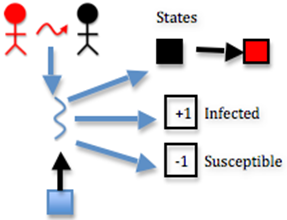
\includegraphics{img-221.png}
\end{figure}

Note in the code that if the infection succeeds and we have \textbf{SHOW\_RESULTS} enabled, we increment the \textbf{num\_infections\_dev} variable. This helps us keep track of the actual number of infections, which will help us calculate the actual contagiousness of the disease at the end of the simulation.


\subsection{cuda\_infected()}
\label{9-Cuda/cuda:cuda-infected}
This is a CUDA implementation of the \textbf{infected()} function in core functions chapter.

If the person is infected and has been for the full duration of the disease, then

\begin{Verbatim}[commandchars=\\\{\}]
    \PYG{k}{if}\PYG{p}{(}\PYG{n}{states\PYGZus{}dev}\PYG{p}{[}\PYG{n}{id}\PYG{p}{]} \PYG{o}{=}\PYG{o}{=} \PYG{n}{INFECTED} \PYG{o}{\PYGZam{}}\PYG{o}{\PYGZam{}} \PYG{n}{num\PYGZus{}days\PYGZus{}infected\PYGZus{}dev}\PYG{p}{[}\PYG{n}{id}\PYG{p}{]} \PYG{o}{=}\PYG{o}{=} \PYG{n}{duration\PYGZus{}of\PYGZus{}disease}\PYG{p}{)}
\end{Verbatim}

Note in the code that if we have \textbf{SHOW\_RESULTS} enabled, we increment the \textbf{num\_recovery\_attempts\_dev} variable. This helps us keep track of the number of attempted recoveries, which will help us calculate the actual deadliness of the disease at the end of the simulation.

\begin{Verbatim}[commandchars=\\\{\}]
        \PYG{c+cp}{\PYGZsh{}}\PYG{c+cp}{ifdef SHOW\PYGZus{}RESULTS}
        \PYG{n}{num\PYGZus{}recovery\PYGZus{}attempts}\PYG{p}{[}\PYG{n}{blockId}\PYG{p}{]}\PYG{o}{+}\PYG{o}{+}\PYG{p}{;}
        \PYG{c+cp}{\PYGZsh{}}\PYG{c+cp}{endif}
\end{Verbatim}

After this, if a random number less than 100 is less than the deadliness factor, then

\begin{Verbatim}[commandchars=\\\{\}]
        \PYG{c+c1}{// generate a random number between 0 and 100}
        \PYG{k+kt}{int} \PYG{n}{rand\PYGZus{}num} \PYG{o}{=} \PYG{p}{(}\PYG{k+kt}{int}\PYG{p}{)}\PYG{p}{(}\PYG{n}{rand\PYGZus{}nums}\PYG{p}{[}\PYG{n}{id}\PYG{p}{]}\PYG{o}{*}\PYG{l+m+mi}{100}\PYG{p}{)}\PYG{p}{;}
\end{Verbatim}

The thread changes the person’s state to dead

\begin{Verbatim}[commandchars=\\\{\}]
            \PYG{c+c1}{// The thread changes the person’s state to dead }
            \PYG{n}{states\PYGZus{}dev}\PYG{p}{[}\PYG{n}{id}\PYG{p}{]} \PYG{o}{=} \PYG{n}{DEAD}\PYG{p}{;}
\end{Verbatim}

and then the thread updates the counters

\begin{Verbatim}[commandchars=\\\{\}]
            \PYG{c+c1}{// The thread updates the counters}
            \PYG{n}{num\PYGZus{}dead}\PYG{p}{[}\PYG{n}{blockId}\PYG{p}{]}\PYG{o}{+}\PYG{o}{+}\PYG{p}{;}
            \PYG{n}{num\PYGZus{}infected}\PYG{p}{[}\PYG{n}{blockId}\PYG{p}{]}\PYG{o}{-}\PYG{o}{-}\PYG{p}{;}
            \PYG{c+cp}{\PYGZsh{}}\PYG{c+cp}{ifdef SHOW\PYGZus{}RESULTS}
            \PYG{n}{num\PYGZus{}deaths}\PYG{p}{[}\PYG{n}{blockId}\PYG{p}{]}\PYG{o}{+}\PYG{o}{+}\PYG{p}{;}
            \PYG{c+cp}{\PYGZsh{}}\PYG{c+cp}{endif}
\end{Verbatim}
\begin{figure}[htbp]
\centering

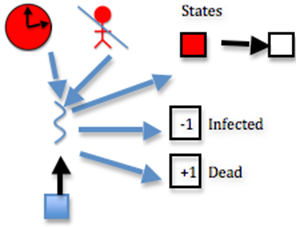
\includegraphics{img-231.png}
\end{figure}

This step is effectively the same as function susceptible, considering deadliness instead of contagiousness. The difference here is the following step:

if a random number less than 100 is less than the deadliness factor, the thread changes the person’s state to immune

\begin{Verbatim}[commandchars=\\\{\}]
            \PYG{c+c1}{// The thread changes the person’s state to immune}
            \PYG{n}{states\PYGZus{}dev}\PYG{p}{[}\PYG{n}{id}\PYG{p}{]} \PYG{o}{=} \PYG{n}{IMMUNE}\PYG{p}{;}
\end{Verbatim}

and then thread updates the counters

\begin{Verbatim}[commandchars=\\\{\}]
            \PYG{c+c1}{// The thread updates the counters}
            \PYG{n}{num\PYGZus{}immune}\PYG{p}{[}\PYG{n}{blockId}\PYG{p}{]}\PYG{o}{+}\PYG{o}{+}\PYG{p}{;}
            \PYG{n}{num\PYGZus{}infected}\PYG{p}{[}\PYG{n}{blockId}\PYG{p}{]}\PYG{o}{-}\PYG{o}{-}\PYG{p}{;}
\end{Verbatim}
\begin{figure}[htbp]
\centering

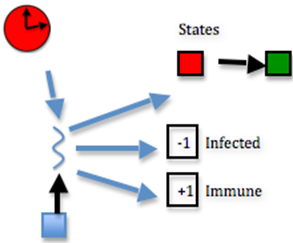
\includegraphics{img-241.png}
\end{figure}

If deadliness fails, then immunity succeeds.

Note in the code that if the person dies and we have \textbf{SHOW\_RESULTS} enabled, we increment the \textbf{num\_deaths\_dev} variable. This helps us keep track of the actual number of deaths, which will help us calculate the actual deadliness of the disease at the end of the simulation.

Note that the reduction process is the same as the \textbf{susceptible\_cuda()} function, which involves shared memory reduction and CUDA atomic operations. The only difference is that we have five counters to reduce instead of four. This will be reflected when we assign shared memory space for each block.


\subsection{cuda\_update\_days\_infected()}
\label{9-Cuda/cuda:cuda-update-days-infected}
This is the CUDA implementation of the \textbf{update\_days\_infected()} function in core functions chapter.

If the person is infected, then

\begin{Verbatim}[commandchars=\\\{\}]
    \PYG{k}{if}\PYG{p}{(}\PYG{n}{states\PYGZus{}dev}\PYG{p}{[}\PYG{n}{id}\PYG{p}{]} \PYG{o}{=}\PYG{o}{=} \PYG{n}{INFECTED}\PYG{p}{)}
\end{Verbatim}

Increment the number of days the person has been infected

\begin{Verbatim}[commandchars=\\\{\}]
        \PYG{c+c1}{// Increment the number of days the person has been infected}
        \PYG{n}{num\PYGZus{}days\PYGZus{}infected\PYGZus{}dev}\PYG{p}{[}\PYG{n}{id}\PYG{p}{]}\PYG{o}{+}\PYG{o}{+}\PYG{p}{;}
\end{Verbatim}
\begin{figure}[htbp]
\centering

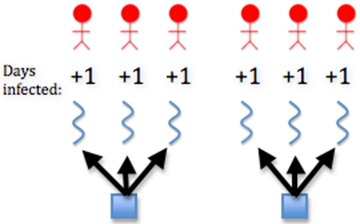
\includegraphics{img-251.png}
\end{figure}


\section{Change function calls in Pandemic.c File}
\label{9-Cuda/cuda:change-function-calls-in-pandemic-c-file}
Since we are not using core functions in Core.h file and we are using device functions on CUDA device, we need to change function calls in \textbf{main()} function.

Before changing function calls, we first need to include \emph{Cuda.cu} file before we can use any of the functions in it.

\begin{Verbatim}[commandchars=\\\{\}]
\PYG{c+cp}{\PYGZsh{}}\PYG{c+cp}{include "Infection.h"}
\PYG{c+cp}{\PYGZsh{}}\PYG{c+cp}{include "CUDA.cu"}
\PYG{c+cp}{\PYGZsh{}}\PYG{c+cp}{include "Finalize.h"}
\end{Verbatim}

Then we need to create a \emph{cuda} structure.

\begin{Verbatim}[commandchars=\\\{\}]
    \PYG{k}{struct} \PYG{n}{cuda\PYGZus{}t} \PYG{n}{cuda}\PYG{p}{;}
\end{Verbatim}

Finally, we replace the four core function calls with a single function call. Why only one function call? Because calling a CUDA function is more complicated than calling a normal function, and we want to keep all the CUDA code together in the same file. Therefore, we created a \textbf{cuda\_run()} function.


\subsection{cuda\_run()}
\label{9-Cuda/cuda:cuda-run}
This function will execute the CUDA device functions.

We first use \textbf{cudaMemcpy()} to copy data on host memory to GPU device memory. Since all of the code only performs one day's simulation, we need to put \textbf{cuda\_run()} function inside a loop. One could call all the \textbf{cudaMemcpy()} functions in each iteration, or we could divide them into two categories, those that requires constantly communicating with CPU and those who do not.

After careful examination of the code, it is not hard to find out that some functions, especially MPI functions, on host end need \textbf{infected\_x\_locations} and \textbf{infected\_y\_locations} to share infected information to all other nodes. They also need these arrays to do display. Therefore, in every iteration, we need to copy these two arrays to GPU device and copy then back to host after execution. However, other arrays or counters can reside on card from start to finish without re-copy from host to GPU device. Therefore, we implement \textbf{cudaMemcpy()} functions in the following fashion,

\begin{Verbatim}[commandchars=\\\{\}]
    \PYG{c+c1}{// copy infected locations to device in EVERY ITERATION}
    \PYG{n}{cudaMemcpy}\PYG{p}{(}\PYG{n}{cuda}\PYG{o}{-}\PYG{o}{\PYGZgt{}}\PYG{n}{their\PYGZus{}infected\PYGZus{}x\PYGZus{}locations\PYGZus{}dev}\PYG{p}{,} \PYG{n}{global}\PYG{o}{-}\PYG{o}{\PYGZgt{}}\PYG{n}{their\PYGZus{}infected\PYGZus{}x\PYGZus{}locations}\PYG{p}{,} \PYG{n}{cuda}\PYG{o}{-}\PYG{o}{\PYGZgt{}}\PYG{n}{their\PYGZus{}size}\PYG{p}{,} \PYG{n}{cudaMemcpyHostToDevice}\PYG{p}{)}\PYG{p}{;}
    \PYG{n}{cudaMemcpy}\PYG{p}{(}\PYG{n}{cuda}\PYG{o}{-}\PYG{o}{\PYGZgt{}}\PYG{n}{their\PYGZus{}infected\PYGZus{}y\PYGZus{}locations\PYGZus{}dev}\PYG{p}{,} \PYG{n}{global}\PYG{o}{-}\PYG{o}{\PYGZgt{}}\PYG{n}{their\PYGZus{}infected\PYGZus{}y\PYGZus{}locations}\PYG{p}{,} \PYG{n}{cuda}\PYG{o}{-}\PYG{o}{\PYGZgt{}}\PYG{n}{their\PYGZus{}size}\PYG{p}{,} \PYG{n}{cudaMemcpyHostToDevice}\PYG{p}{)}\PYG{p}{;}
    
    \PYG{c+c1}{// copy other information to device only in FIRST ITERATION}
    \PYG{c+c1}{// we don't need to copy these information every iteration }
    \PYG{c+c1}{// becuase they can be reused in each iteration without any}
    \PYG{c+c1}{// process at the host end.}
    \PYG{k}{if}\PYG{p}{(}\PYG{n}{our}\PYG{o}{-}\PYG{o}{\PYGZgt{}}\PYG{n}{current\PYGZus{}day} \PYG{o}{=}\PYG{o}{=} \PYG{l+m+mi}{0}\PYG{p}{)}\PYG{p}{\PYGZob{}}
        \PYG{c+c1}{// copy arrays in our struct}
        \PYG{n}{cudaMemcpy}\PYG{p}{(}\PYG{n}{cuda}\PYG{o}{-}\PYG{o}{\PYGZgt{}}\PYG{n}{our\PYGZus{}x\PYGZus{}locations\PYGZus{}dev}\PYG{p}{,} \PYG{n}{our}\PYG{o}{-}\PYG{o}{\PYGZgt{}}\PYG{n}{our\PYGZus{}x\PYGZus{}locations}\PYG{p}{,} \PYG{n}{cuda}\PYG{o}{-}\PYG{o}{\PYGZgt{}}\PYG{n}{our\PYGZus{}size}\PYG{p}{,} \PYG{n}{cudaMemcpyHostToDevice}\PYG{p}{)}\PYG{p}{;}
        \PYG{n}{cudaMemcpy}\PYG{p}{(}\PYG{n}{cuda}\PYG{o}{-}\PYG{o}{\PYGZgt{}}\PYG{n}{our\PYGZus{}y\PYGZus{}locations\PYGZus{}dev}\PYG{p}{,} \PYG{n}{our}\PYG{o}{-}\PYG{o}{\PYGZgt{}}\PYG{n}{our\PYGZus{}y\PYGZus{}locations}\PYG{p}{,} \PYG{n}{cuda}\PYG{o}{-}\PYG{o}{\PYGZgt{}}\PYG{n}{our\PYGZus{}size}\PYG{p}{,} \PYG{n}{cudaMemcpyHostToDevice}\PYG{p}{)}\PYG{p}{;}
        \PYG{n}{cudaMemcpy}\PYG{p}{(}\PYG{n}{cuda}\PYG{o}{-}\PYG{o}{\PYGZgt{}}\PYG{n}{our\PYGZus{}states\PYGZus{}dev}\PYG{p}{,} \PYG{n}{our}\PYG{o}{-}\PYG{o}{\PYGZgt{}}\PYG{n}{our\PYGZus{}states}\PYG{p}{,} \PYG{n}{cuda}\PYG{o}{-}\PYG{o}{\PYGZgt{}}\PYG{n}{our\PYGZus{}states\PYGZus{}size}\PYG{p}{,} \PYG{n}{cudaMemcpyHostToDevice}\PYG{p}{)}\PYG{p}{;}
        \PYG{n}{cudaMemcpy}\PYG{p}{(}\PYG{n}{cuda}\PYG{o}{-}\PYG{o}{\PYGZgt{}}\PYG{n}{our\PYGZus{}num\PYGZus{}days\PYGZus{}infected\PYGZus{}dev}\PYG{p}{,} \PYG{n}{our}\PYG{o}{-}\PYG{o}{\PYGZgt{}}\PYG{n}{our\PYGZus{}num\PYGZus{}days\PYGZus{}infected}\PYG{p}{,} \PYG{n}{cuda}\PYG{o}{-}\PYG{o}{\PYGZgt{}}\PYG{n}{our\PYGZus{}size}\PYG{p}{,} \PYG{n}{cudaMemcpyHostToDevice}\PYG{p}{)}\PYG{p}{;}
        \PYG{c+c1}{// copy states counters in our struct}
        \PYG{n}{cudaMemcpy}\PYG{p}{(}\PYG{n}{cuda}\PYG{o}{-}\PYG{o}{\PYGZgt{}}\PYG{n}{our\PYGZus{}num\PYGZus{}susceptible\PYGZus{}dev}\PYG{p}{,} \PYG{o}{\PYGZam{}}\PYG{n}{our}\PYG{o}{-}\PYG{o}{\PYGZgt{}}\PYG{n}{our\PYGZus{}num\PYGZus{}susceptible}\PYG{p}{,} \PYG{k}{sizeof}\PYG{p}{(}\PYG{k+kt}{int}\PYG{p}{)}\PYG{p}{,} \PYG{n}{cudaMemcpyHostToDevice}\PYG{p}{)}\PYG{p}{;}
        \PYG{n}{cudaMemcpy}\PYG{p}{(}\PYG{n}{cuda}\PYG{o}{-}\PYG{o}{\PYGZgt{}}\PYG{n}{our\PYGZus{}num\PYGZus{}immune\PYGZus{}dev}\PYG{p}{,} \PYG{o}{\PYGZam{}}\PYG{n}{our}\PYG{o}{-}\PYG{o}{\PYGZgt{}}\PYG{n}{our\PYGZus{}num\PYGZus{}immune}\PYG{p}{,} \PYG{k}{sizeof}\PYG{p}{(}\PYG{k+kt}{int}\PYG{p}{)}\PYG{p}{,} \PYG{n}{cudaMemcpyHostToDevice}\PYG{p}{)}\PYG{p}{;}
        \PYG{n}{cudaMemcpy}\PYG{p}{(}\PYG{n}{cuda}\PYG{o}{-}\PYG{o}{\PYGZgt{}}\PYG{n}{our\PYGZus{}num\PYGZus{}dead\PYGZus{}dev}\PYG{p}{,} \PYG{o}{\PYGZam{}}\PYG{n}{our}\PYG{o}{-}\PYG{o}{\PYGZgt{}}\PYG{n}{our\PYGZus{}num\PYGZus{}dead}\PYG{p}{,} \PYG{k}{sizeof}\PYG{p}{(}\PYG{k+kt}{int}\PYG{p}{)}\PYG{p}{,} \PYG{n}{cudaMemcpyHostToDevice}\PYG{p}{)}\PYG{p}{;}
        \PYG{n}{cudaMemcpy}\PYG{p}{(}\PYG{n}{cuda}\PYG{o}{-}\PYG{o}{\PYGZgt{}}\PYG{n}{our\PYGZus{}num\PYGZus{}infected\PYGZus{}dev}\PYG{p}{,} \PYG{o}{\PYGZam{}}\PYG{n}{our}\PYG{o}{-}\PYG{o}{\PYGZgt{}}\PYG{n}{our\PYGZus{}num\PYGZus{}infected}\PYG{p}{,} \PYG{k}{sizeof}\PYG{p}{(}\PYG{k+kt}{int}\PYG{p}{)}\PYG{p}{,} \PYG{n}{cudaMemcpyHostToDevice}\PYG{p}{)}\PYG{p}{;}
        
        \PYG{c+cp}{\PYGZsh{}}\PYG{c+cp}{ifdef SHOW\PYGZus{}RESULTS}
        \PYG{c+c1}{// variables in stats data are initialized as doubles, yet CUDA}
        \PYG{c+c1}{// atomic operations prefer integer than doubles. Therefore, we}
        \PYG{c+c1}{// cast doubles to integer before the cudaMemcpy operations.}
        \PYG{n}{cuda}\PYG{o}{-}\PYG{o}{\PYGZgt{}}\PYG{n}{our\PYGZus{}num\PYGZus{}infections\PYGZus{}int} \PYG{o}{=} \PYG{p}{(}\PYG{k+kt}{int}\PYG{p}{)}\PYG{n}{stats}\PYG{o}{-}\PYG{o}{\PYGZgt{}}\PYG{n}{our\PYGZus{}num\PYGZus{}infections}\PYG{p}{;}
        \PYG{n}{cuda}\PYG{o}{-}\PYG{o}{\PYGZgt{}}\PYG{n}{our\PYGZus{}num\PYGZus{}infection\PYGZus{}attempts\PYGZus{}int} \PYG{o}{=} \PYG{p}{(}\PYG{k+kt}{int}\PYG{p}{)}\PYG{n}{stats}\PYG{o}{-}\PYG{o}{\PYGZgt{}}\PYG{n}{our\PYGZus{}num\PYGZus{}infection\PYGZus{}attempts}\PYG{p}{;}
        \PYG{n}{cuda}\PYG{o}{-}\PYG{o}{\PYGZgt{}}\PYG{n}{our\PYGZus{}num\PYGZus{}deaths\PYGZus{}int} \PYG{o}{=} \PYG{p}{(}\PYG{k+kt}{int}\PYG{p}{)}\PYG{n}{stats}\PYG{o}{-}\PYG{o}{\PYGZgt{}}\PYG{n}{our\PYGZus{}num\PYGZus{}deaths}\PYG{p}{;}
        \PYG{n}{cuda}\PYG{o}{-}\PYG{o}{\PYGZgt{}}\PYG{n}{our\PYGZus{}num\PYGZus{}recovery\PYGZus{}attempts\PYGZus{}int} \PYG{o}{=} \PYG{p}{(}\PYG{k+kt}{int}\PYG{p}{)}\PYG{n}{stats}\PYG{o}{-}\PYG{o}{\PYGZgt{}}\PYG{n}{our\PYGZus{}num\PYGZus{}recovery\PYGZus{}attempts}\PYG{p}{;}
        \PYG{c+c1}{// copy stats variables in stats struct}
        \PYG{n}{cudaMemcpy}\PYG{p}{(}\PYG{n}{cuda}\PYG{o}{-}\PYG{o}{\PYGZgt{}}\PYG{n}{our\PYGZus{}num\PYGZus{}infections\PYGZus{}dev}\PYG{p}{,} \PYG{o}{\PYGZam{}}\PYG{n}{cuda}\PYG{o}{-}\PYG{o}{\PYGZgt{}}\PYG{n}{our\PYGZus{}num\PYGZus{}infections\PYGZus{}int}\PYG{p}{,} \PYG{k}{sizeof}\PYG{p}{(}\PYG{k+kt}{int}\PYG{p}{)}\PYG{p}{,} \PYG{n}{cudaMemcpyHostToDevice}\PYG{p}{)}\PYG{p}{;}
        \PYG{n}{cudaMemcpy}\PYG{p}{(}\PYG{n}{cuda}\PYG{o}{-}\PYG{o}{\PYGZgt{}}\PYG{n}{our\PYGZus{}num\PYGZus{}infection\PYGZus{}attempts\PYGZus{}dev}\PYG{p}{,} \PYG{o}{\PYGZam{}}\PYG{n}{cuda}\PYG{o}{-}\PYG{o}{\PYGZgt{}}\PYG{n}{our\PYGZus{}num\PYGZus{}infection\PYGZus{}attempts\PYGZus{}int}\PYG{p}{,} \PYG{k}{sizeof}\PYG{p}{(}\PYG{k+kt}{int}\PYG{p}{)}\PYG{p}{,} \PYG{n}{cudaMemcpyHostToDevice}\PYG{p}{)}\PYG{p}{;}
        \PYG{n}{cudaMemcpy}\PYG{p}{(}\PYG{n}{cuda}\PYG{o}{-}\PYG{o}{\PYGZgt{}}\PYG{n}{our\PYGZus{}num\PYGZus{}deaths\PYGZus{}dev}\PYG{p}{,} \PYG{o}{\PYGZam{}}\PYG{n}{cuda}\PYG{o}{-}\PYG{o}{\PYGZgt{}}\PYG{n}{our\PYGZus{}num\PYGZus{}deaths\PYGZus{}int}\PYG{p}{,} \PYG{k}{sizeof}\PYG{p}{(}\PYG{k+kt}{int}\PYG{p}{)}\PYG{p}{,} \PYG{n}{cudaMemcpyHostToDevice}\PYG{p}{)}\PYG{p}{;}
        \PYG{n}{cudaMemcpy}\PYG{p}{(}\PYG{n}{cuda}\PYG{o}{-}\PYG{o}{\PYGZgt{}}\PYG{n}{our\PYGZus{}num\PYGZus{}recovery\PYGZus{}attempts\PYGZus{}dev}\PYG{p}{,} \PYG{o}{\PYGZam{}}\PYG{n}{cuda}\PYG{o}{-}\PYG{o}{\PYGZgt{}}\PYG{n}{our\PYGZus{}num\PYGZus{}recovery\PYGZus{}attempts\PYGZus{}int}\PYG{p}{,} \PYG{k}{sizeof}\PYG{p}{(}\PYG{k+kt}{int}\PYG{p}{)}\PYG{p}{,} \PYG{n}{cudaMemcpyHostToDevice}\PYG{p}{)}\PYG{p}{;}
        \PYG{c+cp}{\PYGZsh{}}\PYG{c+cp}{endif}
    \PYG{p}{\PYGZcb{}}
\end{Verbatim}

where \textbf{if(our-\textgreater{}current\_day == 0)} makes sure that most of the data only gets copied in the first iteration, instead of in every iteration.

Another thing you probably noticed is that we cast stats counters to int before sending them to the GPU device memory.

\begin{Verbatim}[commandchars=\\\{\}]
        \PYG{n}{cuda}\PYG{o}{-}\PYG{o}{\PYGZgt{}}\PYG{n}{our\PYGZus{}num\PYGZus{}infections\PYGZus{}int} \PYG{o}{=} \PYG{p}{(}\PYG{k+kt}{int}\PYG{p}{)}\PYG{n}{stats}\PYG{o}{-}\PYG{o}{\PYGZgt{}}\PYG{n}{our\PYGZus{}num\PYGZus{}infections}\PYG{p}{;}
        \PYG{n}{cuda}\PYG{o}{-}\PYG{o}{\PYGZgt{}}\PYG{n}{our\PYGZus{}num\PYGZus{}infection\PYGZus{}attempts\PYGZus{}int} \PYG{o}{=} \PYG{p}{(}\PYG{k+kt}{int}\PYG{p}{)}\PYG{n}{stats}\PYG{o}{-}\PYG{o}{\PYGZgt{}}\PYG{n}{our\PYGZus{}num\PYGZus{}infection\PYGZus{}attempts}\PYG{p}{;}
        \PYG{n}{cuda}\PYG{o}{-}\PYG{o}{\PYGZgt{}}\PYG{n}{our\PYGZus{}num\PYGZus{}deaths\PYGZus{}int} \PYG{o}{=} \PYG{p}{(}\PYG{k+kt}{int}\PYG{p}{)}\PYG{n}{stats}\PYG{o}{-}\PYG{o}{\PYGZgt{}}\PYG{n}{our\PYGZus{}num\PYGZus{}deaths}\PYG{p}{;}
        \PYG{n}{cuda}\PYG{o}{-}\PYG{o}{\PYGZgt{}}\PYG{n}{our\PYGZus{}num\PYGZus{}recovery\PYGZus{}attempts\PYGZus{}int} \PYG{o}{=} \PYG{p}{(}\PYG{k+kt}{int}\PYG{p}{)}\PYG{n}{stats}\PYG{o}{-}\PYG{o}{\PYGZgt{}}\PYG{n}{our\PYGZus{}num\PYGZus{}recovery\PYGZus{}attempts}\PYG{p}{;}
\end{Verbatim}

This is because that variables in \emph{stats} structure are initialized as doubles, but CUDA atomic operations prefer integer. Since we always perform integer operations on stats counters (either add one or subtract one), we can first cast them into int, and we can later cast them back to double after device function's execution.

After the copying the data, we need to generate the random numbers. Recall that we performed the first three steps of the seven steps CUDA random number generation process, the next step, or the fourth step is:
\begin{enumerate}
\setcounter{enumi}{3}
\item {} 
Generate random numbers with curandGenerate() or another generation function.

\end{enumerate}

\begin{Verbatim}[commandchars=\\\{\}]
    \PYG{n}{curandGenerateUniform}\PYG{p}{(}\PYG{n}{gen}\PYG{p}{,} \PYG{n}{rand\PYGZus{}nums}\PYG{p}{,} \PYG{l+m+mi}{2} \PYG{o}{*} \PYG{n}{our}\PYG{o}{-}\PYG{o}{\PYGZgt{}}\PYG{n}{our\PYGZus{}number\PYGZus{}of\PYGZus{}people}\PYG{p}{)}\PYG{p}{;}
\end{Verbatim}

Notice that we are generating twice many of total people number of random numbers. This is because the next device function call is \textbf{cuda\_move()}, which moves every person in both x direction and y direction.

Then, we can call device functions from host:

\begin{Verbatim}[commandchars=\\\{\}]
    \PYG{c+c1}{// execute device code on updating people's movement}
    \PYG{k+kt}{int} \PYG{n}{environment\PYGZus{}width} \PYG{o}{=} \PYG{n}{constant}\PYG{o}{-}\PYG{o}{\PYGZgt{}}\PYG{n}{environment\PYGZus{}width}\PYG{p}{;}
    \PYG{k+kt}{int} \PYG{n}{environment\PYGZus{}height} \PYG{o}{=} \PYG{n}{constant}\PYG{o}{-}\PYG{o}{\PYGZgt{}}\PYG{n}{environment\PYGZus{}height}\PYG{p}{;}
    \PYG{n}{cuda\PYGZus{}move}\PYG{o}{\PYGZlt{}}\PYG{o}{\PYGZlt{}}\PYG{o}{\PYGZlt{}}\PYG{n}{cuda}\PYG{o}{-}\PYG{o}{\PYGZgt{}}\PYG{n}{numBlock}\PYG{p}{,} \PYG{n}{cuda}\PYG{o}{-}\PYG{o}{\PYGZgt{}}\PYG{n}{numThread}\PYG{o}{\PYGZgt{}}\PYG{o}{\PYGZgt{}}\PYG{o}{\PYGZgt{}}\PYG{p}{(}\PYG{n}{cuda}\PYG{o}{-}\PYG{o}{\PYGZgt{}}\PYG{n}{our\PYGZus{}states\PYGZus{}dev}\PYG{p}{,} 
        \PYG{n}{cuda}\PYG{o}{-}\PYG{o}{\PYGZgt{}}\PYG{n}{our\PYGZus{}x\PYGZus{}locations\PYGZus{}dev}\PYG{p}{,} \PYG{n}{cuda}\PYG{o}{-}\PYG{o}{\PYGZgt{}}\PYG{n}{our\PYGZus{}y\PYGZus{}locations\PYGZus{}dev}\PYG{p}{,} \PYG{n}{DEAD}\PYG{p}{,} 
        \PYG{n}{environment\PYGZus{}width}\PYG{p}{,} \PYG{n}{environment\PYGZus{}height}\PYG{p}{,} \PYG{n}{rand\PYGZus{}nums}\PYG{p}{,} \PYG{n}{our}\PYG{o}{-}\PYG{o}{\PYGZgt{}}\PYG{n}{our\PYGZus{}number\PYGZus{}of\PYGZus{}people}\PYG{p}{)}\PYG{p}{;}
    \PYG{c+c1}{// Sync Threads}
    \PYG{n}{cudaThreadSynchronize}\PYG{p}{(}\PYG{p}{)}\PYG{p}{;}

    \PYG{c+c1}{// generate our\PYGZus{}number\PYGZus{}of\PYGZus{}people many of randome numbers.}
    \PYG{n}{curandGenerateUniform}\PYG{p}{(}\PYG{n}{gen}\PYG{p}{,} \PYG{n}{rand\PYGZus{}nums}\PYG{p}{,} \PYG{n}{our}\PYG{o}{-}\PYG{o}{\PYGZgt{}}\PYG{n}{our\PYGZus{}number\PYGZus{}of\PYGZus{}people}\PYG{p}{)}\PYG{p}{;}

    \PYG{c+c1}{// execute device code on susceptible people}
    \PYG{k+kt}{int} \PYG{n}{infection\PYGZus{}radius} \PYG{o}{=} \PYG{n}{constant}\PYG{o}{-}\PYG{o}{\PYGZgt{}}\PYG{n}{infection\PYGZus{}radius}\PYG{p}{;}
    \PYG{k+kt}{int} \PYG{n}{contagiousness\PYGZus{}factor} \PYG{o}{=} \PYG{n}{constant}\PYG{o}{-}\PYG{o}{\PYGZgt{}}\PYG{n}{contagiousness\PYGZus{}factor}\PYG{p}{;}
    \PYG{k+kt}{int} \PYG{n}{total\PYGZus{}num\PYGZus{}infected} \PYG{o}{=} \PYG{n}{global}\PYG{o}{-}\PYG{o}{\PYGZgt{}}\PYG{n}{total\PYGZus{}num\PYGZus{}infected}\PYG{p}{;}
    \PYG{n}{cuda\PYGZus{}susceptible}\PYG{o}{\PYGZlt{}}\PYG{o}{\PYGZlt{}}\PYG{o}{\PYGZlt{}}\PYG{n}{cuda}\PYG{o}{-}\PYG{o}{\PYGZgt{}}\PYG{n}{numBlock}\PYG{p}{,} \PYG{n}{cuda}\PYG{o}{-}\PYG{o}{\PYGZgt{}}\PYG{n}{numThread}\PYG{p}{,} \PYG{l+m+mi}{4}\PYG{o}{*}\PYG{n}{cuda}\PYG{o}{-}\PYG{o}{\PYGZgt{}}\PYG{n}{numThread}\PYG{o}{*}\PYG{k}{sizeof}\PYG{p}{(}\PYG{k+kt}{int}\PYG{p}{)}\PYG{o}{\PYGZgt{}}\PYG{o}{\PYGZgt{}}\PYG{o}{\PYGZgt{}}\PYG{p}{(}
        \PYG{n}{cuda}\PYG{o}{-}\PYG{o}{\PYGZgt{}}\PYG{n}{our\PYGZus{}states\PYGZus{}dev}\PYG{p}{,} \PYG{n}{cuda}\PYG{o}{-}\PYG{o}{\PYGZgt{}}\PYG{n}{our\PYGZus{}x\PYGZus{}locations\PYGZus{}dev}\PYG{p}{,} \PYG{n}{cuda}\PYG{o}{-}\PYG{o}{\PYGZgt{}}\PYG{n}{our\PYGZus{}y\PYGZus{}locations\PYGZus{}dev}\PYG{p}{,} 
        \PYG{n}{cuda}\PYG{o}{-}\PYG{o}{\PYGZgt{}}\PYG{n}{their\PYGZus{}infected\PYGZus{}x\PYGZus{}locations\PYGZus{}dev}\PYG{p}{,} \PYG{n}{cuda}\PYG{o}{-}\PYG{o}{\PYGZgt{}}\PYG{n}{their\PYGZus{}infected\PYGZus{}y\PYGZus{}locations\PYGZus{}dev}\PYG{p}{,} 
        \PYG{n}{cuda}\PYG{o}{-}\PYG{o}{\PYGZgt{}}\PYG{n}{our\PYGZus{}num\PYGZus{}infected\PYGZus{}dev}\PYG{p}{,} \PYG{n}{cuda}\PYG{o}{-}\PYG{o}{\PYGZgt{}}\PYG{n}{our\PYGZus{}num\PYGZus{}susceptible\PYGZus{}dev}\PYG{p}{,} 
        \PYG{n}{cuda}\PYG{o}{-}\PYG{o}{\PYGZgt{}}\PYG{n}{our\PYGZus{}num\PYGZus{}infection\PYGZus{}attempts\PYGZus{}dev}\PYG{p}{,} \PYG{n}{cuda}\PYG{o}{-}\PYG{o}{\PYGZgt{}}\PYG{n}{our\PYGZus{}num\PYGZus{}infections\PYGZus{}dev}\PYG{p}{,} 
        \PYG{n}{rand\PYGZus{}nums}\PYG{p}{,} \PYG{n}{total\PYGZus{}num\PYGZus{}infected}\PYG{p}{,} \PYG{n}{infection\PYGZus{}radius}\PYG{p}{,} 
        \PYG{n}{contagiousness\PYGZus{}factor}\PYG{p}{,} \PYG{n}{SUSCEPTIBLE}\PYG{p}{,} \PYG{n}{INFECTED}\PYG{p}{)}\PYG{p}{;}
    \PYG{c+c1}{// Sync Threads}
    \PYG{n}{cudaThreadSynchronize}\PYG{p}{(}\PYG{p}{)}\PYG{p}{;}

    \PYG{c+c1}{// generate our\PYGZus{}number\PYGZus{}of\PYGZus{}people many of randome numbers.}
    \PYG{n}{curandGenerateUniform}\PYG{p}{(}\PYG{n}{gen}\PYG{p}{,} \PYG{n}{rand\PYGZus{}nums}\PYG{p}{,} \PYG{n}{our}\PYG{o}{-}\PYG{o}{\PYGZgt{}}\PYG{n}{our\PYGZus{}number\PYGZus{}of\PYGZus{}people}\PYG{p}{)}\PYG{p}{;}

    \PYG{c+c1}{// execute device code on infected people}
    \PYG{k+kt}{int} \PYG{n}{duration\PYGZus{}of\PYGZus{}disease} \PYG{o}{=} \PYG{n}{constant}\PYG{o}{-}\PYG{o}{\PYGZgt{}}\PYG{n}{duration\PYGZus{}of\PYGZus{}disease}\PYG{p}{;}
    \PYG{k+kt}{int} \PYG{n}{deadliness\PYGZus{}factor} \PYG{o}{=} \PYG{n}{constant}\PYG{o}{-}\PYG{o}{\PYGZgt{}}\PYG{n}{deadliness\PYGZus{}factor}\PYG{p}{;}
    \PYG{n}{cuda\PYGZus{}infected}\PYG{o}{\PYGZlt{}}\PYG{o}{\PYGZlt{}}\PYG{o}{\PYGZlt{}}\PYG{n}{cuda}\PYG{o}{-}\PYG{o}{\PYGZgt{}}\PYG{n}{numBlock}\PYG{p}{,} \PYG{n}{cuda}\PYG{o}{-}\PYG{o}{\PYGZgt{}}\PYG{n}{numThread}\PYG{p}{,} \PYG{l+m+mi}{5}\PYG{o}{*}\PYG{n}{cuda}\PYG{o}{-}\PYG{o}{\PYGZgt{}}\PYG{n}{numThread}\PYG{o}{*}\PYG{k}{sizeof}\PYG{p}{(}\PYG{k+kt}{int}\PYG{p}{)}\PYG{o}{\PYGZgt{}}\PYG{o}{\PYGZgt{}}\PYG{o}{\PYGZgt{}}\PYG{p}{(}
        \PYG{n}{cuda}\PYG{o}{-}\PYG{o}{\PYGZgt{}}\PYG{n}{our\PYGZus{}states\PYGZus{}dev}\PYG{p}{,} \PYG{n}{cuda}\PYG{o}{-}\PYG{o}{\PYGZgt{}}\PYG{n}{our\PYGZus{}num\PYGZus{}days\PYGZus{}infected\PYGZus{}dev}\PYG{p}{,} 
        \PYG{n}{cuda}\PYG{o}{-}\PYG{o}{\PYGZgt{}}\PYG{n}{our\PYGZus{}num\PYGZus{}recovery\PYGZus{}attempts\PYGZus{}dev}\PYG{p}{,} \PYG{n}{cuda}\PYG{o}{-}\PYG{o}{\PYGZgt{}}\PYG{n}{our\PYGZus{}num\PYGZus{}deaths\PYGZus{}dev}\PYG{p}{,} 
        \PYG{n}{cuda}\PYG{o}{-}\PYG{o}{\PYGZgt{}}\PYG{n}{our\PYGZus{}num\PYGZus{}infected\PYGZus{}dev}\PYG{p}{,} \PYG{n}{cuda}\PYG{o}{-}\PYG{o}{\PYGZgt{}}\PYG{n}{our\PYGZus{}num\PYGZus{}immune\PYGZus{}dev}\PYG{p}{,} 
        \PYG{n}{cuda}\PYG{o}{-}\PYG{o}{\PYGZgt{}}\PYG{n}{our\PYGZus{}num\PYGZus{}dead\PYGZus{}dev}\PYG{p}{,} \PYG{n}{duration\PYGZus{}of\PYGZus{}disease}\PYG{p}{,} \PYG{n}{deadliness\PYGZus{}factor}\PYG{p}{,} 
        \PYG{n}{IMMUNE}\PYG{p}{,} \PYG{n}{DEAD}\PYG{p}{,} \PYG{n}{INFECTED}\PYG{p}{,} \PYG{n}{rand\PYGZus{}nums}\PYG{p}{)}\PYG{p}{;}
    \PYG{c+c1}{// Sync Threads}
    \PYG{n}{cudaThreadSynchronize}\PYG{p}{(}\PYG{p}{)}\PYG{p}{;}

    \PYG{c+c1}{// execute device code to update infected days}
    \PYG{n}{cuda\PYGZus{}update\PYGZus{}days\PYGZus{}infected}\PYG{o}{\PYGZlt{}}\PYG{o}{\PYGZlt{}}\PYG{o}{\PYGZlt{}}\PYG{n}{cuda}\PYG{o}{-}\PYG{o}{\PYGZgt{}}\PYG{n}{numBlock}\PYG{p}{,} \PYG{n}{cuda}\PYG{o}{-}\PYG{o}{\PYGZgt{}}\PYG{n}{numThread}\PYG{o}{\PYGZgt{}}\PYG{o}{\PYGZgt{}}\PYG{o}{\PYGZgt{}}\PYG{p}{(}
        \PYG{n}{cuda}\PYG{o}{-}\PYG{o}{\PYGZgt{}}\PYG{n}{our\PYGZus{}states\PYGZus{}dev}\PYG{p}{,} \PYG{n}{cuda}\PYG{o}{-}\PYG{o}{\PYGZgt{}}\PYG{n}{our\PYGZus{}num\PYGZus{}days\PYGZus{}infected\PYGZus{}dev}\PYG{p}{,} \PYG{n}{INFECTED}\PYG{p}{)}\PYG{p}{;}
    \PYG{c+c1}{// Sync Threads}
    \PYG{n}{cudaThreadSynchronize}\PYG{p}{(}\PYG{p}{)}\PYG{p}{;}
\end{Verbatim}

Most of the device function calls are straight forward, however, two things needed to be pointed out. First is that we perform the 5th step and 6th step of CUDA random number generation process in between, which are
\begin{enumerate}
\setcounter{enumi}{4}
\item {} 
Use the results.

\item {} 
If desired, generate more random numbers with more calls to curandGenerate().

\end{enumerate}

Another thing is that when calling \textbf{cuda\_susceptible()} and \textbf{cuda\_infected()} functions, we passed a third argument other than \textbf{numThread} and \textbf{numBlock} to device function.

\begin{Verbatim}[commandchars=\\\{\}]
    \PYG{n}{cuda\PYGZus{}susceptible}\PYG{o}{\PYGZlt{}}\PYG{o}{\PYGZlt{}}\PYG{o}{\PYGZlt{}}\PYG{n}{cuda}\PYG{o}{-}\PYG{o}{\PYGZgt{}}\PYG{n}{numBlock}\PYG{p}{,} \PYG{n}{cuda}\PYG{o}{-}\PYG{o}{\PYGZgt{}}\PYG{n}{numThread}\PYG{p}{,} \PYG{l+m+mi}{4}\PYG{o}{*}\PYG{n}{cuda}\PYG{o}{-}\PYG{o}{\PYGZgt{}}\PYG{n}{numThread}\PYG{o}{*}\PYG{k}{sizeof}\PYG{p}{(}\PYG{k+kt}{int}\PYG{p}{)}\PYG{o}{\PYGZgt{}}\PYG{o}{\PYGZgt{}}\PYG{o}{\PYGZgt{}}\PYG{p}{(}
    \PYG{n}{cuda\PYGZus{}infected}\PYG{o}{\PYGZlt{}}\PYG{o}{\PYGZlt{}}\PYG{o}{\PYGZlt{}}\PYG{n}{cuda}\PYG{o}{-}\PYG{o}{\PYGZgt{}}\PYG{n}{numBlock}\PYG{p}{,} \PYG{n}{cuda}\PYG{o}{-}\PYG{o}{\PYGZgt{}}\PYG{n}{numThread}\PYG{p}{,} \PYG{l+m+mi}{5}\PYG{o}{*}\PYG{n}{cuda}\PYG{o}{-}\PYG{o}{\PYGZgt{}}\PYG{n}{numThread}\PYG{o}{*}\PYG{k}{sizeof}\PYG{p}{(}\PYG{k+kt}{int}\PYG{p}{)}\PYG{o}{\PYGZgt{}}\PYG{o}{\PYGZgt{}}\PYG{o}{\PYGZgt{}}\PYG{p}{(}
\end{Verbatim}

The third parameter is the size of the shared memory, which depends on how many counters we need to reduce in each function.

Finally, we need to copy GPU device data back to host. However, just like when we copy data from host to GPU device, we need to differentiate data that needs to be copied in every iteration and those that needs to be copied only once. In this case, we need to copy arrays \textbf{x\_locations}, \textbf{y\_locations} and \textbf{states} back to host memory. This is because MPI functions will need them to perform \textbf{Allgather()} and \textbf{Allgatherv()} operations. We also copied counter \textbf{num\_infected} back because we need it in other functions as well.

As for other arrays or counters, we can copy them back in the last iteration. Notice that we never copy \textbf{num\_infected\_days} array back to host memory, this is because non of the host functions need this array.

\begin{Verbatim}[commandchars=\\\{\}]
    \PYG{c+c1}{// copy our locations, our states and our\PYGZus{}num\PYGZus{}infected back to host}
    \PYG{c+c1}{// in EVERY ITERATION}
    \PYG{n}{cudaMemcpy}\PYG{p}{(}\PYG{n}{our}\PYG{o}{-}\PYG{o}{\PYGZgt{}}\PYG{n}{our\PYGZus{}x\PYGZus{}locations}\PYG{p}{,} \PYG{n}{cuda}\PYG{o}{-}\PYG{o}{\PYGZgt{}}\PYG{n}{our\PYGZus{}x\PYGZus{}locations\PYGZus{}dev}\PYG{p}{,} \PYG{n}{cuda}\PYG{o}{-}\PYG{o}{\PYGZgt{}}\PYG{n}{our\PYGZus{}size}\PYG{p}{,} \PYG{n}{cudaMemcpyDeviceToHost}\PYG{p}{)}\PYG{p}{;}
    \PYG{n}{cudaMemcpy}\PYG{p}{(}\PYG{n}{our}\PYG{o}{-}\PYG{o}{\PYGZgt{}}\PYG{n}{our\PYGZus{}y\PYGZus{}locations}\PYG{p}{,} \PYG{n}{cuda}\PYG{o}{-}\PYG{o}{\PYGZgt{}}\PYG{n}{our\PYGZus{}y\PYGZus{}locations\PYGZus{}dev}\PYG{p}{,} \PYG{n}{cuda}\PYG{o}{-}\PYG{o}{\PYGZgt{}}\PYG{n}{our\PYGZus{}size}\PYG{p}{,} \PYG{n}{cudaMemcpyDeviceToHost}\PYG{p}{)}\PYG{p}{;}
    \PYG{n}{cudaMemcpy}\PYG{p}{(}\PYG{n}{our}\PYG{o}{-}\PYG{o}{\PYGZgt{}}\PYG{n}{our\PYGZus{}states}\PYG{p}{,} \PYG{n}{cuda}\PYG{o}{-}\PYG{o}{\PYGZgt{}}\PYG{n}{our\PYGZus{}states\PYGZus{}dev}\PYG{p}{,} \PYG{n}{cuda}\PYG{o}{-}\PYG{o}{\PYGZgt{}}\PYG{n}{our\PYGZus{}states\PYGZus{}size}\PYG{p}{,} \PYG{n}{cudaMemcpyDeviceToHost}\PYG{p}{)}\PYG{p}{;}
    \PYG{n}{cudaMemcpy}\PYG{p}{(}\PYG{o}{\PYGZam{}}\PYG{n}{our}\PYG{o}{-}\PYG{o}{\PYGZgt{}}\PYG{n}{our\PYGZus{}num\PYGZus{}infected}\PYG{p}{,} \PYG{n}{cuda}\PYG{o}{-}\PYG{o}{\PYGZgt{}}\PYG{n}{our\PYGZus{}num\PYGZus{}infected\PYGZus{}dev}\PYG{p}{,} \PYG{k}{sizeof}\PYG{p}{(}\PYG{k+kt}{int}\PYG{p}{)}\PYG{p}{,} \PYG{n}{cudaMemcpyDeviceToHost}\PYG{p}{)}\PYG{p}{;}

    \PYG{c+c1}{// copy other information back to host only in LAST ITERATION}
    \PYG{c+c1}{// we only copy the counters back for results calculation.}
    \PYG{c+c1}{// we don't need to copy our\PYGZus{}num\PYGZus{}days\PYGZus{}infected back.}
    \PYG{k}{if}\PYG{p}{(}\PYG{n}{our}\PYG{o}{-}\PYG{o}{\PYGZgt{}}\PYG{n}{current\PYGZus{}day} \PYG{o}{=}\PYG{o}{=} \PYG{n}{constant}\PYG{o}{-}\PYG{o}{\PYGZgt{}}\PYG{n}{total\PYGZus{}number\PYGZus{}of\PYGZus{}days}\PYG{p}{)}\PYG{p}{\PYGZob{}}
        \PYG{c+c1}{// copy states counters in our struct}
        \PYG{n}{cudaMemcpy}\PYG{p}{(}\PYG{o}{\PYGZam{}}\PYG{n}{our}\PYG{o}{-}\PYG{o}{\PYGZgt{}}\PYG{n}{our\PYGZus{}num\PYGZus{}susceptible}\PYG{p}{,} \PYG{n}{cuda}\PYG{o}{-}\PYG{o}{\PYGZgt{}}\PYG{n}{our\PYGZus{}num\PYGZus{}susceptible\PYGZus{}dev}\PYG{p}{,} \PYG{k}{sizeof}\PYG{p}{(}\PYG{k+kt}{int}\PYG{p}{)}\PYG{p}{,} \PYG{n}{cudaMemcpyDeviceToHost}\PYG{p}{)}\PYG{p}{;}
        \PYG{n}{cudaMemcpy}\PYG{p}{(}\PYG{o}{\PYGZam{}}\PYG{n}{our}\PYG{o}{-}\PYG{o}{\PYGZgt{}}\PYG{n}{our\PYGZus{}num\PYGZus{}immune}\PYG{p}{,} \PYG{n}{cuda}\PYG{o}{-}\PYG{o}{\PYGZgt{}}\PYG{n}{our\PYGZus{}num\PYGZus{}immune\PYGZus{}dev}\PYG{p}{,} \PYG{k}{sizeof}\PYG{p}{(}\PYG{k+kt}{int}\PYG{p}{)}\PYG{p}{,} \PYG{n}{cudaMemcpyDeviceToHost}\PYG{p}{)}\PYG{p}{;}
        \PYG{n}{cudaMemcpy}\PYG{p}{(}\PYG{o}{\PYGZam{}}\PYG{n}{our}\PYG{o}{-}\PYG{o}{\PYGZgt{}}\PYG{n}{our\PYGZus{}num\PYGZus{}dead}\PYG{p}{,} \PYG{n}{cuda}\PYG{o}{-}\PYG{o}{\PYGZgt{}}\PYG{n}{our\PYGZus{}num\PYGZus{}dead\PYGZus{}dev}\PYG{p}{,} \PYG{k}{sizeof}\PYG{p}{(}\PYG{k+kt}{int}\PYG{p}{)}\PYG{p}{,} \PYG{n}{cudaMemcpyDeviceToHost}\PYG{p}{)}\PYG{p}{;}
        
        \PYG{c+cp}{\PYGZsh{}}\PYG{c+cp}{ifdef SHOW\PYGZus{}RESULTS}
        \PYG{c+c1}{// copy stats variables in stats struct}
        \PYG{n}{cudaMemcpy}\PYG{p}{(}\PYG{o}{\PYGZam{}}\PYG{n}{cuda}\PYG{o}{-}\PYG{o}{\PYGZgt{}}\PYG{n}{our\PYGZus{}num\PYGZus{}infections\PYGZus{}int}\PYG{p}{,} \PYG{n}{cuda}\PYG{o}{-}\PYG{o}{\PYGZgt{}}\PYG{n}{our\PYGZus{}num\PYGZus{}infections\PYGZus{}dev}\PYG{p}{,} \PYG{k}{sizeof}\PYG{p}{(}\PYG{k+kt}{int}\PYG{p}{)}\PYG{p}{,} \PYG{n}{cudaMemcpyDeviceToHost}\PYG{p}{)}\PYG{p}{;}
        \PYG{n}{cudaMemcpy}\PYG{p}{(}\PYG{o}{\PYGZam{}}\PYG{n}{cuda}\PYG{o}{-}\PYG{o}{\PYGZgt{}}\PYG{n}{our\PYGZus{}num\PYGZus{}infection\PYGZus{}attempts\PYGZus{}int}\PYG{p}{,} \PYG{n}{cuda}\PYG{o}{-}\PYG{o}{\PYGZgt{}}\PYG{n}{our\PYGZus{}num\PYGZus{}infection\PYGZus{}attempts\PYGZus{}dev}\PYG{p}{,} \PYG{k}{sizeof}\PYG{p}{(}\PYG{k+kt}{int}\PYG{p}{)}\PYG{p}{,} \PYG{n}{cudaMemcpyDeviceToHost}\PYG{p}{)}\PYG{p}{;}
        \PYG{n}{cudaMemcpy}\PYG{p}{(}\PYG{o}{\PYGZam{}}\PYG{n}{cuda}\PYG{o}{-}\PYG{o}{\PYGZgt{}}\PYG{n}{our\PYGZus{}num\PYGZus{}deaths\PYGZus{}int}\PYG{p}{,} \PYG{n}{cuda}\PYG{o}{-}\PYG{o}{\PYGZgt{}}\PYG{n}{our\PYGZus{}num\PYGZus{}deaths\PYGZus{}dev}\PYG{p}{,} \PYG{k}{sizeof}\PYG{p}{(}\PYG{k+kt}{int}\PYG{p}{)}\PYG{p}{,} \PYG{n}{cudaMemcpyDeviceToHost}\PYG{p}{)}\PYG{p}{;}
        \PYG{n}{cudaMemcpy}\PYG{p}{(}\PYG{o}{\PYGZam{}}\PYG{n}{cuda}\PYG{o}{-}\PYG{o}{\PYGZgt{}}\PYG{n}{our\PYGZus{}num\PYGZus{}recovery\PYGZus{}attempts\PYGZus{}int}\PYG{p}{,} \PYG{n}{cuda}\PYG{o}{-}\PYG{o}{\PYGZgt{}}\PYG{n}{our\PYGZus{}num\PYGZus{}recovery\PYGZus{}attempts\PYGZus{}dev}\PYG{p}{,} \PYG{k}{sizeof}\PYG{p}{(}\PYG{k+kt}{int}\PYG{p}{)}\PYG{p}{,} \PYG{n}{cudaMemcpyDeviceToHost}\PYG{p}{)}\PYG{p}{;}
        \PYG{c+c1}{// cast interger back to double after the cudaMemcpy operations.}
        \PYG{n}{stats}\PYG{o}{-}\PYG{o}{\PYGZgt{}}\PYG{n}{our\PYGZus{}num\PYGZus{}infections} \PYG{o}{=} \PYG{p}{(}\PYG{k+kt}{double}\PYG{p}{)}\PYG{n}{cuda}\PYG{o}{-}\PYG{o}{\PYGZgt{}}\PYG{n}{our\PYGZus{}num\PYGZus{}infections\PYGZus{}int}\PYG{p}{;}
        \PYG{n}{stats}\PYG{o}{-}\PYG{o}{\PYGZgt{}}\PYG{n}{our\PYGZus{}num\PYGZus{}infection\PYGZus{}attempts} \PYG{o}{=} \PYG{p}{(}\PYG{k+kt}{double}\PYG{p}{)}\PYG{n}{cuda}\PYG{o}{-}\PYG{o}{\PYGZgt{}}\PYG{n}{our\PYGZus{}num\PYGZus{}infection\PYGZus{}attempts\PYGZus{}int}\PYG{p}{;}
        \PYG{n}{stats}\PYG{o}{-}\PYG{o}{\PYGZgt{}}\PYG{n}{our\PYGZus{}num\PYGZus{}deaths} \PYG{o}{=} \PYG{p}{(}\PYG{k+kt}{double}\PYG{p}{)}\PYG{n}{cuda}\PYG{o}{-}\PYG{o}{\PYGZgt{}}\PYG{n}{our\PYGZus{}num\PYGZus{}deaths\PYGZus{}int}\PYG{p}{;}
        \PYG{n}{stats}\PYG{o}{-}\PYG{o}{\PYGZgt{}}\PYG{n}{our\PYGZus{}num\PYGZus{}recovery\PYGZus{}attempts} \PYG{o}{=} \PYG{p}{(}\PYG{k+kt}{double}\PYG{p}{)}\PYG{n}{cuda}\PYG{o}{-}\PYG{o}{\PYGZgt{}}\PYG{n}{our\PYGZus{}num\PYGZus{}recovery\PYGZus{}attempts\PYGZus{}int}\PYG{p}{;}
        \PYG{c+cp}{\PYGZsh{}}\PYG{c+cp}{endif}
    \PYG{p}{\PYGZcb{}}
\end{Verbatim}


\section{In Finalize.h}
\label{9-Cuda/cuda:in-finalize-h}
After the CUDA operations, we need to perform clean up operations, such as free memory allocated on device and destroy random number generator. All these operations are packed in the \textbf{cuda\_finish()} function in the \emph{CUDA.cu} file. However, we still need to call this function from somewhere. We decided to call this function inside \textbf{cleanup()} function in Finalize.h file.

Just like modifying \textbf{Initialize.h}, we first need to include CUDA.cu file,

\begin{Verbatim}[commandchars=\\\{\}]
\PYG{c+cp}{\PYGZsh{}}\PYG{c+cp}{include "CUDA.cu"      }\PYG{c+c1}{// for cuda\PYGZus{}finish()}
\end{Verbatim}

Then we can call the \textbf{cuda\_finish()} function

\begin{Verbatim}[commandchars=\\\{\}]
    \PYG{n}{cuda\PYGZus{}finish}\PYG{p}{(}\PYG{n}{cuda}\PYG{p}{)}\PYG{p}{;}
\end{Verbatim}


\subsection{cuda\_finish()}
\label{9-Cuda/cuda:cuda-finish}
This function will finish the CUDA environment.

After allocating all the arrays and counters on GPU device memory, we need to free them.

\begin{Verbatim}[commandchars=\\\{\}]
    \PYG{c+c1}{// free the memory on the GPU}
    \PYG{c+c1}{// arrays in global and our struct}
    \PYG{n}{cudaFree}\PYG{p}{(}\PYG{n}{cuda}\PYG{o}{-}\PYG{o}{\PYGZgt{}}\PYG{n}{their\PYGZus{}infected\PYGZus{}x\PYGZus{}locations\PYGZus{}dev}\PYG{p}{)}\PYG{p}{;}
    \PYG{n}{cudaFree}\PYG{p}{(}\PYG{n}{cuda}\PYG{o}{-}\PYG{o}{\PYGZgt{}}\PYG{n}{their\PYGZus{}infected\PYGZus{}y\PYGZus{}locations\PYGZus{}dev}\PYG{p}{)}\PYG{p}{;}
    \PYG{n}{cudaFree}\PYG{p}{(}\PYG{n}{cuda}\PYG{o}{-}\PYG{o}{\PYGZgt{}}\PYG{n}{our\PYGZus{}x\PYGZus{}locations\PYGZus{}dev}\PYG{p}{)}\PYG{p}{;}
    \PYG{n}{cudaFree}\PYG{p}{(}\PYG{n}{cuda}\PYG{o}{-}\PYG{o}{\PYGZgt{}}\PYG{n}{our\PYGZus{}y\PYGZus{}locations\PYGZus{}dev}\PYG{p}{)}\PYG{p}{;}
    \PYG{n}{cudaFree}\PYG{p}{(}\PYG{n}{cuda}\PYG{o}{-}\PYG{o}{\PYGZgt{}}\PYG{n}{our\PYGZus{}states\PYGZus{}dev}\PYG{p}{)}\PYG{p}{;}
    \PYG{n}{cudaFree}\PYG{p}{(}\PYG{n}{cuda}\PYG{o}{-}\PYG{o}{\PYGZgt{}}\PYG{n}{our\PYGZus{}num\PYGZus{}days\PYGZus{}infected\PYGZus{}dev}\PYG{p}{)}\PYG{p}{;}
    \PYG{c+c1}{// states counters in our struct}
    \PYG{n}{cudaFree}\PYG{p}{(}\PYG{n}{cuda}\PYG{o}{-}\PYG{o}{\PYGZgt{}}\PYG{n}{our\PYGZus{}num\PYGZus{}susceptible\PYGZus{}dev}\PYG{p}{)}\PYG{p}{;}
    \PYG{n}{cudaFree}\PYG{p}{(}\PYG{n}{cuda}\PYG{o}{-}\PYG{o}{\PYGZgt{}}\PYG{n}{our\PYGZus{}num\PYGZus{}immune\PYGZus{}dev}\PYG{p}{)}\PYG{p}{;}
    \PYG{n}{cudaFree}\PYG{p}{(}\PYG{n}{cuda}\PYG{o}{-}\PYG{o}{\PYGZgt{}}\PYG{n}{our\PYGZus{}num\PYGZus{}dead\PYGZus{}dev}\PYG{p}{)}\PYG{p}{;}
    \PYG{n}{cudaFree}\PYG{p}{(}\PYG{n}{cuda}\PYG{o}{-}\PYG{o}{\PYGZgt{}}\PYG{n}{our\PYGZus{}num\PYGZus{}infected\PYGZus{}dev}\PYG{p}{)}\PYG{p}{;}

    \PYG{c+cp}{\PYGZsh{}}\PYG{c+cp}{ifdef SHOW\PYGZus{}RESULTS}
    \PYG{c+c1}{// stats variables in stats struct}
    \PYG{n}{cudaFree}\PYG{p}{(}\PYG{n}{cuda}\PYG{o}{-}\PYG{o}{\PYGZgt{}}\PYG{n}{our\PYGZus{}num\PYGZus{}infections\PYGZus{}dev}\PYG{p}{)}\PYG{p}{;}
    \PYG{n}{cudaFree}\PYG{p}{(}\PYG{n}{cuda}\PYG{o}{-}\PYG{o}{\PYGZgt{}}\PYG{n}{our\PYGZus{}num\PYGZus{}infection\PYGZus{}attempts\PYGZus{}dev}\PYG{p}{)}\PYG{p}{;}
    \PYG{n}{cudaFree}\PYG{p}{(}\PYG{n}{cuda}\PYG{o}{-}\PYG{o}{\PYGZgt{}}\PYG{n}{our\PYGZus{}num\PYGZus{}deaths\PYGZus{}dev}\PYG{p}{)}\PYG{p}{;}
    \PYG{n}{cudaFree}\PYG{p}{(}\PYG{n}{cuda}\PYG{o}{-}\PYG{o}{\PYGZgt{}}\PYG{n}{our\PYGZus{}num\PYGZus{}recovery\PYGZus{}attempts\PYGZus{}dev}\PYG{p}{)}\PYG{p}{;}
    \PYG{c+cp}{\PYGZsh{}}\PYG{c+cp}{endif}
\end{Verbatim}

Further, the last step of CUDA random number generation process is:
\begin{enumerate}
\setcounter{enumi}{6}
\item {} 
Clean up with curandDestroyGenerator().

\end{enumerate}

\begin{Verbatim}[commandchars=\\\{\}]
    \PYG{c+c1}{// array to hold random number}
    \PYG{n}{cudaFree}\PYG{p}{(}\PYG{n}{rand\PYGZus{}nums}\PYG{p}{)}\PYG{p}{;}
    \PYG{c+c1}{// destroy cuda random number generator}
    \PYG{n}{curandDestroyGenerator}\PYG{p}{(}\PYG{n}{gen}\PYG{p}{)}\PYG{p}{;}
\end{Verbatim}

Hitting the next links takes you from one chapter to another and previous takes you back one chapter.



\renewcommand{\indexname}{Index}
\printindex
\end{document}
